\chapter{Results and Conclusions}
\label{ch:res}
In this chapter, we use the forward model to generate data given an underlying ground truth and then guide the reader through the process of setting up a Bayesian framework and ultimately obtaining the posterior distributions of parameters of interest, such as ozone concentration or pressure and temperature profiles.
Once we simulated some data, we established a choice of prior distributions within our Bayesian model, see Sec. \ref{sec:BayModel}, and formulated the posterior distributions for ozone and pressure over temperature, respectively.
In doing so, we sample from the marginal posterior for ozone and compare that to the tensor-train (TT) approximation.
Based on the linear forward model $\bm{A}_L$, we calculate the mean and the covariance matrix of the full conditional posterior of ozone and generate an affine subspace with samples from that distribution.
Then we approximate the non-linear forward model $\bm{A}_{NL} \approx \bm{M} \bm{A}_{NL}$, with the affine map$\bm{M}$, see Sec. \ref{sec:affineMap}.
We repeat the marginal and then conditional (MTC) scheme to provide a posterior distribution of ozone VMR based on the approximate forward model as well as posterior pressure and temperature profiles, and compare to a ground truth.
Lastly, we evaluate some errors occurring during the process.
All of programming and analysis is done in Python and the reported computation times correspond to a MacBook Pro from 2019 with a 2.4 GHz quad-core Intel Core i5 processor.

\section{Simulate Data based on a Ground Truth}
We take a ground truth ozone VMR at distinct pressure values generated from some data \cite{MLSdata} of the MLS on the Aura satellite within the Antarctic region and with a peak in high altitude, see Fig. \ref{fig:O3Samp}, which seems to be a typical nighttime profile \cite{Lee2020NightOzone}.

We target Ozone at a frequency of 235.71 GHz, which lies within the region where the MLS observers ozone \cite{livesey2008ozonecarbonmono, waters2006earth}.
The corresponding wave number is $\nu = 7.86\text{cm}^{-1}$.
We recursively calculate the geometric height with the hydrostatic equilibrium equation
\begin{align}
	\frac{\text{d}p}{p} = \frac{- g M}{R^* T} \text{d} h \, ,\label{eq:hydr}
\end{align}
with the acceleration due to gravity
\begin{align}
	g = g_0 \Bigg( \frac{r_0}{r_0 + h} \Bigg) \, ,
\end{align}
where the polar radius pf the earth is $r_0 \approx 6356 \, \text{km}$, the gravitation at sea level is $g_0 \approx 9.81 \text{m}/\text{s}^2$, $R^* = 8.31432 \times 10^{-3} \text{Nm} / \text{kmol} / \text{K}$ and the mean molecular weight of the air is $M = 28.97 \text{kg/kmol}$ \cite{atmosphere1976us}.
This holds up to a geometric height of $86$km, where we ignore a $0.04\%$ non-linear change in $M$ from $80$km to $86$km in geometric altitude.

Following \cite{atmosphere1976us} we form the temperature function
\begin{equation}
	\label{eq:tempFunc}
	T(h) = \adjustbox{max width=0.825\textwidth}{$\begin{dcases*}
			T_0 &, \, \text{$h  = 0$}\\
			T_0 + a_0 h   &, \, \text{$0 \leq h < h_{T,1}$}\\
			T_0 + a_0 h_{T,1} &, \, \text{$h_{T,1} \leq  h < h_{T,2}$}\\
			T_0 + a_0 h_{T,1} + a_1 (h_{T,2}   - h_{T,1})  + a_2 (h   - h_{T,2})  &,  \, \text{$h_{T,2} \leq h < h_{T,3}$}\\
			T_0 + a_0 h_{T,1} + a_1 (h_{T,2}   - h_{T,1})   & \\
			\hphantom{{} T_0 } + a_2 (h_{T,3}   - h_{T,2}) + a_3 (h   - h_{T,3}) &, \, \text{$h_{T,3} \leq h < h_{T,4}$}\\
			T_0 + a_0 h_{T,1} + a_1 (h_{T,2}   - h_{T,1})  & \\
			\hphantom{{} T_0 }+ a_2 (h_{T,3}   - h_{T,2})  + a_3 (h_{T,4}   - h_{T,3}) + a_4 (h   - h_{T,4}) &,  \, \text{$h_{T,4} \leq h < h_{T,5}$}\\
			T_0 + a_0 h_{T,1} + a_1 (h_{T,2}   - h_{T,1})   & \\
			\hphantom{{} T_0 } + a_2 (h_{T,3}   - h_{T,2}) + a_3 (h_{T,4}   - h_{T,3}) + a_4 (h_{T,5}   - h_{T,4})& \\
			\hphantom{{} T_0 }  + a_5 (h   - h_{T,5}) &,  \, \text{$h_{T,5} \leq h < h_{T,6}$}\\
			T_0 + a_0 h_{T,1} + a_1 (h_{T,2}   - h_{T,1})    &\\
			\hphantom{{} T_0}  + a_2 (h_{T,3}   - h_{T,2}) + a_3 (h_{T,4}   - h_{T,3}) + a_4 (h_{T,5}   - h_{T,4}) &\\ 
			\hphantom{{} T_0} + a_5 (h_{T,6}   - h_{T,5}) + a_6 (h   - h_{T,6})   &,  \, \text{$h_{T,6} \leq h \lesssim  86$}
		\end{dcases*}$}\\
\end{equation}

with gradient and height values provided by \cite{atmosphere1976us}, see Tab. \ref{tab:tempGrad}.
This acts as the ground truth temperature profile, see Fig. \ref{fig:PriorTemp}.
\begin{table}
	\centering
	\begin{tabular}{ |c||c|c|  }
		\hline
		subscript $i$ & geometric height $h_{T,i}$ in km&gradient $a_i$\\
		\hhline{|=||=|=|}
		0& 0 & -6.5\\
		1& 11 & 0\\
		2& 20.1& 1\\
		3& 32.2& 2.8\\
		4& 47.4& 0\\
		5& 51.4& -2.8\\
		6& 71.8& -2\\
		\hline
	\end{tabular}
\caption[Height depending temperature gradients]{Definition of height depending temperature gradients.}
\label{tab:tempGrad}
\end{table}

Then we can compute a data vector $\bm{y} = \bm{A}_{NL} + \bm{\eta} $, with $m = 30$ measurements according to the radiative transfer equation (RTE), see Eq. \ref{eq:RTE} which we solve using the trapezoidal integration rule, determined by the satellite pointing accuracy of $175\text{arc sec}$, see Fig. \ref{fig:TangHCases}.
We assume an atmosphere between $h_{L,1}=7$km and $h_{L,n} = 83.3$km with $n = 45$ equidistant layers.
The height value $h_{L,i}$ for each layer $i = 1,\dots, n$ is defined by the pressure values from \cite{MLSdata} and the hydrostatic equilibrium equation, see Eq. \ref{eq:hydr}.
We calculate the absorption constant $k(\nu,T)$ as in Eq. \ref{eq:absRTE}, following the \textit{HITRAN} database \cite{gordon2022hitran2020}, which provides the line intensity $L(\nu,T_{\text{ref}})$ for the isotopologue $\prescript{16}{}{\text{O}}_3$ with the AFGL Code 666.
This gives us a non-linear forward model matrix $\bm{A}_{NL} = \bm{A}(\bm{x}, \bm{p}, \bm{T}) \in \mathbb{R}^{m \times n}$, where $\bm{x}\in \mathbb{R}^{n}$ is vector related to the ozone VMR, $\bm{p}\in \mathbb{R}^{n}$ is the vector describing the pressure values and $\bm{T}\in \mathbb{R}^{n}$ the temperature values.

Lastly we add normally distributed $\bm{\eta} \sim \mathcal{N}(0,\gamma^{-1} \bm{I})$ noise so that the SNR is $125$, see Eq. \ref{eq:SNR}, similar to \cite{Froidevaux2008snrozone}, where a signal with a maximal spectral intensity of around $100\text{K}$ and a noise range of $0.4$ to $1.6\text{K}$ is reported.
We note that the methods used in this thesis will work with different SNRs or other frequencies.

When we plot the data in Fig. \ref{fig:DataPlot}, we see that, as mentioned in Section \ref{sec:SVD}, the data is noise-dominated in higher altitudes.
\begin{figure}[th!]
	\centering
	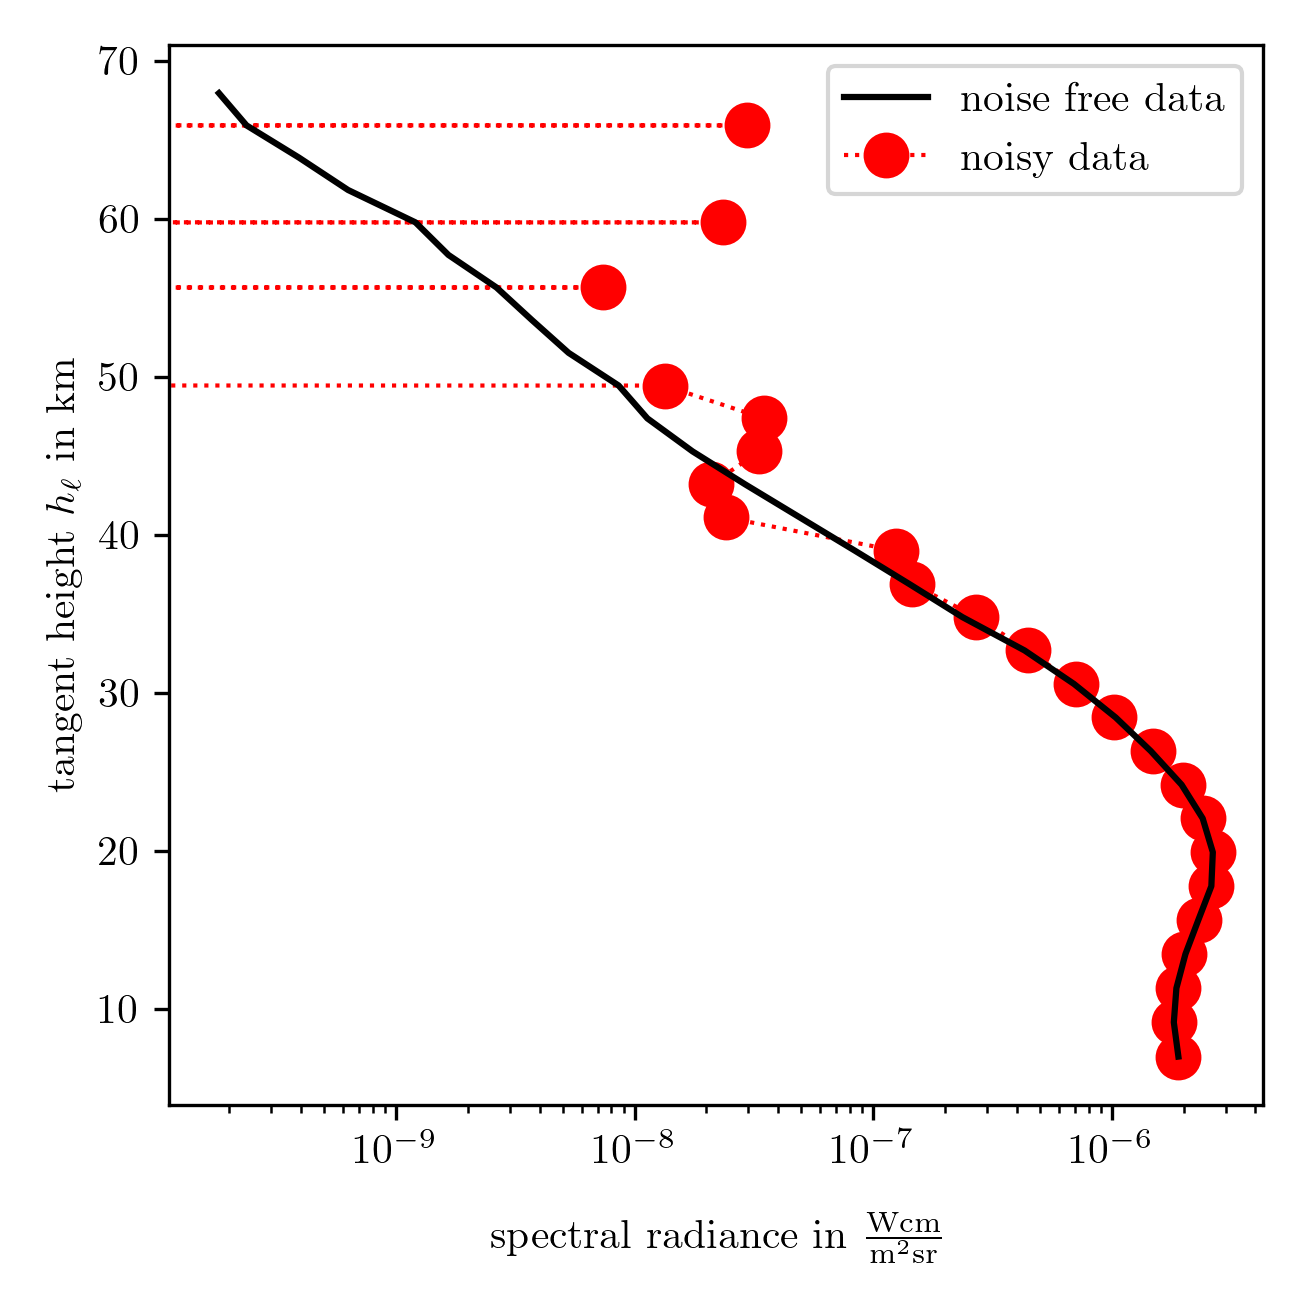
\includegraphics{DataPlot.png}
	\caption[Logarithmic plot of data points at different tangent height.]{Logarithmic plot of data points at different tangent height. Note that negative values are not appearing, and we see that the noise is dominating at high altitudes.}
	\label{fig:DataPlot}
\end{figure}
Now, given the data, we like to determine the posterior distributions over ozone $\bm{x}$, pressure $\bm{p}$ and temperature $\bm{T}$ at different heights.



\section{Hierarchical Bayesian Framework for Ozone}
\label{sec:BayModel}


\begin{figure}[htb!]
	\centering
	\begin{tikzpicture}
		\node[roundnode2] at (-4,6.5) (Q)     {$\bm{Q}$};
		\node[roundnode2] at (-2.5,5) (x)     {$\bm{x}$};
		\node[align=center] at (-1,4) (A)    {$\bm{A}_L$};
		\node[roundnode2] at (-1,2.5) (u)    {$\Omega$};
		\node[rectnode] at (-1,1) (y)    {$\bm{y}$};
		\node[roundnode2] at (-2.5,2.5) (e)    {$\bm{\eta}$};
		\node[roundnode2] at (-6.5,6.5) (S)    {$\bm{\Sigma}$};
		\node[roundnode2] at (-8,8) (s)    {$\gamma$};
		\node[roundnode2] at (-5.5,8) (d)    {$\delta$};
		
		%Lines
		\draw[->, very thick] (S) -- (e);
		\draw[->, mydotted, very thick] (s) -- (S);
		\draw[->, mydotted, very thick] (e) -- (y);
		\draw[->, very thick] (u.south) -- (y);
		\draw[->, mydotted, very thick] (A) -- (u);
		\draw[->, mydotted,  very thick] (x) -- (A.west);
		
		\draw[->, mydotted, very thick] (d) -- (Q); 
		
		\draw[->, very thick] (Q) -- (x); 
		%\node[align=center] at (0,4) (f3) {$= \bm{A}$};
		%\node[align=center] at (0.25,3.95) (f3) {$\approx \bm{M A}_L$};
		\node[align =center] at (-1,8) (T1) {marginal posterior \\ over hyper-parameters \\ $\pi(\gamma, \delta | \bm{y})$};
		\node[align =center] at (0,5) (T1) {conditional posterior \\ $\pi( \bm{x} |\gamma, \delta, \bm{y})$ };
		
		
		\node[fit=(s)(d),draw,dotted,black, rounded corners] {};
	\end{tikzpicture} 
	\caption[Directed acyclic graph for ozone retrieval and MTC scheme.]{Directed acyclic graph for modelling and measuring process of ozone highlighting the marginal and then conditional (MTC) scheme. The hyper-parameters $\delta$ and $\gamma$ determine the noise covariance $\bm{\Sigma} = \gamma^{-1}\bm{I}$ for the random noise vector $\bm{\eta} \sim \mathcal{N}(0, \gamma^{-1}\bm{I})$ and the prior precision matrix $\bm{Q} = \delta \bm{L}$ for the normal distribution over $\bm{x} \sim \mathcal{N}(0, \delta \bm{L})$, where $\bm{L}$ is a graph Laplacian, see Eq. \ref{eq:GLapl}. In the MTC scheme we evaluate the marginal posterior over the hyper-parameters $\pi(\gamma, \delta | \bm{y})$ as in Eq. \ref{eq:} first and then the conditional posterior $\pi(\bm{x}|\gamma,\delta,\bm{y})$ as in Eq. \ref{eq:CondPost}. The MTC scheme allows to evaluate the marginal posterior distribution over the hyper-parameters $\delta, \gamma$ independent of $\bm{x}$, breaking the correlation structure.
	Through the forward model $\bm{A}_{NL} \approx \bm{M}\bm{A}_L$ and the parameter $\bm{x}$ we generate a space of all measurable from which we randomly observe a data set $\bm{y}$ including random noise $\bm{\eta}$.}
	\label{fig:DAGO3}
\end{figure}

%Since the forward model described in Ch. \ref{ch:formodel} is weakly non-linear we will set up a linear Bayesian hierarchical framework first based on the linear forward model $\bm{A}_L$ and then later the approximated version $\bm{A}_{NL}\bm{M} \bm{A}_L$.
%Furthermore, the noise is normally distributed, so we establish a linear-Gaussian Bayesian hierarchical framework, aiming to recover an ozone profile and a pressure over temperature profile.
%In doing so, we first draw a directed acyclic graph (DAG) to visualise the measurement and modelling process and determine hyper-parameters and correlations between parameters.
%Then we define prior distributions over all parameters as well as a likelihood function so that we can formulate the posterior distribution.

In this section, we choose the prior distributions and describe the approach to evaluate the posterior distribution for ozone $\pi(\delta, \gamma, \bm{x}|\bm{y})$, conditioned on temperature and pressure, including the noise hyper-parameter $\gamma$.
Assuming Gaussian noise $\bm{\eta} \sim \mathcal{N}(0, \gamma^{-1} \bm{I})$, we define a linear-Gaussian Bayesian hierarchical model, see Sec. \ref{subsec:LinBay},
%\begin{subequations}
%	\begin{align}
%		\bm{y} |  \bm{x}, \gamma &\sim \mathcal{N}(\bm{A} \bm{x}, \gamma^{-1} \bm{I}) \label{eq:likelihood} \\
%		\bm{x} |  \delta &\sim \mathcal{N}(\bm{0}, (\delta \bm{L})^{-1}) \label{eq:xPrior} \\
%		\delta, \gamma &\sim \pi(\delta, \gamma) \label{eq:gammaPrior},
%	\end{align}
%	\label{eq:O3BayMode}
%\end{subequations}
with a normally distributed likelihood $\pi(\bm{y} |  \bm{x}, \gamma)$ including the forward model matrix $\bm{A}$ and prior distributions $\pi(\bm{x} |  \delta)$ and $\pi(\delta, \gamma)$, the noise covariance matrix $\gamma^{-1} \bm{I}$, the prior precision matrix $\delta \bm{L}$ and the prior mean set to zero, as in ~\cite{fox2016fast}.
The chosen Bayesian model is very similar to the regularisation approach, since we like to show that we receive much more meaningful results compared to a single regularisation solution.


\subsection{Prior Modelling}
To complete the Bayesian framework, we have to define prior distributions over the hyper-parameters and parameters.
Ideally, we define the prior distributions as uninformative as possible, and include functional dependencies and physical properties.
Here we can already see that our prior model is not taking into account that ozone values can not be negative, and we currently have no means to include that in a non-parametric approach.


First, we set the precision matrix of the prior distribution $\bm{x}|\delta$ to
\begin{align}
	\delta \bm{L} =
	\delta
	\begin{bmatrix}
		2 & -1 & & &  \\
		-1 & 2 & -1 & &   \\
		& \ddots & \ddots & \ddots &\\ 
		& & -1 & 2 & -1  \\
		& & & -1 & 2 
	\end{bmatrix} 
	\label{eq:GLapl} 
\end{align}
which is a 1-dimensional Graph Laplacian as in \cite{wang2015graphs,fox2016fast} with Dirichlet boundary condition.
This matrix will also act as the regulariser later in the Regularisation section, see Sec. \ref{sec:regularise}.
We reduce the dimension of $\bm{x}$ from $45$ to $34$ by discarding every second ozone VMR over a height of $\approx47$km.
Doing that, while not changing $\bm{L}$, we induce a larger correlation between points at higher altitude.
For $\delta$ and $\gamma$ we pick  relatively uninformative gamma distributions so that $\gamma \sim \mathcal{T}(\bm{\theta_{\gamma}}) \propto \gamma^{\alpha_\gamma -1 } \exp{( -\beta_\gamma \gamma) } $ and $\delta \sim \mathcal{T}(\bm{\theta_{\delta}})$, where $\bm{\theta_{\gamma}} = \{  \alpha_\gamma, \beta_\gamma\}  = \{ \alpha_\delta ,\beta_\delta\} = \bm{\theta_{\delta}} = (1,10^{-35})$, see Fig. \ref{fig:MargPostHistTT}, similar to \cite{fox2016fast}.
Here $ \alpha$ is the shape and $\beta$ is the rate parameter.
These gamma distributions have another advantage when using a MWG sampler to sample from the marginal posterior distribution $\pi(\gamma,\delta | \bm{y})$.
In doing so, we introduce the regularisation parameter $\lambda = \delta / \gamma $ so that $\pi(\gamma | \lambda, \bm{y}) \sim \mathcal{T}(\cdot)$ is gamma distribution and easy to sample from.
We plot the corresponding prior ozone profiles according to $\bm{x}\sim \mathcal{N}(0, (\delta \bm{L})^{-1})$ in Fig. \ref{fig:O3Prior}, where we see that the prior distribution is not informative but does include negative values.
See Tab. \ref{tab:priors} for a summary. 


\subsection{Posterior Distribution -- linear Model}
\label{sec:FirstO3Post}

\subsubsection{Marginal and Conditional Posterior}
\label{subsec:MTC}
As in Eq. \ref{eq:MTC}, we factorise the posterior
\begin{align}
	\pi( \bm{x}, \gamma, \delta| \bm{y}) \propto \pi(\bm{y}| \bm{x}, \gamma, \delta) \pi( \bm{x}, \gamma, \delta)
\end{align}
into 
\begin{align}
	\pi( \bm{x}, \gamma, \delta| \bm{y}) =\pi( \bm{x}|\gamma, \delta, \bm{y})\pi(\gamma, \delta | \bm{y})
\end{align}
the marginal posterior $\pi(\gamma, \delta | \bm{y})$ and conditional posterior $\pi( \bm{x}|\gamma, \delta, \bm{y})$.
Fox and Norton call this method the marginal and then conditional method (MTC) \cite{fox2016fast}, where we break the correlation structure between $\bm{x}$ and $\gamma, \delta$ as illustrated in Fig. \ref{fig:RueHeld} by marginalising over $\bm{x}$.
For the linear-Gaussian case, $\bm{x}$ cancels in the marginal posterior over the hyper-parameters, which we evaluate first and \textit{then} the conditional posterior of $\pi(\bm{x} | \gamma, \delta)$.

Consequently, for the hierarchical model specified in Eq.~\ref{eq:O3BayMode}, the marginal posterior distribution over the hyper-parameters is given by
\begin{align}
	\pi(\lambda, \gamma | \bm{y})
	\propto & \lambda^{n/2} \gamma^{m/2 }   \exp{ \Bigl\{ - \frac{1}{2} g ( \lambda) - \frac{\gamma}{2} f ( \lambda) \Bigr\} } \pi(\lambda, \gamma) \\
		\pi(\lambda, \gamma | \bm{y})
	\propto &  \lambda^{n/2} \gamma^{m/2 + 1}   \exp{ \Bigl\{ - \frac{1}{2} g ( \lambda) - \frac{\gamma}{2} f ( \lambda) - \beta_{\delta} \lambda  \gamma - \beta_{\gamma} \gamma \Bigr\}},
	\label{eq:MargPostAppl}
\end{align}
with the introduced regularisation parameter $\lambda = \delta / \gamma$, and
\begin{subequations}
	\label{eq:fandg}
	\begin{align}
		&f ( \lambda) = \bm{y}^T \bm{y} - (\bm{A}^T \bm{y})^T (\bm{A}^T  \bm{A} + \lambda \bm{L})^{-1} (\bm{A}^T \bm{y})  \label{eq:fAppl} \, ,  \\
		&\text{and } g(\lambda) = \log \det (\bm{A}^T  \bm{A} + \lambda \bm{L}) \label{eq:gAppl} \, ,
	\end{align}
\end{subequations}
see~\cite[Lemma 2]{fox2016fast}.
Note that, when changing variables from $\delta = \lambda \gamma$ to $\lambda$ the hyper-prior distribution changes to $\pi(\lambda) \propto \lambda^{\alpha_\delta-1} \gamma^{\alpha_\delta} \exp{(- \beta_\delta \lambda  \gamma)} $, due to $\text{d}\delta / \text{d} \lambda = \gamma$.
\begin{figure}[ht!]
	\centering
	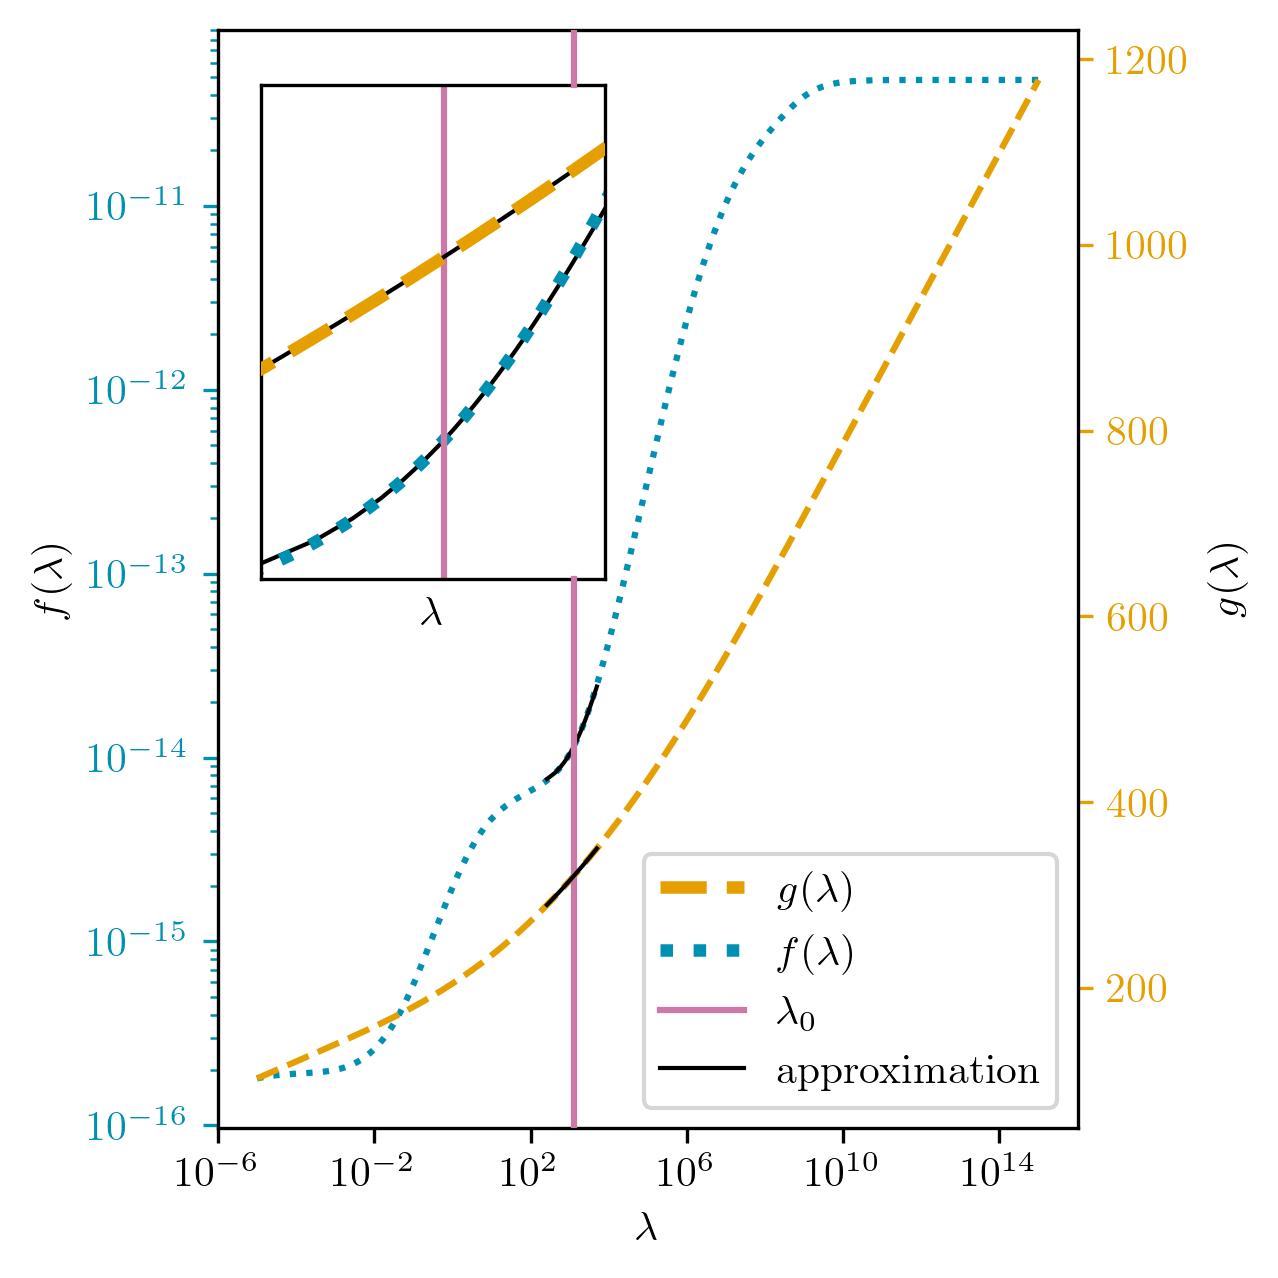
\includegraphics{f_and_g_phd.png}
	\caption[Plot of the functions $f(\lambda)$ and $g(\lambda)$ for marginal posterior.]{Plot of the functions $f(\lambda)$ and $g(\lambda)$ from the marginal posterior for a wide range of $\lambda = \delta / \gamma$. We plot the third-order Taylor series in black around the mode of the marginal posterior (vertical line) for the sampling range of $\lambda$ within the MWG algorithm.}
	\label{fig:fandg}
\end{figure}
Most of the computational effort, for each function evaluation of the marginal posterior in Eq. \ref{eq:MargPostAppl}, lies in the calculation of $f(\lambda)$ in Eq. \ref{eq:fAppl} and $g(\lambda)$ in Eq. \ref{eq:gAppl}.
In  Fig. \ref{fig:fandg} we see that $f(\lambda)$ and $g(\lambda)$ are well behaved within the region of interest and approximate $f(\lambda) \approx \tilde{f}(\lambda)$ with a 3rd order Taylor series around the mode $\lambda_0$ of $\pi(\lambda, \gamma | \bm{y})$.
We also note that $\tilde{g}(\lambda) \approx g(\lambda)$ behaves linearly around $\lambda_0$ in the log-space.
The approximations are implicitly given by
\begin{align}
	f^{(r)}& (\lambda_0)= (-1)^{r+1} (\bm{A}^T \bm{y})^T (\bm{B}_0^{-1} \bm{L})^r \bm{B}_0^{-1} \bm{A}_L^T \bm{y} \label{eq:ftay}  \\
	\text{and } & \log{ \tilde{g}(\lambda)} = (\log{\lambda} - \log{\lambda_{0}})  \frac{ \log{g(\lambda_{\text{max}})} - \log{g(\lambda_{0})} }{\log{\lambda_{\text{max}}} - \log{\lambda_{0}} } + \log{ g(\lambda_{0})} 
	\label{eq:gtay}
\end{align} 
with $\bm{B}_0 = \bm{A}^T  \bm{A} + \lambda_0 \bm{L}$.
We plot the approximations
\begin{subequations}
	\label{eq:fandg}
	\begin{align}
		&\tilde{f} ( \lambda) = \sum^3_{r=0} 	f^{(r)}(\lambda_0) (\lambda-\lambda_0)^r  \label{eq:fAprox} \, ,  \\
		&\text{and } \tilde{g} (\lambda) = \exp \log{\tilde{g}(\lambda)}  \label{eq:gAprox} \, ,
	\end{align}
\end{subequations} in Fig. \ref{fig:fandg} and elaborate on the approximation errors in Sec \ref{sec:fgErros}.
Note that usually a Taylor series includes a factor $(r!)^{-1}$, in this case it cancels in $f^{(r)}(\lambda_0)$, see \cite{fox2016fast}.

Using these approximation we can either utilise a TT approximation of the marginal posterior, see Sec. \ref{subsec:TTMarg}, over a predefined grid and calculate the marginals $\pi(\gamma|\bm{y})$ and $\pi(\lambda|\bm{y})$, or employ a Metropolis within Gibbs (MWG) sampler to sample from $\pi(\gamma,\lambda|\bm{y})$, see sec. \ref{subsec:MWG}.
More specifically, we implement a Metropolis random walk on
\begin{align}
	\label{eq:margApplCondGam}
	\pi(\lambda | \gamma, \bm{y}) &\propto \lambda^{n/2+\alpha_\delta -1} \exp{\Bigl\{ - \frac{1}{2} g ( \lambda) - \frac{\gamma}{2} f ( \lambda) - \beta_\delta \gamma \lambda \Bigr\}}.
\end{align} 
We accept or reject a proposal $\lambda^{\prime} \sim \mathcal{N}(0, \sigma_{\lambda})$ according to the acceptance ratio in log space
\begin{align} 
	\log \left\{ \frac{\pi(\lambda^{\prime} | \gamma^{(k)}, \bm{y})  }{\pi(\lambda^{(k)}| \gamma^{(k)}, \bm{y})}  \right\} 
	= \log  \{\pi(\lambda^{\prime} | \gamma^{(k)}, \bm{y} ) \}  -\log  \{ \pi(\lambda^{(k)}| \gamma^{(k)}, \bm{y}) \} \\
	= \frac{n}{2} (\log\{\lambda^{\prime}\} - \log\{\lambda^{(k)}\} ) + \frac{1}{2} \Delta g + \frac{\gamma^{(k)}}{2} \Delta f  + \beta_\delta \gamma^{(k)} \Delta \lambda  \, ,
\end{align}
where $\Delta \lambda = \lambda^{\prime} - \lambda^{(k)} $ and  $\Delta f \approx \tilde{f}(\lambda^\prime) - \tilde{f}(\lambda^{(k)}) = \sum^3_{r = 1} f^{(r)} (\lambda_0) (\Delta \lambda^\prime - \Delta \lambda^{(k)})^r $, with  $\Delta \lambda^{\prime} = \lambda^\prime - \lambda_0 $ and $\Delta \lambda^{(k)} =  \lambda^{(k)} - \lambda_0$.
Similarly we approximate $\Delta g \approx \tilde{g}(\lambda^{\prime}) -\tilde{g}(\lambda^{(k)})$.
Lastly, we do a Gibbs step on
\begin{align}
	\gamma^{(k+1)} |  \lambda^{(k+1)}, \bm{y} &\sim \Gamma \bigg( \frac{m}{2} + \alpha_\delta + \alpha_\gamma, \frac{1}{2} f (\lambda^{(k+1)}) + \beta_\gamma + \beta_\delta \lambda^{(k+1)} \bigg)\label{eq:GibbsStep}
\end{align} 
to generate marginal posterior samples $(\lambda, \gamma)^{(1)}, \dots, (\lambda, \gamma)^{(N)} \sim  \pi(\lambda, \gamma| \bm{y})$.

Then we evaluate the normally distributed conditional posterior distribution
\begin{align}
	\bm{x}| \delta, \gamma, \bm{y}  \sim \mathcal{N}\big( \underbrace{ (\bm{A}^T \bm{A} + \delta / \gamma \bm{L} )^{-1} \bm{A}^T \bm{y}}_{\bm{x}_{\lambda}}, ( \underbrace{ \gamma \bm{A}^T \bm{A} + \delta \bm{L} }_{\gamma \bm{B}_{\lambda}}  )^{-1} \big) \, \label{eq:CondPost},
\end{align}
as in Eq. \ref{eq:CondPostLin}.
In this thesis, we compute the mean
\begin{align}
	\mu_{\bm{x}|\bm{y}} = \int \bm{x}_{\lambda} \pi(\lambda| \bm{y}) \text{d}\lambda \approx \sum \bm{x}_{\lambda_i} \pi(\lambda_i| \bm{y}) \, , \label{eq:MeanInt}
\end{align} and covariance
\begin{align}
	\Sigma_{\bm{x}|\bm{y}} = \int \gamma^{-1}  \pi(\gamma | \bm{y} ) \, \text{d} \gamma \, \int  \bm{B}_{\lambda}^{-1} \, \pi(\lambda | \bm{y} )  \, \text{d} \lambda  \approx \sum {\gamma_i}^{-1}\pi(\gamma_i| \bm{y}) \sum \bm{B}_{\lambda_i}^{-1}\pi(\lambda_i| \bm{y})\, \label{eq:CovInt}
\end{align}
of $\pi(\bm{x}| \delta, \gamma, \bm{y})$ as weighted expectations, by quadrature \cite[Sec. 2.1]{Dick_Kuo_Sloan_2013}, with $\sum \pi(\lambda_i| \bm{y}) = \sum \pi(\gamma_i| \bm{y}) = 1$.
The weights $\pi(\lambda_i| \bm{y})$ and $\pi(\gamma_i| \bm{y})$ are either given by the TT approximation or by the bins for the sample-based histograms.
If calculating the variance is too costly, the randomise then optimise method as in \cite{bardsley2015randomize, fox2016fast} may be a feasible alternative to draw a sample from Eq. \ref{eq:CondPost}.



%
%We find the mode at the minimum of  $-\log\{ \pi(\lambda, \gamma | \bm{y}) \}$  using \texttt{scipy.optimize.fmin} function and limit the number of function evaluation to 25 and use Cholesky back and forward substitution to calculate values of $g(\lambda)$ and $f(\lambda)$.
%Additionally, we calculate $\bm{B}_0^{-1} \bm{L} $ and  $\bm{B}_0^{-1}  \bm{A}_L^T \bm{y}$ once more at $\lambda_0$ and plot the Taylor approximation within the sampling region in Fig. \ref{fig:fandg}.



%\subsection{Posterior distributions with Linear model for Ozone -- MTC}
%\label{sec:firstMTC}
%In this section we calculate the posterior marginal and then conditional (MTC) posterior distribution for ozone conditioned on the ground truth temperature and pressure profiles using the linear forward model $\bm{A}_L$.
%This is faster then the other way round (finding temperature over pressure conditioning on ozone) and temperature and pressure are well defined within the atmosphere so it is easier to just condition on a temperature and pressure profile out of a text book.
%We employ a so-called Metropolis within Gibbs (MWG) algorithm on the marginal posterior as summarised in the algorithmic Box \ref{alg:margPost} or use a Tensor-Train (TT) approximation to calculate marginal posterior values.
%Then we can either sample from the conditional posterior using the randomise then optimise (RTO) method or calculate conditional mean and variance using quadrature.


%The DAG in Fig. \ref{fig:DAGO3} visualises that process and we can show explicitly that we group the hyper-parameters $\delta, \gamma$ together to determine the marginal posterior $\pi(\gamma, \delta | \bm{y})$.
%Here $\gamma$ , the noise parameter, determines the noise precision $\bm{\Sigma} = \gamma ^{-1} \bm{I}$ and $\delta$, the smoothness parameter, the precision matrix $\bm{Q} = \delta \bm{L}$ of the prior distribution for $\bm{x}$.
%Then conditioned on the hyper-parameters the conditional posterior $\pi( \bm{x} |\gamma, \delta, \bm{y})$ gives the distribution of posterior ozone profiles.
%Note that we use the linear model $A_L$ here as we do not have an approximation to the non-linear model yet and all prior distributions are defined in Table \ref{tab:priors}.
%The full posterior $\pi(\bm{x},\gamma, \delta | \bm{y}) =  \pi(\bm{x}|\gamma, \delta ,\bm{y}) \pi(\gamma, \delta | \bm{y}) $ is given by multiplication of the marginal and conditional posterior densities. 

%\begin{align}
%	\bm{x} |  \bm{\theta}, \bm{y} \sim \mathcal{N} \Big(
%	\underbrace{\bm{\mu} + \left( \bm{A}^T \bm{\Sigma}^{-1} \bm{A} + \bm{Q} \right)^{-1} \bm{A}^T \bm{\Sigma}^{-1} (\bm{y} - \bm{A} \bm{\mu})}_{\bm{\mu}_{\bm{x} |  \bm{\theta}, \bm{y}}},
%	\underbrace{ \left( \bm{A}^T \bm{\Sigma}^{-1} \bm{A} + \bm{Q} \right)^{-1} }_{\bm{\Sigma}_{\bm{x} |  \bm{y}, \bm{\theta}}}
%	\Big) \, ,
%\end{align}
%is normal distribution and we compute weighted expectations, as in Eq.~\ref{eq:MargExpPos}, of the conditional mean and covariance matrix, where the weights are given by $\pi(\bm{\theta} | \bm{y})$. 
%Note that both the noise covariance $\bm{\Sigma} = \bm{\Sigma}(\bm{\theta})$ and the prior precision matrix $\bm{Q} = \bm{Q}(\bm{\theta})$ depend on the hyper-parameters $\bm{\theta}$.


Within the MTC scheme we determine the marginal posterior distribution $\pi(\gamma, \lambda| \bm{y})$ over the hyperparameters $\delta$  and $\lambda = \delta / \gamma$ first and then the mean and covariance of the full posterior distribution $\pi(\bm{x}|\bm{y})$ as in Eq. \ref{eq:MeanInt} and \ref{eq:CovInt}.
We set $\bm{A} \coloneqq  \bm{A}_L$ and approximate $f(\lambda)$  and $g(\lambda)$ around the mode $( \lambda_{0}, \gamma_0 )$ of the marginal posterior distribution, see Eq. \ref{eq:MargPostAppl}.
The mode is provided by the \texttt{scipy.optimize.fmin} function.
In doing so, we compute the vector $\bm{B}_0^{-1}\bm{A}^T\bm{y} = (\bm{A}^T\bm{A} + \lambda_0 \bm{L})\bm{A}^T\bm{y} $, the matrix $\bm{B}_0^{-1}\bm{L}$ and the determinant in $g(\lambda)$ using Cholesky decomposition.
Then we approximate $f(\lambda)$ with a 3rd order Taylor series and $g(\lambda)$ with a linear approximation in the log-space, where for the approximation in $g(\lambda)$ we set $\lambda_{\text{max}}$ to the maximum value of $\lambda$ on the TT-grid, see Tab. \ref{tab:priors}.
\begin{figure}[ht!]
	\centering
	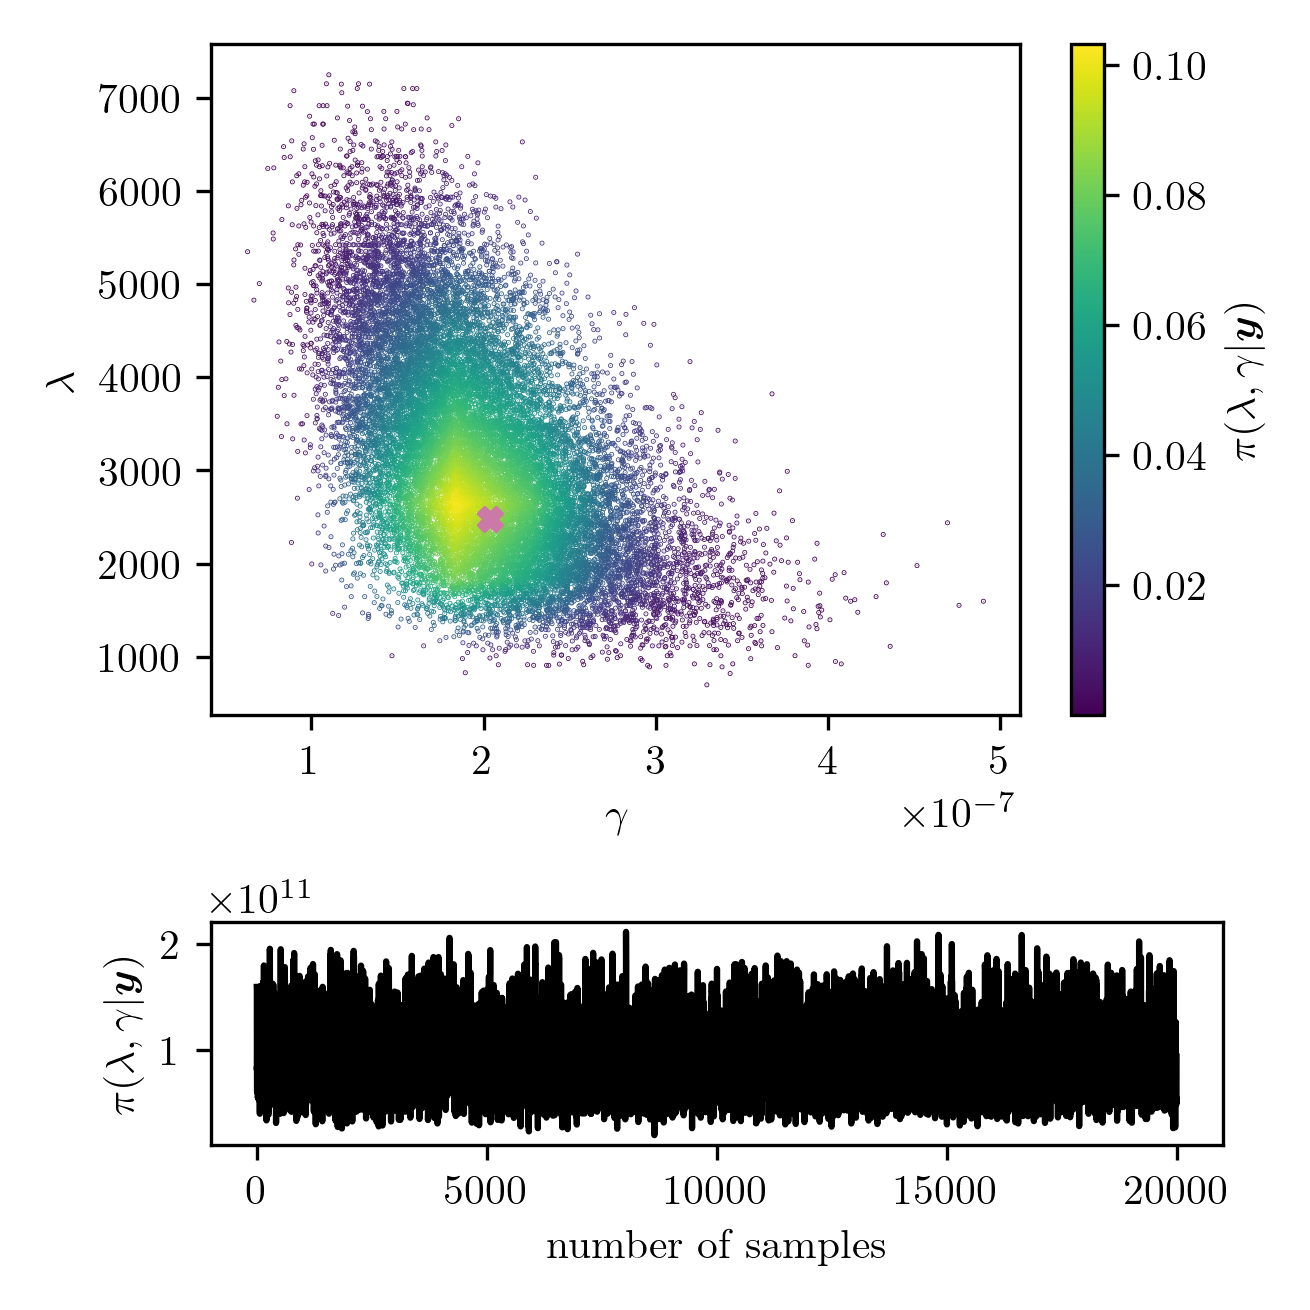
\includegraphics{ScatterplusHistoPlusTT.png}
	\caption[Scatter plot of samples from marginal posterior, including weighting from TT approximation; trace plot of the marginal posterior samples.]{We scatter plot the samples of $\lambda = \delta / \gamma $ and $\gamma$ from the marginal posterior $\pi(\lambda , \gamma  | \bm{y})$ and colour code the samples using the TT approximation of $\pi(\lambda , \gamma  | \bm{y})$. The mode of $(\lambda_0 , \gamma_0)$ of $\pi(\lambda , \gamma  | \bm{y})$ is marked by the pink cross. To show ergodicity we plot the trace of the samples of the MWG sampler below.}
	\label{fig:ScatterPlotTT}
\end{figure}


\subsubsection{Tensor-train Approximation of the Marginal Posterior Distribution}
\label{subsec:firstMargTT}
We approximate the square root of marginal posterior on a predefined univariate grid, where $\gamma = [ 0.1 \times 10^{15}, 6 \times 10^{15}]$ and $\lambda = [ 100, 5000]$.
We set the number of grid points to $n = 20$ and the number of ranks $r = 5$, which we keep constant.
Since we do not approximate $\sqrt{ \pi(\gamma, \lambda| \bm{y}) }$ in the log-space we introduce a "normalisation constant" $c = 340$. This avoids underflow so that the values $\sqrt{\pi(\gamma, \lambda| \bm{y})} = \exp \{ 0.5 \log  \pi(\gamma, \lambda| \bm{y}) + c \} $ are within computer precision.
Then we initialise the \texttt{tt.cross.rectcross.rect\_cross.cross} function, based on the rect cross algorithm in \cite{OSELEDETS2010TTCross}, from the Python package \texttt{ttpy} \cite{Oseledets2018ttpy}, with a random tensor and do 3 sweeps to obtain an TT approximation of $\pi(\gamma, \lambda| \bm{y})$.
This takes about $0.1s$ for $600$ function evaluations.
Then we compute the marginals $\pi(\lambda| \bm{y})$ and $\pi(\gamma| \bm{y})$ as described in Sec. \ref{subsec:TTMarg}.
In doing so we calculate the coefficient tensor $\bm{B}$ and $\bm{B}_{\text{pre}}$ as in Prop. \ref{prob:backMarg} and \ref{prob:ForMarg}, where we set $\xi = 1 / \uplambda (\mathcal{X})$ and $\uplambda(x) = 1$, so that for Cartesian basis $\bm{M}_k = \text{diag}(\uplambda_k(\mathcal{X}_k))$ in Eq. \ref{eq:MassMat}.
We plot the TT approximation as a colour map on top of the obtained samples in the scatter plot in Fig. \ref{fig:ScatterPlotTT}.

\subsubsection{Sample from Marginal Posterior Distribution}
\label{subsec:firstMarg}
To sample from $\pi(\gamma, \lambda| \bm{y})$ we employ the MWG algorithm , see Alg. Box \ref{alg:MwG} and Sec. \ref{subsec:MTC}.
We initialise the MWG at the mode $(\lambda^{(0)} , \gamma^{(0)}  ) = ( \lambda_{0} , \gamma_{0}  )$ and take $N = 10000$ plus $N_{\text{burn-in}} = 100$ steps in approximately $0.3$s.
The standard deviation of the normal proposal distribution is set to $\sigma_{\lambda} = 0.8 \lambda_0$ so that the acceptance rate is $\approx 0.5$ as suggested in \cite{robertsLecNot}.
The samples are plotted in Fig. \ref{fig:ScatterPlotTT} as a 2D scatter plot, as well as the trace of the MWG to show ergodicity.
We calculate the integrated autocorrelation time (IACT) with the Python implementation of \cite{wolff2004monte}, provided by \cite{drikHesse}, which gives us $\tau_{\text{int}, \gamma} = $ and $\tau_{\text{int}, \delta} = $, see Fig. \ref{fig:IATCLamLin} and Fig. \ref{fig:IATCGamLin}.
\begin{figure}[ht!]
	\centering
	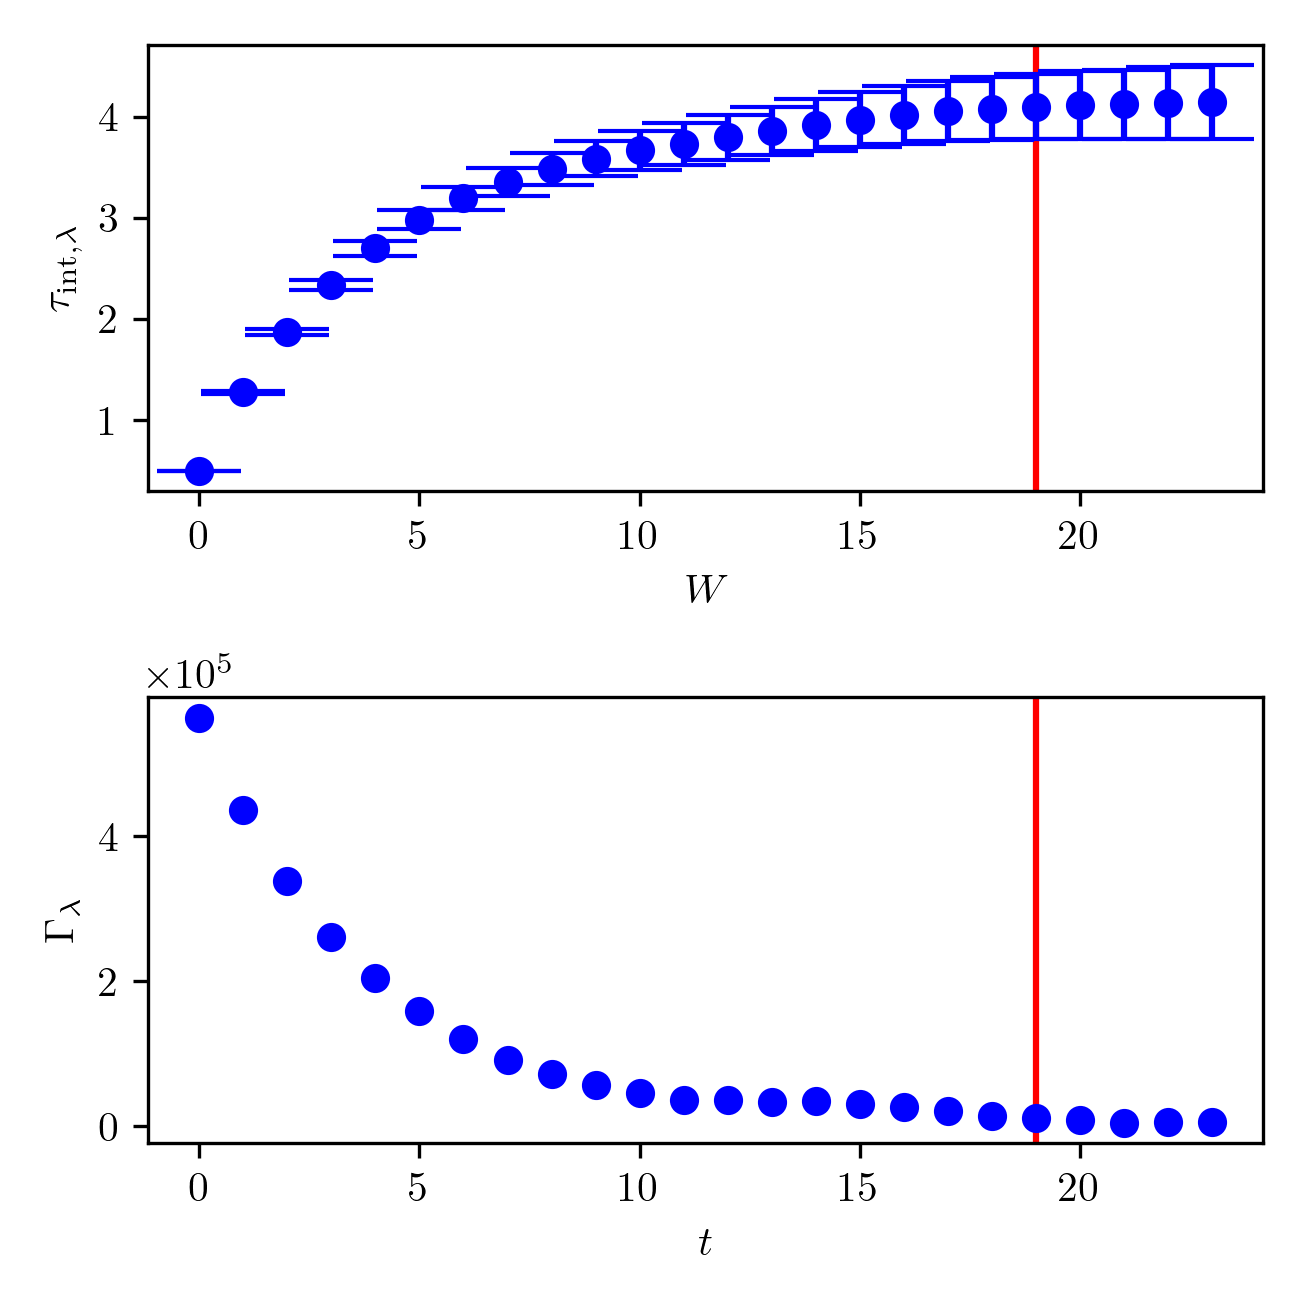
\includegraphics{UwerrTauIntFirstO3lam.png}
	\caption[IATC of $\lambda$ samples from $\pi(\gamma, \lambda| \bm{y})$, for linear model.]{Here the autocorrelation function $\Gamma_{\lambda}$ at different lags W is plotted as well as the IATC $\tau_{\text{int},\lambda}$ for the samples from $\pi(\gamma, \lambda| \bm{y})$ based on the linear forward model.}
	\label{fig:IATCLamLin}
\end{figure}
\begin{figure}[ht!]
	\centering
	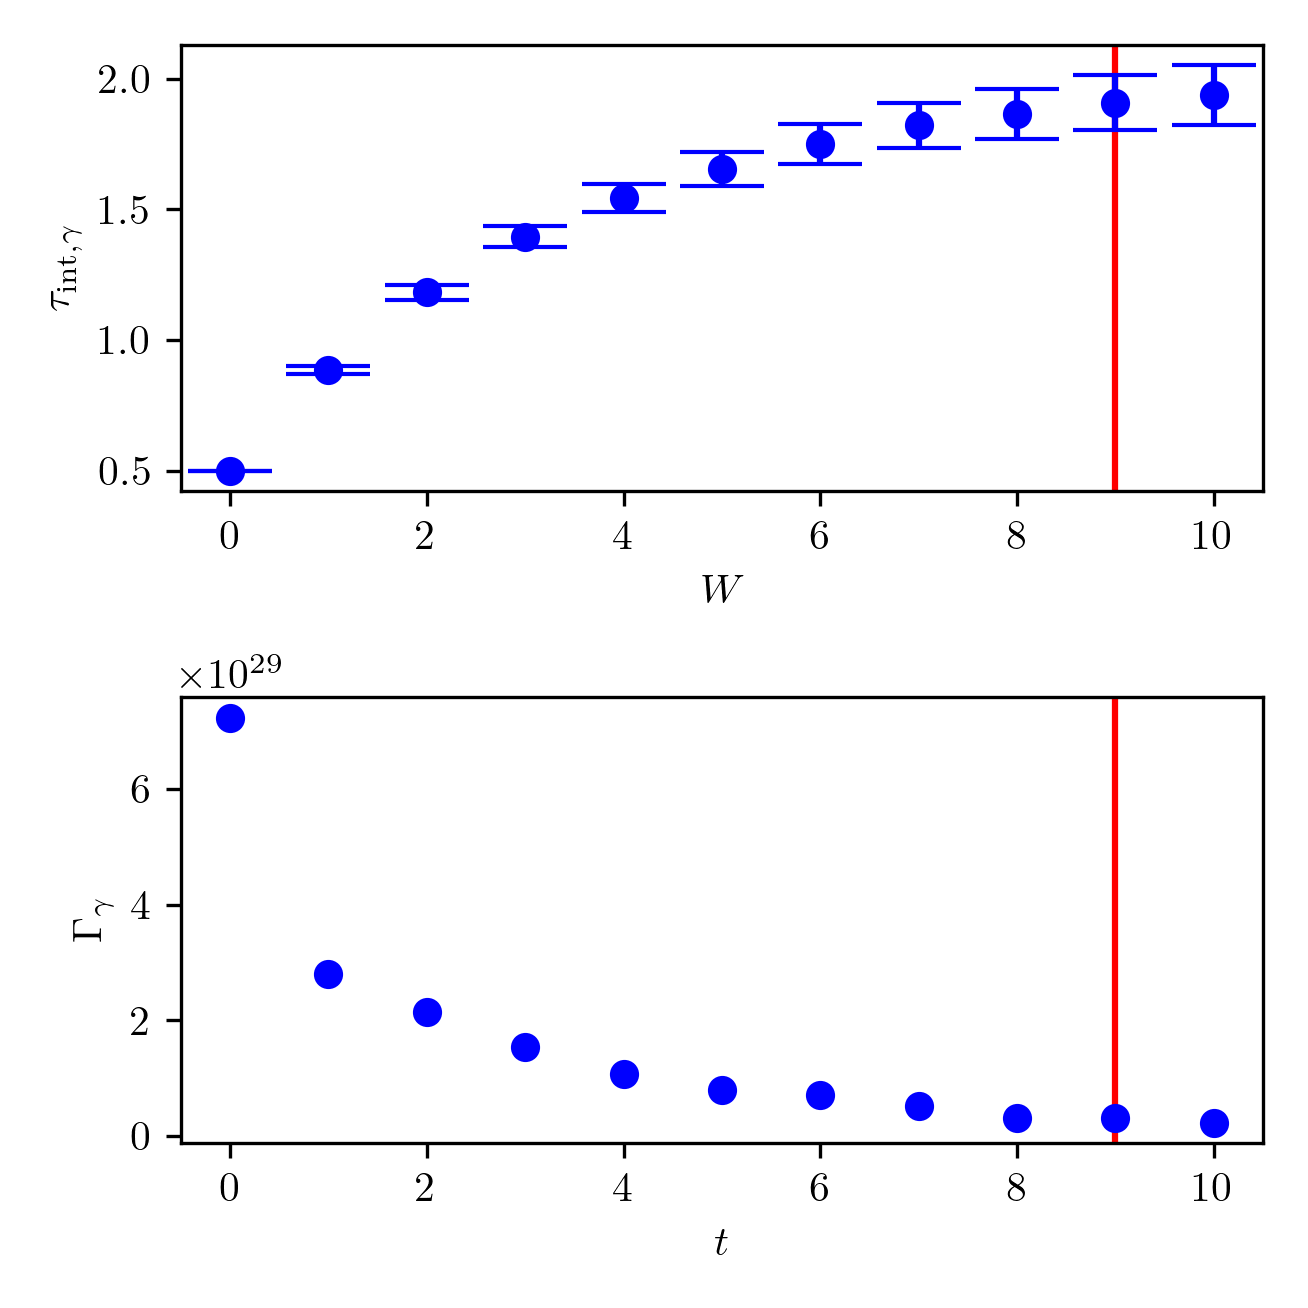
\includegraphics{UwerrTauIntFirstO3gam.png}
	\caption[IATC of $\gamma$ samples from $\pi(\gamma, \lambda| \bm{y})$, for linear model.]{Here the autocorrelation function $\Gamma_{\gamma}$ at different lags W is plotted as well as the IATC $\tau_{\text{int},\gamma}$ for the samples from $\pi(\gamma, \lambda| \bm{y})$ based on the linear forward model.}
	\label{fig:IATCGamLin}
\end{figure}
\clearpage
%\begin{algorithm}[!ht]
%	\caption{Metropolis within Gibbs for $\pi(\lambda, \gamma | \bm{y})$}
%	\begin{algorithmic}[1]
%		\STATE Initialise  \( \bm{\theta}^{(0)}  =( \lambda^{(0)} , \gamma^{(0)}  ) \) and set burn-in $N_{\text{burn-in}}$
%		\FOR{ \( k = 1, \dots, N^{\prime} \)}
%		\STATE Propose \( \lambda \sim \mathcal{N}(\lambda^{(t-1)}, 0.8 \lambda_0)  \)
%		\STATE Compute
%		\[ \alpha( \lambda  | \lambda^{(t-1)}) = \min \left\{ 1, \frac{\pi(\lambda | \gamma^{(t-1)}, \bm{y})  }{\pi(\lambda^{(t-1)}| \gamma^{(t-1)}, \bm{y})}  \right\} \]
%		\STATE Draw $u \sim \mathcal{U}(0,1)$
%		\IF{$\alpha \geq u$ }
%		\STATE Accept and set \( \lambda^{(t)} = \lambda \)
%		\ELSE  
%		\STATE Reject and keep \(\lambda^{(t)} = \lambda^{(t-1)} \)
%		\ENDIF
%		\STATE Draw $\gamma^{(t)} | \lambda^{(t)} ,\bm{y} \sim \text{Gamma} \big( 0.5  \, m + 2, 0.5 \, f(\lambda^{(t)}) + 10^{-10}(1 + \lambda^{(t)}) \big) $
%		\ENDFOR
%		%\STATE Output: $ \bm{\theta}^{(N_{\text{burn-in}})}, \dots,  \bm{\theta}^{(k)} , \dots,   \bm{\theta}^{(N)} \sim \pi(\bm{\theta}| \bm{y}) $
%		\STATE Output: $ (\lambda, \gamma)^{(N_{\text{burn-in}})}, \dots,  (\lambda, \gamma)^{(k)} , \dots,   (\lambda, \gamma)^{(N)} \sim \pi(\lambda, \gamma| \bm{y}) $
%	\end{algorithmic}
%	\label{alg:margPost}
%\end{algorithm}

\subsubsection{Full Conditional Posterior of Ozone}
\label{subsec:firstCond}
Based on the marginal posterior distribution $\pi(\gamma, \lambda | \bm{y})$ we calculate the mean and covariance of the conditional posterior $\pi(\bm{x} | \gamma, \lambda, \bm{y})$ by quadrature as in Eq. \ref{eq:MeanInt} and Eq. \ref{eq:CovInt}.
We can either use the sample based histogram bins as weights or the TT-approximation to integrate over marginals of $\pi(\gamma, \lambda | \bm{y})$.

By binning the output samples from the MWG, see Fig. \ref{fig:ScatterPlotTT}, into a normalised histogram with 20 bins, we obtain empirical "function values" of the marginal posterior.
With the height of the histogram bars as quadrature weights, e.g. $\pi(\lambda_i| \bm{y})$ at the centre $\lambda_i$ of each bin, we calculate the full conditional mean $\bm{\mu}_{\bm{x}|\bm{y}}$ and covariance matrix $\bm{\Sigma}_{\bm{x}|\bm{y}}$ as weighted expectations.
Similarly, we use the approximations of $\pi(\lambda| \bm{y})$ and $\pi( \gamma | \bm{y})$ to perform this calculation.
Again, we use Cholesky decomposition to invert $\bm{B}_{\lambda} = \bm{A}^T \bm{A} + \lambda \bm{L}$ and to calculate $\bm{x}_{\lambda} = (\bm{A}^T \bm{A} + \lambda \bm{L} )^{-1} \bm{A}^T \bm{y}$.
In total that we have to evaluate $\bm{x}_{\lambda}$ and invert $\bm{B}_{\lambda}$ 20 times to obtain mean and covariance of $\pi(\bm{x}|\bm{y})$, Fig. \ref{fig:O3Samp}, which takes less than $0.2$s.
We plot posterior samples of $\pi(\bm{x}|\bm{y})$ in Fig. \ref{fig:O3Samp}, where we set negative values ozone VMR to zero.
The sample mean is slight larger than posterior mean at heights where the data is noise dominated, and the ozone values are determined by the prior, or where the ground truth is close to zero.
This indicates that we should use a different more physical based prior especially at higher altitudes, e.g. parametrise the ozone profile.
Note, that the posterior samples do not represent the ozone peak at around $80$km.
\begin{figure}[ht!]
	\centering
	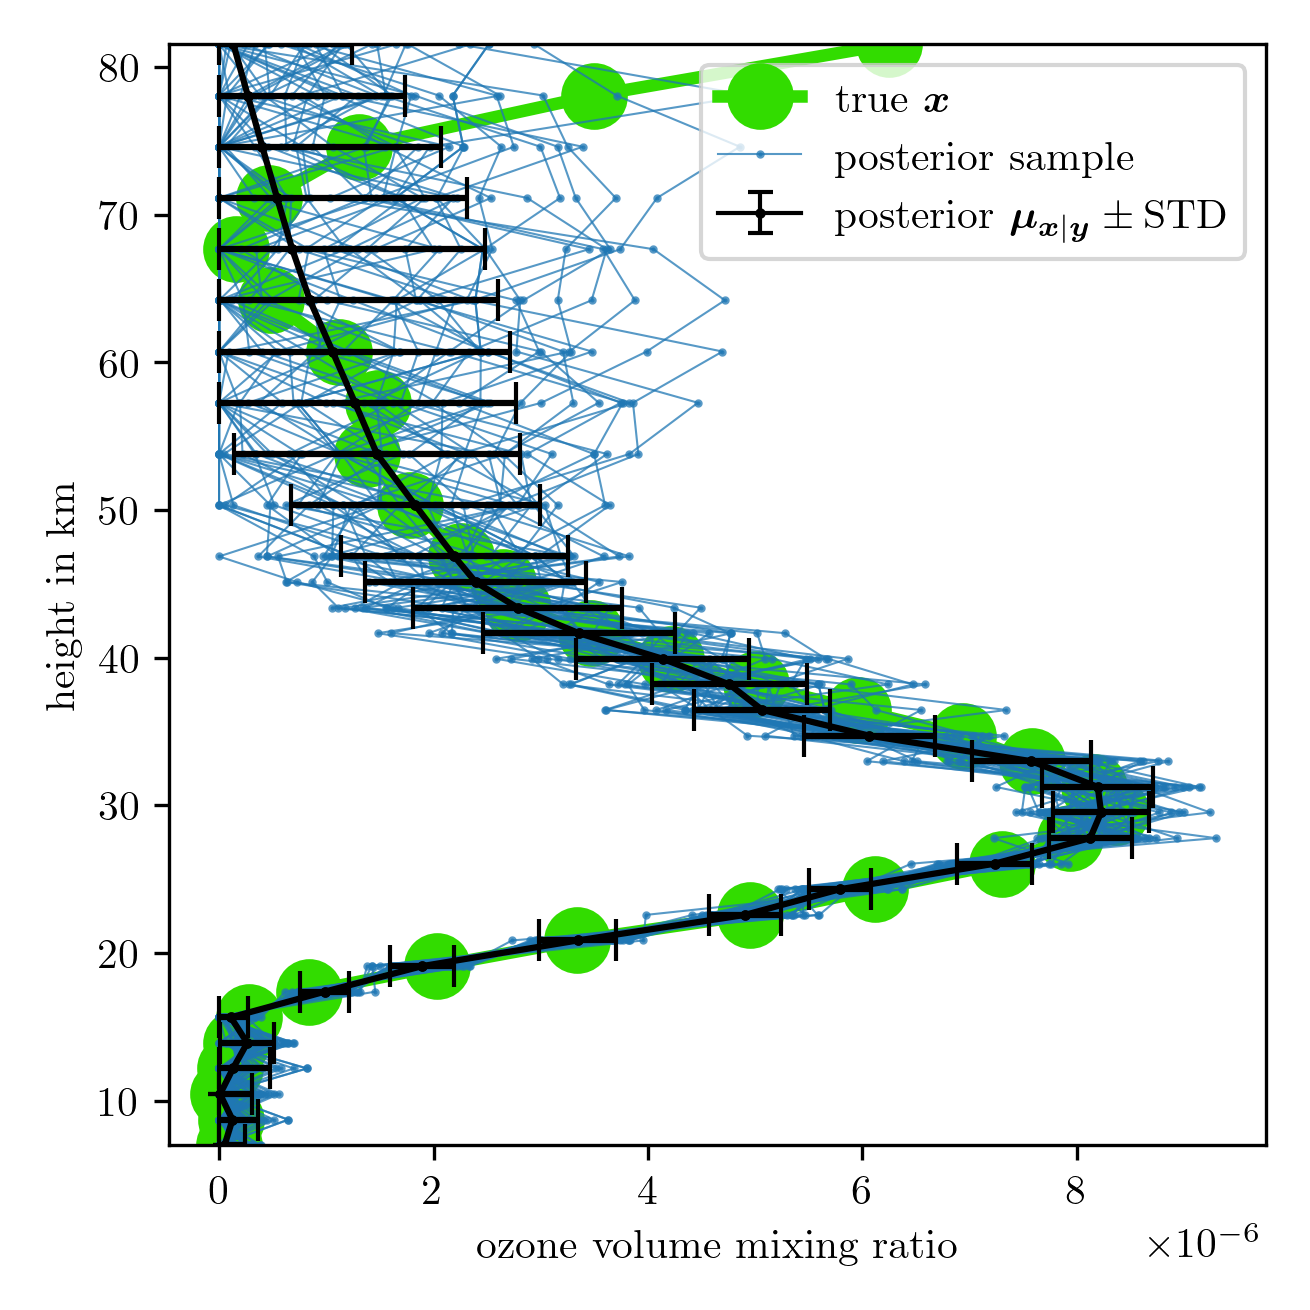
\includegraphics{FirstTestRes.png}
	\caption[Ozone samples of the full posterior.]{We draw ozone samples from the full posterior distribution $\pi(\bm{x}| \bm{y})$ after characterising mean and covariance of $\pi(\bm{x}| \bm{y})$ by weighted expectations over the marginal posterior $\pi(\lambda,\gamma | \bm{y})$. we determine  $\pi(\lambda,\gamma | \bm{y})$ either through sampling or via TT approximation based on the linear forward map $\bm{A}_L$. Note that we set negative values ozone VMR values to zero. We will use those samples to find the affine map $\bm{M}$, see section \ref{sec:affineMap}}
	\label{fig:O3Samp}
\end{figure}
\clearpage
%\subsubsection{Randomize then optimize -- RTO}
%For the RTO method we start by drawing an independent hyper-parameter sample $ ( \delta, \gamma) \sim \pi(\delta, \gamma | \bm{y})$ from the samples of the MwG.
%Then we generate two independent Gaussian random variables $\bm{v}_1 \sim \mathcal{N}(\bm{0},\gamma  \bm{A}^T_L \bm{A}_L)$ and $\bm{v}_2 \sim \mathcal{N}(\bm{0}, \delta \bm{L})$.
%Here  can use Cholesky factorisation of $\bm{L} =\bm{L}_C\bm{L}^T_C $ and the multiplication rule for normal distributions so that $\bm{v}_1 \sim \sqrt{\gamma} \bm{A}_L^T \mathcal{N}(0,\bm{I})$ and $\bm{v}_2 \sim \sqrt{\delta} \bm{L}_C \mathcal{N}(0,\bm{I})$.
%Then we solve
%\begin{align}
%	\label{eq:FirstRTO}
%	\left( \gamma \bm{A}_L^T  \bm{A}_L +\delta \bm{L} \right) \bm{x} = \gamma \bm{A}_L^T \bm{y} + \bm{v}_1 + \bm{v}_2 \, ,
%\end{align}
%using Cholesky back and forward substitution, for $\bm{x}$ and obtain one independent sample of $\pi(\bm{x}|\bm{y}, \bm{\theta})$.
%See Fig. \ref{fig:O3Samp}, where we plot $m = $ samples of the conditional posterior.
%
%The histogram in is binned as we intergate over it to 7 bins

\section{Approximate non-linear Forward Model with an Affine Map} 
\label{sec:affineMap}
Given the posterior distribution for ozone $ \pi(\bm{x}|\bm{y})$, we can now approximate the non-linear forward model 
\begin{align}
	\bm{A}_{NL} \approx \bm{M A}_L = \bm{A} \, ,
\end{align}
with an affine map $\bm{M}$, see Fig. \ref{fig:affinStrat} for the summarised strategy.
We focus on the posterior distribution of ozone profiles conditioned on pressure and temperature.
Since this as is a much quicker process, when using the MTC method, compared to obtaining the pressure and temperature posterior distributions.
\begin{figure}[htb!]
	\centering
	\begin{tikzpicture}
		\node[rectnode] at (0,0) (Oy)    {$\bm{y}$};
		\node[roundnode2] at (0,-2) (x)     {$\bm{x}$};
		\node[rectnode] at (-1.75,-4) (NLy)    {$\bm{V}$};%{$\bm{A}_{NL}\bm{x}$};
		\node[rectnode] at (1.75,-4) (y)    {$\bm{W}$};%{$\bm{A}_L\bm{x}$};
		\draw[->, very thick] (Oy.south) -- (x.north); 
		\draw[->, very thick] (x.south west) -- (NLy.north); 
		\draw[->, very thick] (x.south east) -- (y.north); 
		\draw[->, very thick] (NLy.east) -- (y.west); 
		\node[align=center] at (1,0) (l1) {Data};
		\node[align=center] at (3.5,-2) (f2) {Ozone Profiles from $\pi(\bm{x}|\bm{y}) $};
		\node[align=center] at (1.75,-1) (l1) {$\pi(\lambda , \gamma  | \bm{y})$ with $\bm{A}_L$};
		
		\node[align=center] at (-4.75,-4) (f3) {non-linear forward model};
		\node[align=center] at (4.25,-4) (f4) {linear forward model};
		\node[align=center] at (0,-5) (f5) {$\bm{A}_{NL} \approx \bm{M A}_L= \bm{A}$ };
		
		\node[align=center] at (0,-4) (f5) {affine Map \\ $\bm{M}$};
		
	\end{tikzpicture}
	\caption[Strategy to find affine map.]{The strategy to find the affine map consist of evaluating the marginal posterior for ozone using the linear forward model. Then we draw ozone samples from the conditional posterior and calculate noise free data based on the linear and non-linear forward model. Next we find a mapping in between those two space so that we can approximate the non-linear forward model using an affine map and the linear forward model.}
	\label{fig:affinStrat}
\end{figure}
Based on posterior ozone samples we generate two affine subspaces and then find the mapping between those.
The subspace $\bm{W}$ is created by noise free data based on the linear model and $\bm{V}$ by noise free data based on the non-linear model, given $m$ samples $\bm{x}^{(j)} \sim \pi(\bm{x}|\bm{y})$ for $j = 1, \dots,m$.
We report a relative RMS difference between $\bm{W}$ and $\bm{V}$ of about $1\%$, which we aim to reduce through the affine map $\bm{M}$.
More specifically, the affine subspace associated with the linear forward model is 
\begin{align}
	\bm{W} = \begin{bmatrix}
		\vert&   &  \vert & & \vert \\
		\bm{A}_{L} \bm{x}^{(1)} &  \cdots& \bm{A}_{L} \bm{x}^{(j)} &  \cdots & \bm{A}_{L} \bm{x}^{(m)} \\
		\vert&   &  \vert & & \vert 
	\end{bmatrix}
	\in \mathbb{R}^{m \times m}
\end{align} and with the non-linear forward model is 
\begin{align}
	\bm{V} = \begin{bmatrix}
		\vert&   &  \vert & & \vert \\
		\bm{A}_{NL}\bm{x}^{(1)} &  \cdots& \bm{A}_{NL}\bm{x}^{(j)} &  \cdots & \bm{A}_{NL} \bm{x}^{(m)}  \\
		\vert&   &  \vert & & \vert 
	\end{bmatrix} = 
	\begin{bmatrix}
		\begin{array}{ccc}
			\horzbar & v_{1} & \horzbar \\
			& \vdots    &          \\
			\horzbar & v_{j} & \horzbar \\
			& \vdots    &          \\
			\horzbar &v_{m} & \horzbar
		\end{array}
	\end{bmatrix}\in \mathbb{R}^{m \times m} \, .
\end{align}
Then the we calculate affine map 
\begin{align}
	\bm{V}\bm{W}^{-1} = \bm{M} =
	\begin{bmatrix}
		\begin{array}{ccc}
			\horzbar & r_{1} & \horzbar \\
			& \vdots    &          \\
			\horzbar & r_{j} & \horzbar \\
			& \vdots    &          \\
			\horzbar &r_{m} & \horzbar
		\end{array}
	\end{bmatrix}\, \in \mathbb{R}^{m \times m} .
\end{align}
by solving $v_j =r_j \bm{W}$ for each row $r_j$ in $\bm{M}$, where $j = 1, \dots, m$, using the Python function \texttt{numpy.linalg.solve}.
We can do that because every measurement in the data vector $\bm{y}$ is independent of each other, and then every row $v_j$ of $\bm{V} \in \mathbb{R}^{m \times m}$ is independent of each other as well.

We asses the affine map by calculating the relative RMS difference $\lVert \bm{M}\bm{W} - \bm{V}  \rVert_{L^2} / \lVert \bm{M}\bm{W} \rVert_{L^2} $ between the mapped linear noise free data and the non-linear noise free data, which is approximately $0.001\%$.
\begin{figure}[ht!]
	\centering
	%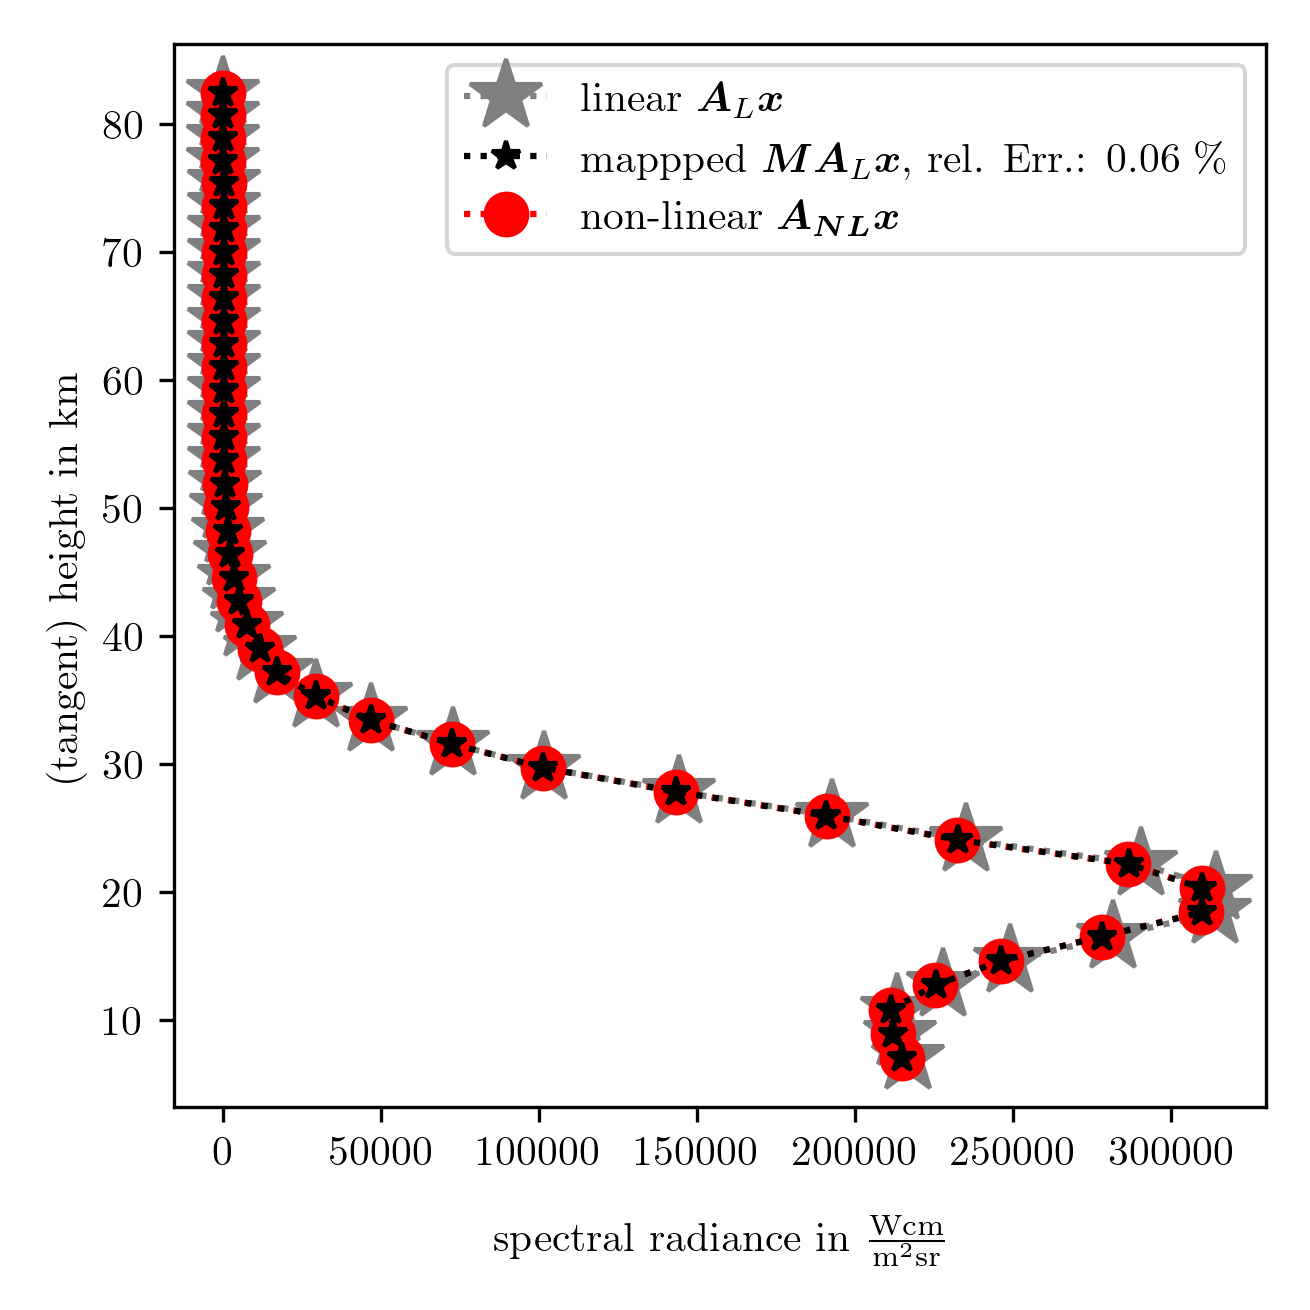
\includegraphics{SampMapAssesment.png}
	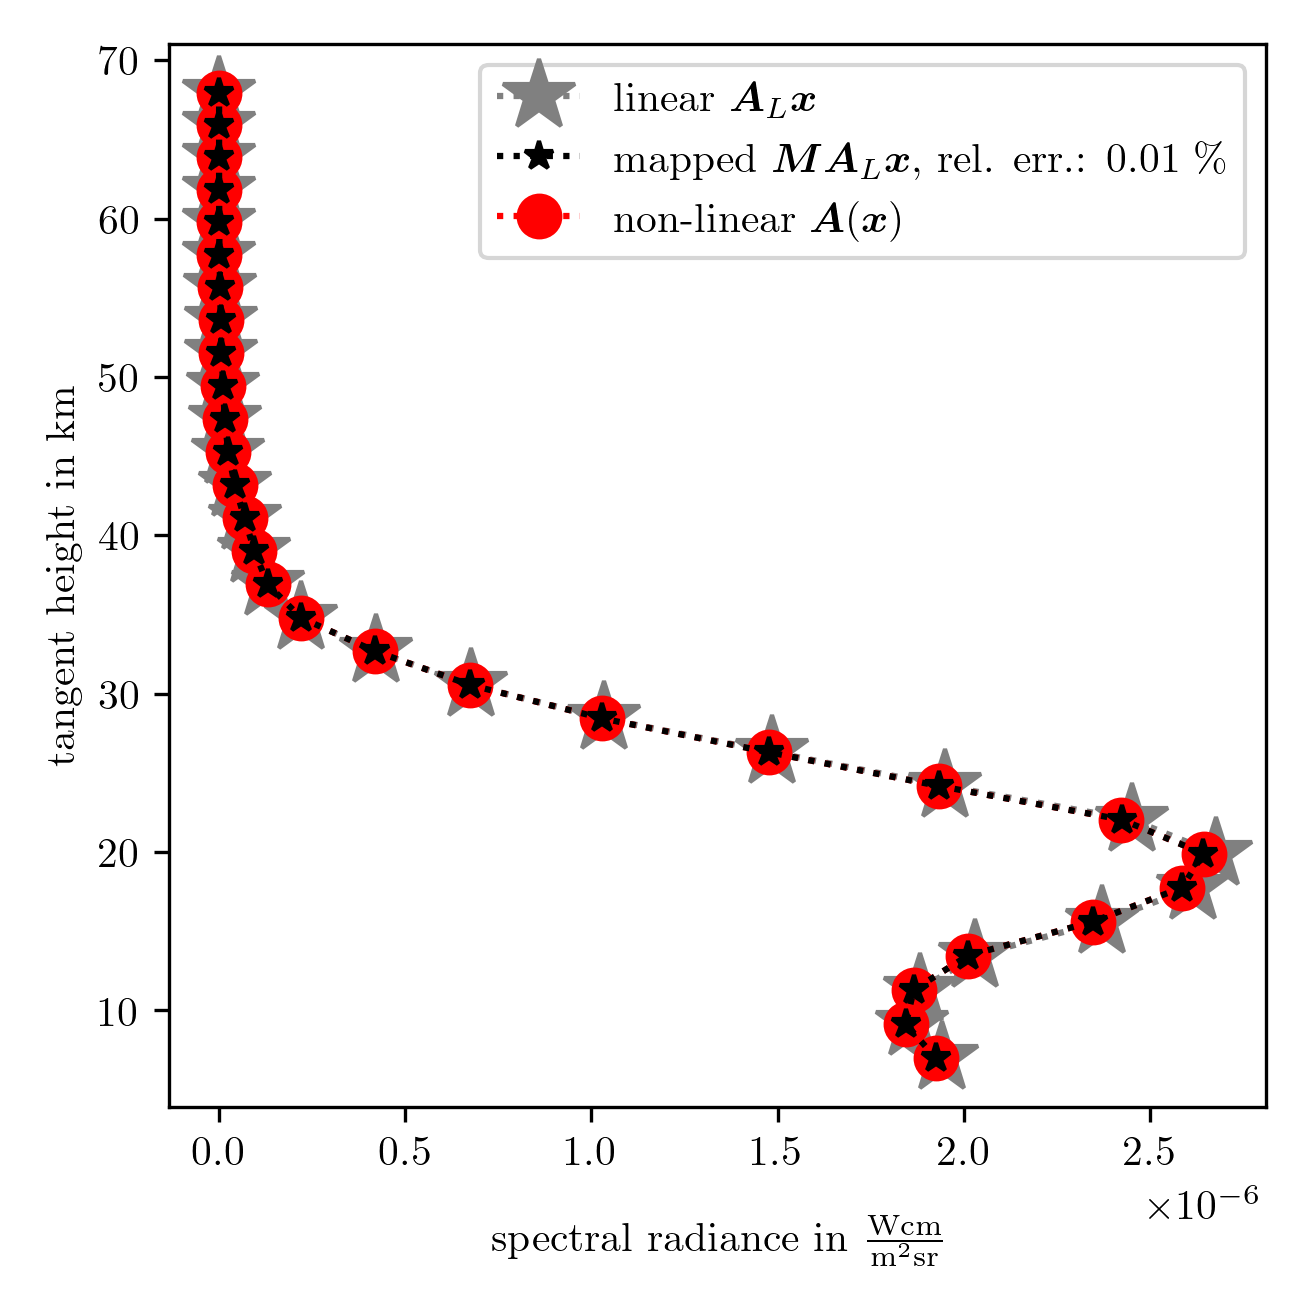
\includegraphics{SampMapAssesmentTT.png}
	\caption[Assessment of affine map.]{We asses how good we can map a new ozone sample $\bm{x} \sim \pi(\bm{x}|\bm{y})$ from the linear forward model onto the non-linear forward model using the previous calculated affine map $\bm{M}$. The sample has not been used to create this affine map. The gray stars represent noise free linear data, where as the red circles present noise free non-linear data. Then we map the linear noise free data onto the non-linear noise free data, black start, and provide the relative RMS error in between the mapped noise free data and the non-linear data.}
	\label{fig:MapAsses}
\end{figure}
In Fig. \ref{fig:MapAsses}, we show the mapping for one posterior ozone sample which has not been used to create this mapping.
In other word this is an unseen event not in the training data.
The relative RMS error for this approximation is roughly $0.03\%$ and much smaller than the relative difference between noise free linear data and non-linear data.
Consequently, from here onwards, we use the approximated forward map and define $\bm{A} \coloneqq \bm{M A}_L $.
\clearpage

\section{Regularisation Solution vs. Bayesian Approach -- approximated Model}
%\section{Posterior Distribution of Ozone -- approximated Model}
With the affine approximation we define
\begin{align}
	\bm{A}  \coloneqq \bm{M A}_L \, 
\end{align}
of the non-linear forward map, we use the same setup as in Sec. \ref{sec:FirstO3Post} to evaluate the marginal posterior and the conditional posterior.
\subsection{Posterior Distribution for Ozone}

\subsubsection{Marginal Posterior}
The marginal posterior is defined as in Eq. \ref{eq:MargPostAppl}, but with updated forward model.
We initialise the MWG at the mode of $\pi(\gamma, \lambda | \bm{y})$ and approximate $f(\lambda)$ and $g(\lambda)$ around the mode as in Eq. \ref{eq:fAprox} and Eq. \ref{eq:gAprox}.
Then we run the MWG algorithm for $N = 10000$ plus $N_{\text{burn-in}} = 100$ steps and plot the samples in Fig. \ref{fig:MargPostHistTT} as well as the marginal approximations provided by the TT decomposition, where we use the exact same setup as in Sec. \ref{subsec:firstMargTT}.

\begin{figure}[ht!]
	\centering
	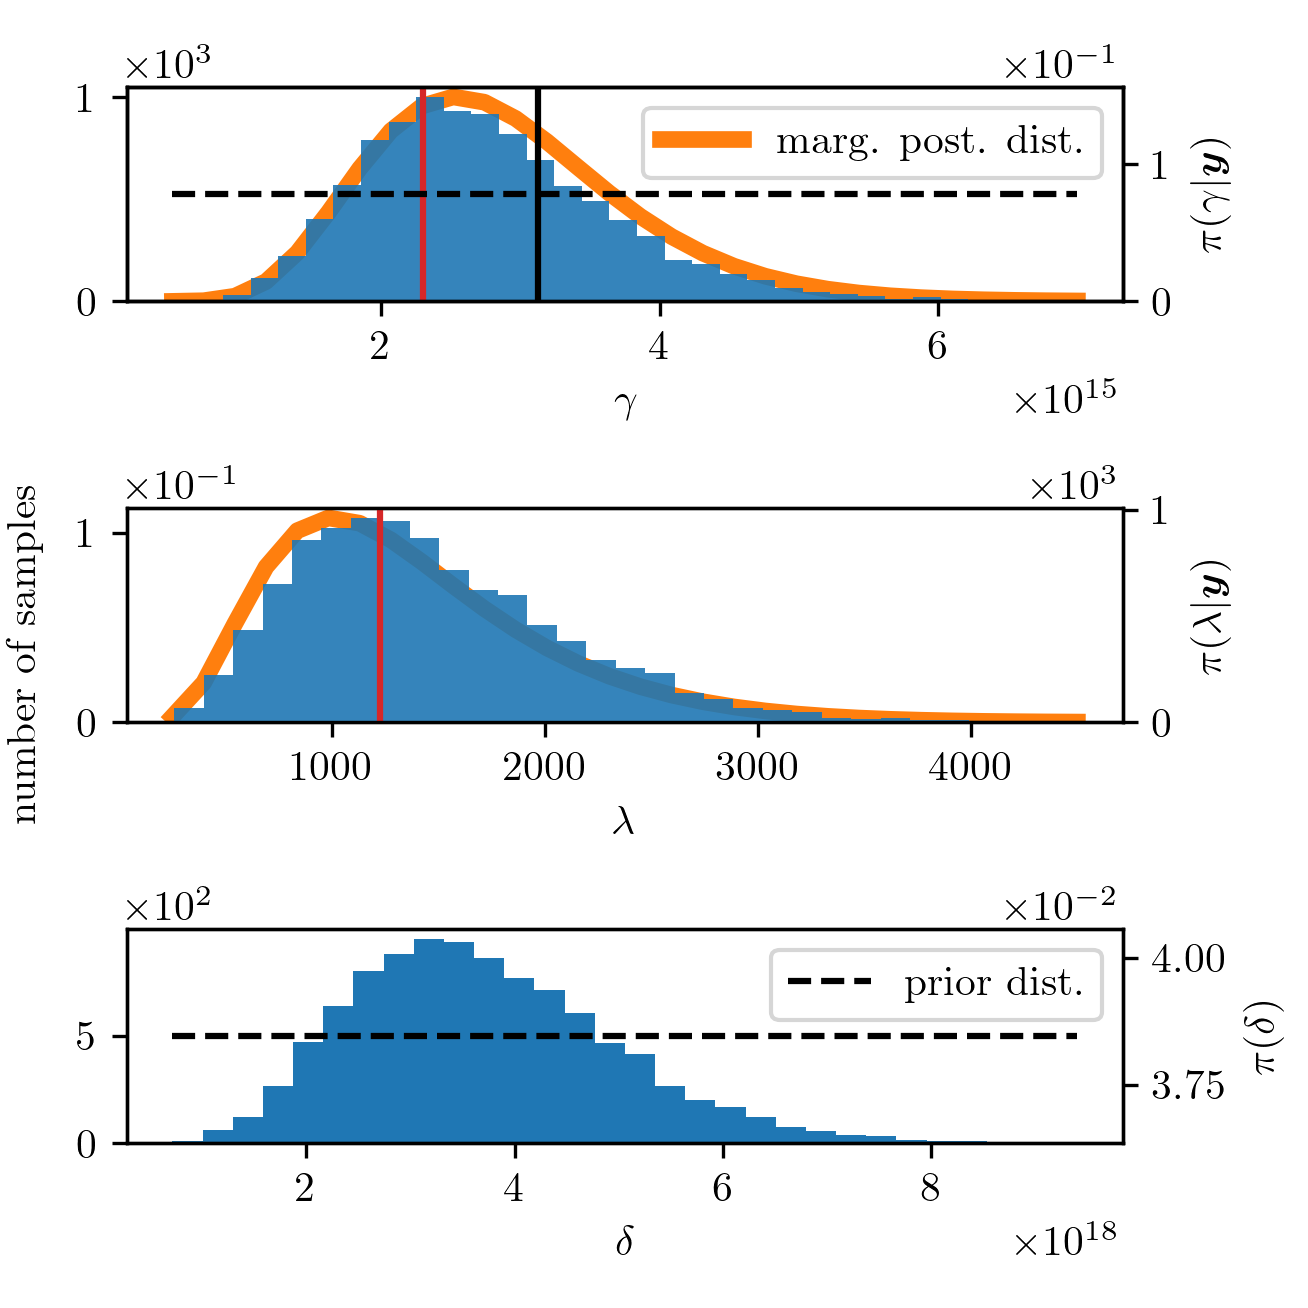
\includegraphics{secMargO3Res.png}
	\caption[Marginal posterior histograms and TT approximation as well as hyper-prior distribution.]{We plot the TT approximation of marginal posterior in orange and the samples as a histogram as well as the prior distribution with a dotted line. Note that we sample $\lambda$ and $\gamma$ using the Metropolis-within-Gibbs sampler and can calculate $\delta$ for every sample of the marginal posterior, we can not do this for the TT approximation. The regularised parameter corresponding to the regularised solution is marked thought the red vertical line at $\lambda_{\text{reg}} =$.}
	\label{fig:MargPostHistTT}
\end{figure}

\subsubsection{Full Posterior Variance and Mean}
Next, we characterise the conditional posterior $\pi(\bm{x}|\bm{y})$ as in Eq. \ref{eq:CondPost}. 
Again, we calculate the full posterior mean $\bm{\mu}_{\bm{x}|\bm{y}}$, see Eq. \ref{eq:MeanInt}, and covariance matrix $\bm{\Sigma}_{ \bm{x}|\bm{y}}$ \ref{eq:CovInt} as weighted expectation over a 20-point grid provided by either the marginal TT-approximations of $\pi(\gamma| \bm{y})$ and $\pi(\lambda| \bm{y})$ or by the bins of the sample histogram as quadrature weights.
We plot the conditional mean and variance in Fig. \ref{fig:O3SolplsReg}, the regularised solution, see next section, and one sample from the posterior, which represents a feasible solution to this inverse problem.
We can see that the ground truth lays within 3 times the variance around the mean accounting for roughly $99 \%$ of all solution, except for the peak at around $80$km.
We also note that compared to the previously calculated mean and variance based on the linear forward model, see \ref{fig:O3Samp}, the approximated based posterior distribution does not differ significantly.
This is expected since the $1\%$ difference between the linear and non-linear forward map is small.
\begin{figure}[ht!]
	\centering
	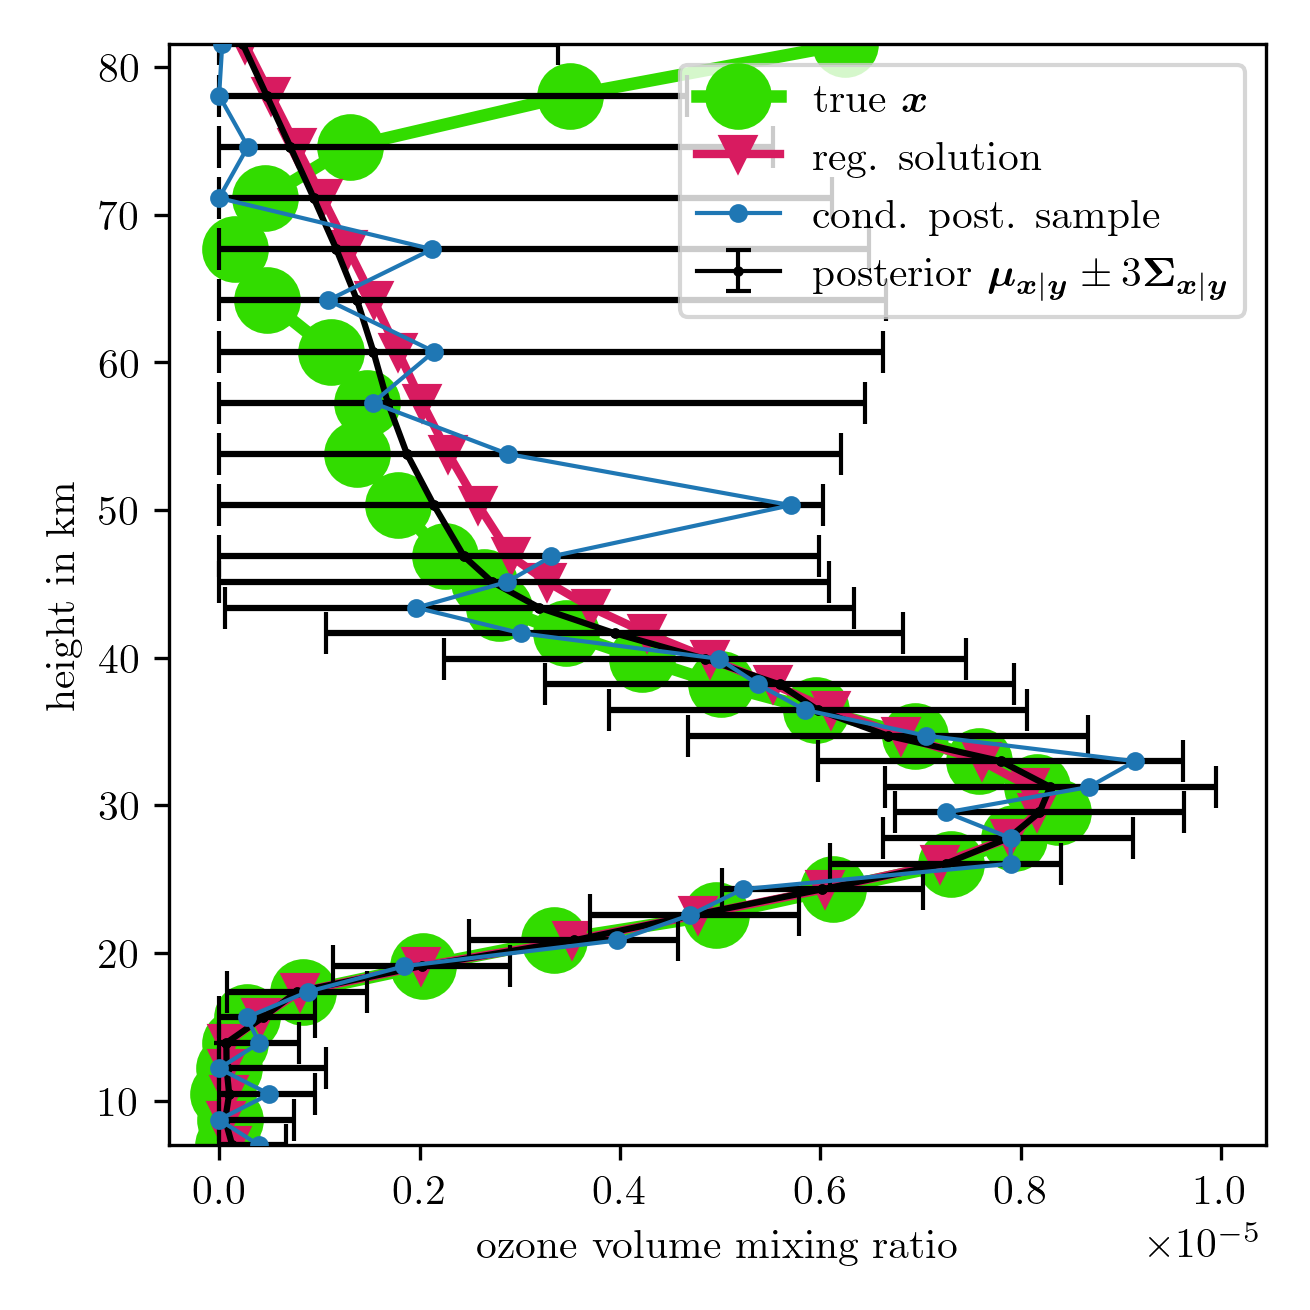
\includegraphics{SecRecResinclRegandSampl.png}
	%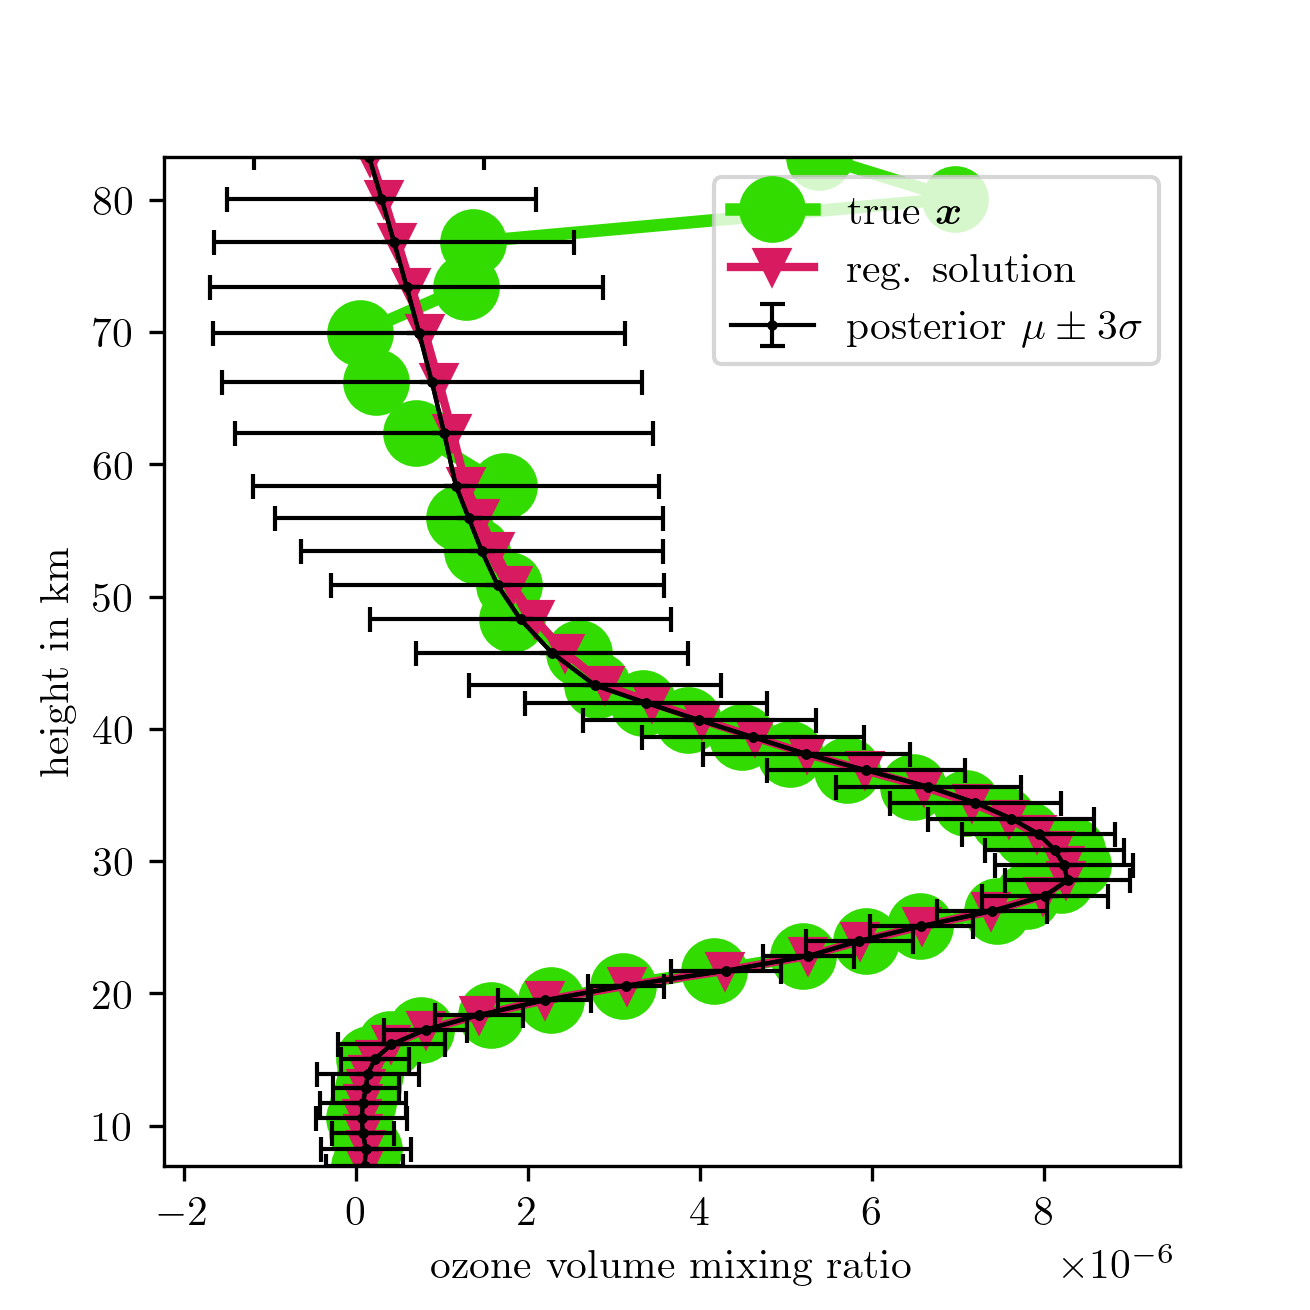
\includegraphics{SecRecResinclReg.png}
	\caption[Ozone posterior mean and variance and the regularised solution compared to the ground truth.]{We plot the conditional posterior mean and variance in black and the regularised solution on top of the ground truth ozone profile in green. We use the updated forward map $\bm{M}\bm{A}_L$}
	\label{fig:O3SolplsReg}
\end{figure}

Additionally in Fig. \ref{fig:PostCov}, we plot the singular values of the covariance matrix $\bm{\Sigma}_{ \bm{x}|\bm{y}}$, to visualise how many ozone values are informative.
We observe that the last 10 singular values are very small and correspond to ozone values at the high altitudes $\gtrsim 45$ with a large variance, see Fig. \ref{fig:O3SolplsReg}.
At those high altitudes the solution is dominated by the prior.
\begin{figure}[ht!]
	\centering
	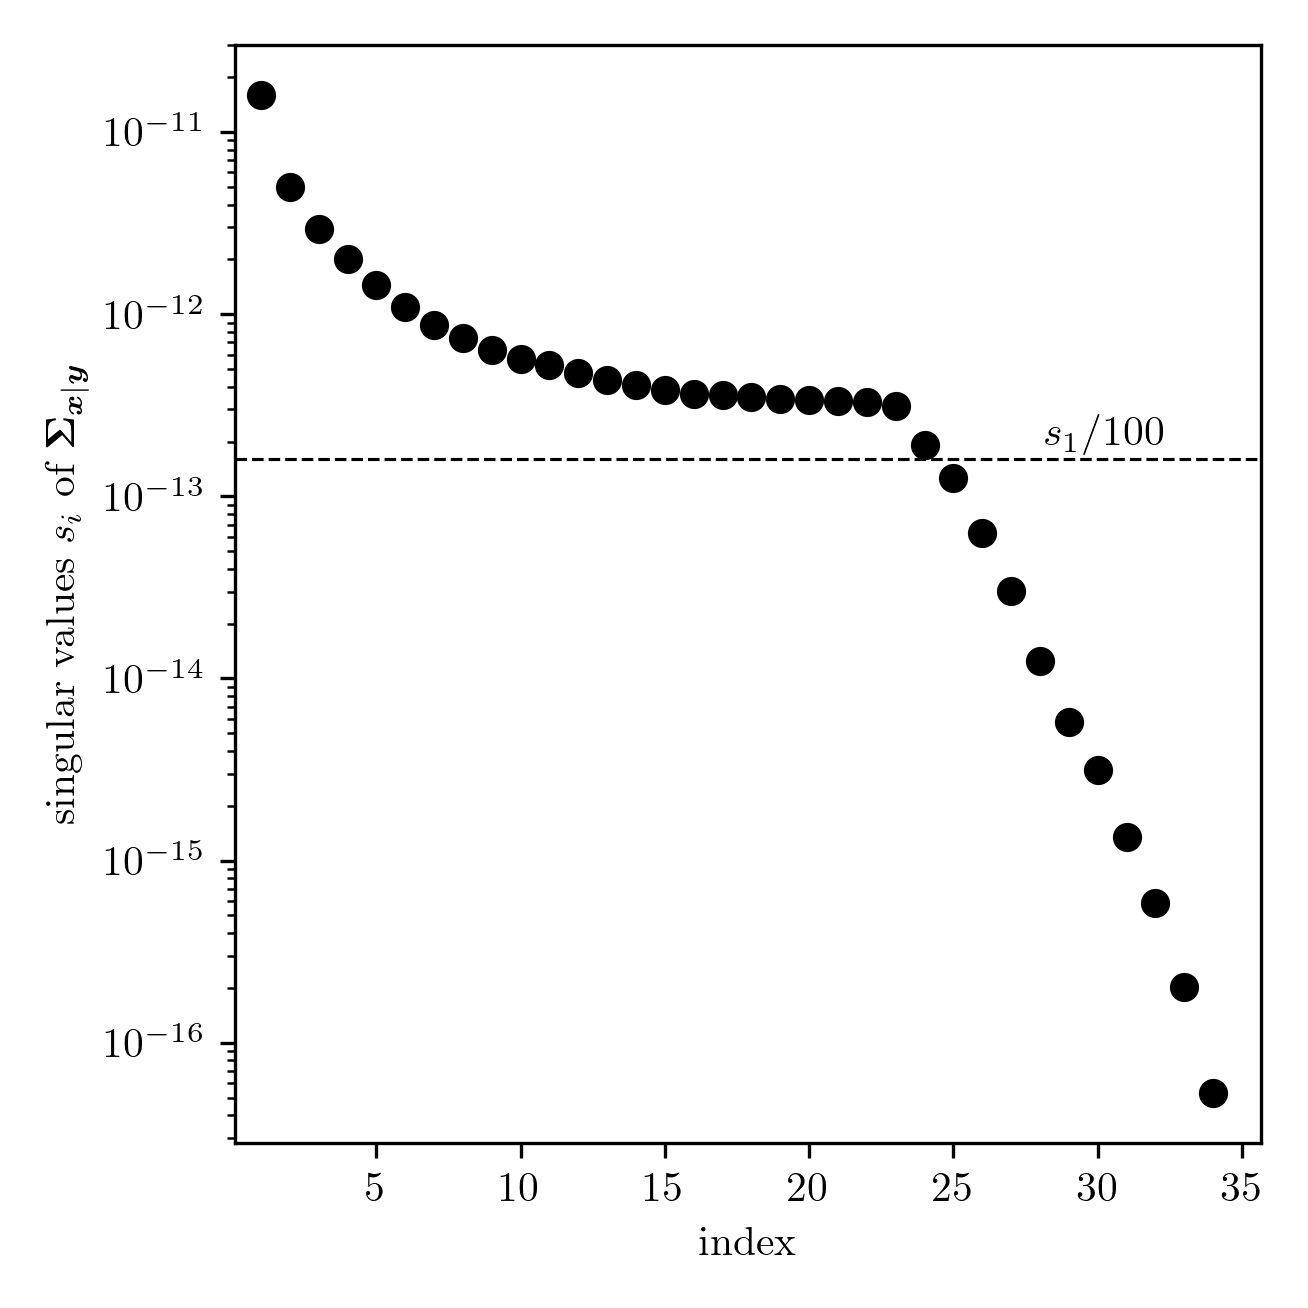
\includegraphics{CovSing.png}
	\caption[Singular values of the posterior covariance matrix]{Singular values of the covariance matrix of $\bm{\Sigma}_{ \bm{x}|\bm{y}}$ of the posterior distribution $\pi(\bm{x}|\bm{y})$ for ozone.}
	\label{fig:PostCov}
\end{figure}
\clearpage


\subsection{Solution by Regularisation}
\label{sec:reg}
Since we claim that Bayesian analysis is superior to regularisation methods we compare the MTC method to a Tikhonov regularisation solution, see Sec. \ref{sec:regularise} and \cite{fox2016fast}.
This is most similar to our chosen linear-Gaussian Bayesian framework.
The Tikhonov regularised solution is defined as in~\cite{hansen2010discrete, fox2016fast} 
\begin{align}
	\bm{x}_{\lambda} =\underset{ \bm{x}}{\arg \min}\,  \lVert \bm{A}\bm{x} - \bm{y} \rVert_2^2 + \lambda \bm{x}^T \bm{L} \bm{x} \, ,
	\label{eq:XLam}
\end{align}
with the regularisation parameter $\lambda$.
The regularised solution is typically calculated by solving the normal equations, see Sec. \ref{sec:regularise},
\begin{align}
	\bm{x}_{\lambda} = (\bm{A}^T\bm{A} + \lambda \bm{L} )^{-1} \bm{A}^T \bm{y} \label{eq:xLam} \, .
\end{align}
To find the best regularised solution, we use the L-curve method~\cite{hansen1993use}.
Within this method we compute $\bm{x}_\lambda$, for 200 different $\lambda$ values in between $1$ to $10^7$ and plot the solution semi norm $\sqrt{\bm{x}_\lambda^T\mathbf{L} \bm{x}_\lambda}$ against the data misfit norm $\lVert \bm{A}\bm{x}_\lambda - \bm{x} \rVert$, see Figure \ref{fig:LCurve}. 
The best regularised solution corresponding to the corner of the L-curve is located at the point of maximum curvature, see triangle in Fig. \ref{fig:LCurve}, which we find with the kneedle algorithm~\cite{satopaa2011kneedle} using the python function \texttt{kneed.KneeLocator} in less $0.1$s.
\begin{figure}[ht!]
	\centering
	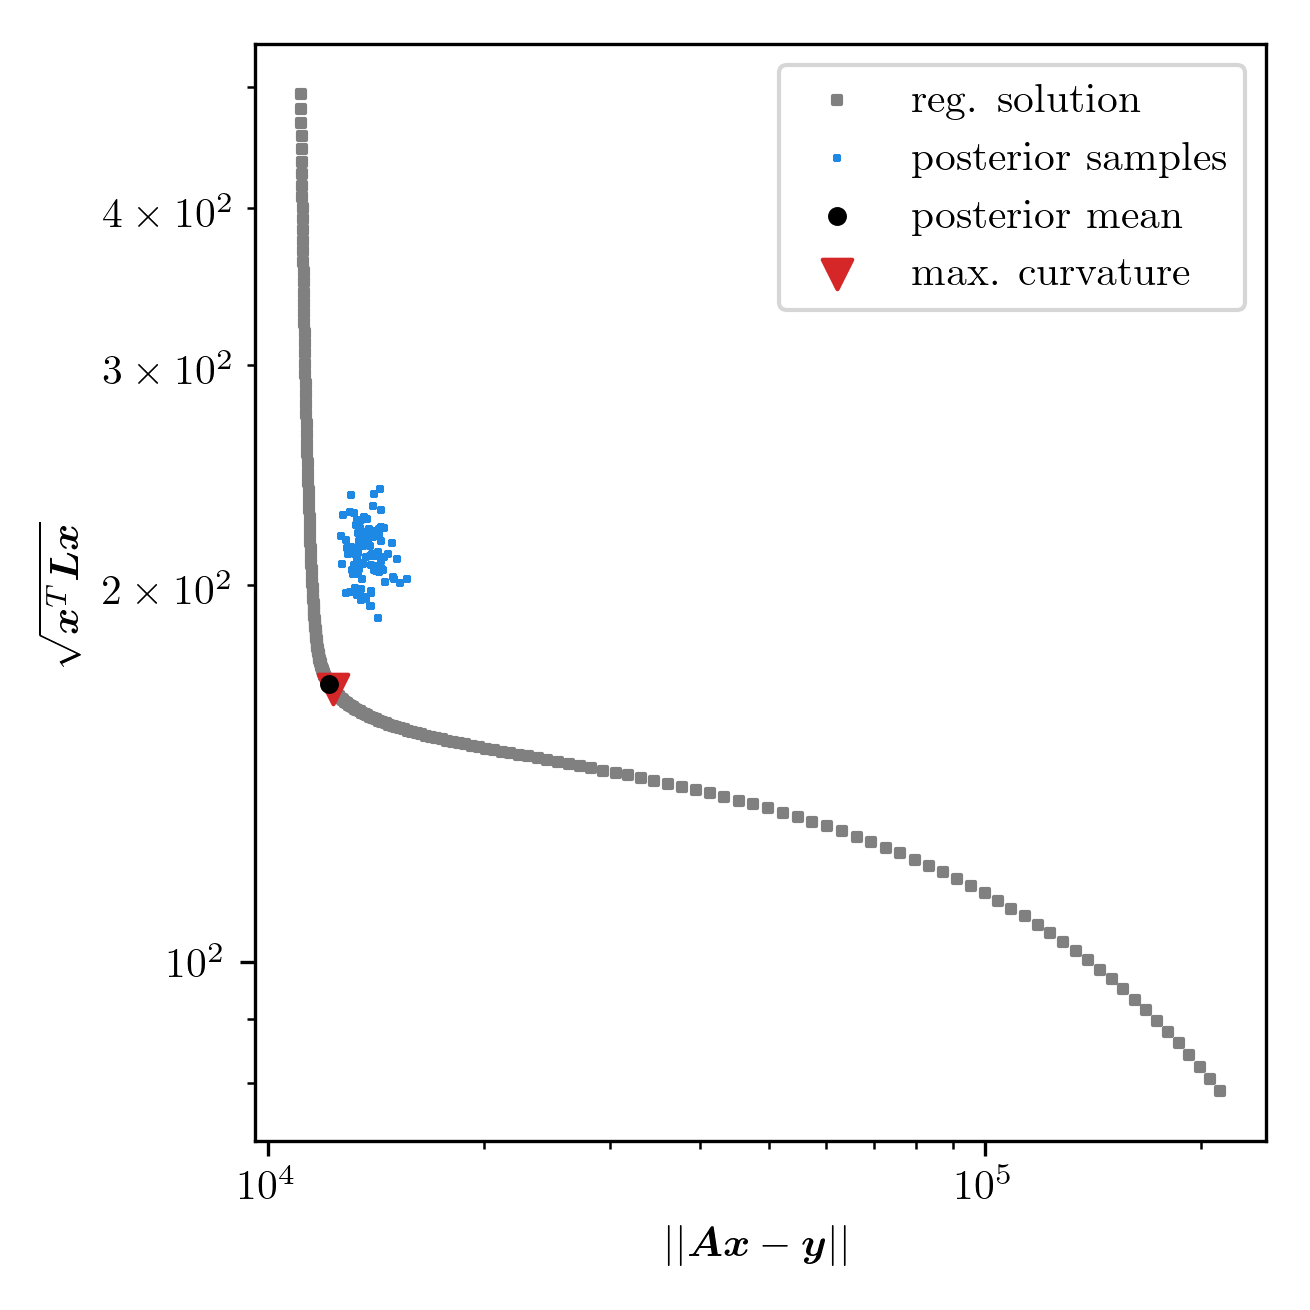
\includegraphics{LCurvePhD.png}
	\caption[Plot of the L-curve to find the regularised solution.]{We calculate regularised solution as in Eq. \ref{eq:} and plot the regularised semi norm $\sqrt{\bm{x}^T\bm{Lx}}$ against the data misfit norm $||\bm{Ax} -\bm{y} ||$ to find the regularised solution at the point of maximum curvature of the so-called L-Curve. Additionally we calculate the data misfit norm and the regularised norm for the ozone posterior and for samples of the conditional posterior distribution. \textcolor{red}{make box around Kneedle reagion}}
	\label{fig:LCurve}
\end{figure}

We plot the regularised solution in Fig. \ref{fig:O3SolplsReg} and observe that it is very similar to the posterior mean.
It is pretty clear that the regularised solution accounts for only one possible solution and does not provide uncertainties. The regularised solution is not similar to the samples drawn from the posterior $\pi(\bm{x}| \bm{y})$, see also Fig. \ref{fig:O3Samp}.
In Fig. \ref{fig:LCurve}, the samples of $\pi(\bm{x}| \bm{y})$ lie above the L-Curve where as the mean and the regularised solution lie on the L-Curve.
This does make sense, if one thinks about the mean (average over less smooth samples) and the regularised solution as extremely smooth ozone profiles, see also Sec. \ref{sec:regularise}.
In contrast the samples are less regularised and hence lie above the L-Curve, but have a similar data misfit norm and as already mentioned are all feasible solution to the data.
Neither the regularisation solution nor the posterior ozone profiles capture the ozone peak of the ground truth at high altitudes.
\clearpage

\section{Hierarchical Bayesian Framework for Ozone, Pressure and Temperature}
\begin{figure}[thb!]
	\centering
	\begin{tikzpicture}
		\node[roundnode2] at (-4.5,6.5) (Q)     {$\bm{Q}$};
		\node[roundnode2] at (-3,5) (x)     {$\bm{x}$};
		\node[align=center] at (-1,4) (A)    {$\bm{A} \coloneqq  \bm{M}\bm{A}_L$};
		\node[roundnode2] at (-1,2.5) (u)    {$\Omega$};
		\node[rectnode] at (-1,1) (y)    {$\bm{y}$};
		\node[roundnode2] at (-2.5,2.5) (e)    {$\bm{\eta}$};
		\node[roundnode2] at (-6.25,6.5) (S)    {$\bm{\Sigma}$};
		\node[roundnode2] at (-7.75,8) (s)    {$\gamma$};
		\node[roundnode2] at (-6,8) (d)    {$\delta$};
		\node[roundnode2] at (3,6.5) (t)     {$\bm{T}$};
		\node[roundnode2] at (-1,6.5) (p)     {$\bm{p}$};
		\node[roundnode2] at (1,5) (pt)     {$\bm{p}/\bm{T}$};
		\node[roundnode2] at (0,8) (b1)    {$b$};
		%\node[roundnode2] at (1,8) (b2)    {$b_2$};
		%\node[roundnode2] at (-2,8) (h1)    {$h_{0}$};
		\node[roundnode2] at (-1.5,8) (p0)    {$p_0$};
		\node[roundnode2] at (2.25,8) (ht)    {$\bm{h_T}$};
		\node[roundnode2] at (3.25,8) (ct)    {$T_0$};
		\node[roundnode2] at (4.25,8) (at)    {$\bm{a}$};
		
		\node[roundnode2] at (0,10) (b1hyp)    {$\bm{\theta}_{b}$};
		%\node[roundnode2] at (-2.5,10) (h1hyp)    {$\bm{\theta}_{h_{0}}$};
		\node[roundnode2] at (-1.5,10) (p0hyp)    {$\bm{\theta}_{p_{0}}$};
		\node[roundnode2] at (2,10) (hthyp)    {$\bm{\theta}_{\bm{h}_T}$};
		\node[roundnode2] at (3.25,10) (cthyp)    {$\bm{\theta}_{T_{0}}$};
		\node[roundnode2] at (4.5,10) (athyp)    {$\bm{\theta}_{\bm{a}}$};
		
		\node[roundnode2] at (-7.75,10) (shyp)    {$\bm{\theta}_{\gamma}$};
		\node[roundnode2] at (-6,10) (dhyp)    {$\bm{\theta}_{\delta}$};
		
		%Lines
		
		
		\draw[->, very thick] (S) -- (e);
		\draw[->, mydotted, very thick] (s) -- (S);
		\draw[->, very thick] (u) -- (y);
		\draw[->, mydotted, very thick] (A) -- (u);
		\draw[->, mydotted,  very thick] (x) -- (A.north west);
		\draw[->, mydotted, very thick] (p) -- (pt);
		\draw[->, mydotted, very thick] (t) -- (pt);
		\draw[->, mydotted, very thick] (pt) -- (A.north east);
		%\draw[->, mydotted, very thick] (h1) -- (p);
		\draw[->, mydotted, very thick] (p0) -- (p);
		\draw[->, mydotted, very thick] (b1) -- (p); 
		%\draw[->, very thick] (b2.south) -- (p.east); 
		\draw[->, mydotted, very thick] (d) -- (Q); 
		\draw[->, mydotted, very thick] (e) -- (y); 
		
		\draw[->, very thick] (Q.south east) -- (x.north west); 
		\draw[->, mydotted, very thick] (ht.south) -- (t.north west);
		\draw[->, mydotted, very thick] (ct.south) -- (t.north);
		\draw[->, mydotted, very thick] (at.south) -- (t.north east);
		
		
		\draw[->, very thick] (b1hyp) -- (b1);
		%\draw[->, very thick] (h1hyp) -- (h1);
		\draw[->, very thick] (p0hyp) -- (p0);
		\draw[->, very thick] (hthyp) -- (ht);
		\draw[->, very thick] (cthyp) -- (ct);
		\draw[->, very thick] (athyp) -- (at);
		\draw[->, very thick] (shyp) -- (s);
		\draw[->, very thick] (dhyp) -- (d);
		
		\node[fit=(s)(at),draw,dotted,black, rounded corners] {};
		\node[align =center] at (-3.75,8) (T1) {hyper-parameters};
		
	\end{tikzpicture} 
	\caption[Complete directed acyclic graph of the forward model.]{Complete directed acyclic graph (DAG) of the forward model. The hyper-parameters at the top deterministically (dotted line) describe the parameters ($\bm{p}/\bm{T}$) or the noise covariance $\bm{\Sigma} = \gamma^{-1} \bm{I}$ of the random (solid line) noise $\bm{\eta} \sim \mathcal{N}(0,\gamma^{-1} \bm{I} ) $ and precision matrix $\bm{Q} = \delta \bm{L}$ of the distribution of $\bm{x}\sim \mathcal{N}(0,\delta \bm{L}) $, where $\bm{L}$ is a graph Laplacian as in Eq. \ref{eq:GLapl}. We can group the noise precision $\gamma$  and the smoothness parameter $\delta$ to define the marginal posterior over those hyper-parameters and then condition on them for the conditional posterior distribution,for further details see Fig. \ref{fig:DAGO3}. In this whole process where we condition on the pressure $\bm{p}$ and temperature $\bm{T}$, which we retrieve separately, see Fig. \ref{fig:DAGPT}. The hyper-parameters $h_0,p_0,b$ deterministically describe the pressure function in Eq. \ref{eq:pressFunc}, note that we only need three parameters here since $h_0< h_{L,0}$ and $\bm{h}= \{ h_1, h_2,h_3,h_4,h_5,h_6\}$, $\bm{a} = \{ a_0, a_1, a_2,a_3,a_4\}$ and $T_0$ determine the temperature function.
		The parameters $\bm{x}$ and $\bm{p}/ \bm{T}$ determine the space of all measurable noise free data $\bm{\Omega}$ through the forward model $\bm{A}(\bm{x},\bm{p},\bm{T})$ from which we randomly observe data set plus some random noise.}
	\label{fig:DAGComplete}
\end{figure}

A directed acyclic graph (DAG) helps us to visualise the measurement process and correlations between parameters.
We draw a DAG in Fig. \ref{fig:DAGComplete} and already see that the parameters pressure $\bm{p}$, temperature $\bm{T}$ and ozone $\bm{x}$ are correlated, and progress deterministically (dashed line) into the forward model, via $\bm{x} \times \bm{p} / \bm{T}$ and generate a space of all possible noise free data $\bm{\Omega}$, through their respective prior distributions, from which we observe some data.
Ideally, we should infer all of them jointly, but that is computationally very expensive.
Instead, we condition on either ozone when inferring pressure and temperature or on pressure and temperature when inferring ozone.
Then one should iteratively proceed until convergence, but this is not the focus of this thesis since we provide the underlying Bayesian framework and methods to obtain posterior distributions of either one and suggest adjustments to the proposed framework in Ch. \ref{ch:Concl}.
Since we consider a hierarchical Bayesian framework, we include the hyper-parameters $\gamma, \delta, p_0, b, \bm{h}_T, \bm{T}_0, \bm{a}$ within the modelling process.
Here pressure and temperature are functionally dependent on $p_0, b, \bm{h}_T, \bm{T}_0, \bm{a}$, see Eq. \ref{eq:tempFunc} and Eq. \ref{eq:pressFunc}, visualised through dashed lines, but $\delta$, accounting for the smoothness of $\bm{x}$, determines the precision matrix $\bm{Q}$ of the prior distribution $\pi(\bm{x}|\delta)$, which then represents a distribution over non-parametric $\bm{x}$ (solid line).
Similarly, $\gamma$ determines the noise covariance matrix $\bm{\Sigma}$, which then describes the noise vector as $\eta \sim \mathcal{N}( \bm{0}| \gamma^{-1} \bm{I})$, where we assume independent and identically distributed normal noise with zero mean.
Each of those hyper-parameters is described by hyper-prior distributions $\pi(\gamma, \delta, p_0, b, \bm{h}_T, \bm{T}_0, \bm{a} |\theta_{\gamma}, \theta_{\delta},\theta_{p_0},\theta_{b},\theta_{\bm{h}},\theta_{T_0},\theta_{\bm{a}} )$ (solid lines).
Here $\theta_{\gamma}, \theta_{\delta},\theta_{p_0},\theta_{b},\theta_{\bm{h}},\theta_{T_0},\theta_{\bm{a}}$ are set by us and determine in this case gamma distributions $\gamma, \delta \sim \pi(\theta_{\gamma}, \theta_{\delta})$, so that e.g. $\gamma \sim \Gamma(\alpha_{\gamma},\beta_{\gamma}) $ with $\theta_{\gamma} = \{\alpha_{\gamma},\beta_{\gamma} \}$, and a normal distribution $p_0, b, \bm{h}_T, \bm{T}_0, \bm{a} \sim \pi( \theta_{p_0},\theta_{b},\theta_{\bm{h}},\theta_{T_0},\theta_{\bm{a}})$, so that e.g. $b \sim \mathcal{N}(\mu_b, \sigma_b)$ and $\theta_{b} = \{\mu_b, \sigma_b\}$
Note that we write the non-linear forward model, with which we generate the data as $\bm{A}_{NL}$, but denote the approximated forward model as $\bm{M} \bm{A}_L$, which we will ultimately use to determine the posterior distribution over the parameters.


Since the noise is normally distributed, so is the likelihood function $\pi(\bm{y} | \bm{x}, \bm{p}, \bm{T})$.
Then the joint posterior distribution
\begin{align}
	\pi(p_0,b,\bm{h_T},\bm{a},\delta, \gamma, \bm{x}| \bm{y}) \propto \pi(\bm{y} | \bm{x}, \bm{p}, \bm{T}) \pi(p_0,b,\bm{h_T},\bm{a},\delta, \gamma) 
\end{align}
over all 18 hyper-parameters and the parameter $\bm{x} \in \mathbb{R}^{45}$ is 63 dimensional.
Instead of characterising the joint posterior, we factorise the posterior into
\begin{align}
	\pi(p_0,b,\bm{h_T},\bm{a},\delta, \gamma, \bm{x}| \bm{y}) = \pi(\delta, \gamma, \bm{x}| p_0,b,\bm{h_T},\bm{a},\bm{y}) \pi(p_0,b,\bm{h_T},\bm{a}|\delta, \gamma, \bm{x}, \bm{y}) \, , 
\end{align}
where we either condition on ozone $\bm{x}$ and the smoothness hyper-parameter $\delta$ as well as the noise hyper-parameter $\gamma$ or on the fraction $\bm{p}/\bm{T}$, pressure over temperature, and its hyper-parameters.
Again, as in Sec. \ref{ch:formodel}, for brevity we write $\pi(\delta, \gamma, \bm{x}|\bm{y})$ for $\pi(\delta, \gamma, \bm{x}|p_0,b,\bm{h_T},\bm{a},\bm{y})$, which implies that we conditioned on $\bm{p}$ and $\bm{T}$. 
Next, we need to make prior assumptions about the parameters and to specify the prior and hyper-prior distributions, which we summarise in Tab. \ref{tab:priors}, and to formulate the posterior distributions.
\begin{table}
	\centering
	\begin{tabular}{ |c||c|c|c|c|c|   }
		\hline
		& &\multicolumn{2}{|c|}{TT bounds}& &\\
		\hline
		model parameters& priors&\makecell{lower}& \makecell{upper\\
		}&$\tau_{\text{int}}$&Context\\
		\hhline{|=||=|=|=|=|=|}
		$\gamma$ & $\mathcal{T}(1,10^{-10})$ &$5 \, 10^{-8}$ &$4.5 \, 10^{-7}$&  $ 9\pm 0.1$ &$\bm{y}$\\ \hline
		$\delta$ &$\mathcal{T}(1,10^{-10})$ & -&-& $1.5 \pm 0.1$ & $\bm{x}$\\ \hline
		$\lambda  = \delta / \gamma$ &- & 500&$10^4$& $3.5 \pm 0.3$ &$\bm{x}$\\ \hline
		$\bm{x}$ &$\mathcal{N}(0,\delta \bm{L})$ & -&-&-& $\bm{x}$\\ \hhline{|=||=|=|=|=|=|}
		$p_0$ &  $\mathcal{N}(1243,5)$&1229 &1259&$550 \pm 9$&$\bm{p/T}$\\ \hline
		$T_{0}$ &  $\mathcal{N}(288.15,4.5)$& 275 &302&$2446 \pm 76$&$\bm{p/T}$\\ \hline
		$h_{T,1}$ &  $\mathcal{N}(11,0.5)$&9.5 &12.5&$1820 \pm 49$ &$\bm{p/T}$\\ \hline
		$b$ &  $\mathcal{N}(0.167,5\,10^{-4})$& 0.165& 0.171 &$2813 \pm 92$&$\bm{p/T}$\\ \hline
		$h_{T,3}$ &  $\mathcal{N}(32.3,2.5)$&25.2&39.8&$394 \pm 5$&$\bm{p/T}$\\ \hline
		$a_{0}$ &  $\mathcal{N}(-6.5,0.01)$&-6.53 &-6.47&$330 \pm 4$&$\bm{p/T}$\\ \hline
		$h_{T,2}$ &  $\mathcal{N}(20.1,1.6)$&17.7 &22.3&$454 \pm 7$&$\bm{p/T}$\\ \hline
		$a_{1}$ &  $\mathcal{N}(0,0.1)$&-0.3 &0.3&$508 \pm 8$&$\bm{p/T}$\\ \hline
		$a_{2}$ &  $\mathcal{N}(1,0.01)$&0.97 &1.03&$341 \pm 5$&$\bm{p/T}$\\ \hline
		$a_{3}$ &  $\mathcal{N}(2.8,0.1)$&2.5 &3.1&$316 \pm 4$&$\bm{p/T}$\\ \hline
		$h_{T,4}$ &  $\mathcal{N}(47.4,5)$&45.9 &48.9&$324 \pm 4$&$\bm{p/T}$\\ \hline
		$a_{4}$ &  $\mathcal{N}(0,0.1)$&-0.3 &0.3&$335 \pm 4$&$\bm{p/T}$\\ \hline
		$h_{T,5}$ &  $\mathcal{N}(51.4,5)$&49.9 &52.9&$319 \pm 4$&$\bm{p/T}$\\ \hline
		$a_{5}$ &  $\mathcal{N}(-2.8,0.1)$&-3.1 &-2.5&$335 \pm 4$&$\bm{p/T}$\\ \hline
		$h_{T,6}$ &  $\mathcal{N}(71.8,3)$&62.5 &80.8&$347 \pm 5$&$\bm{p/T}$\\ \hline
		$a_{6}$ & $\mathcal{N}(-2,0.01)$ &-2.03 &-1.97&$320 \pm 4$&$\bm{p/T}$\\
		\hline
	\end{tabular}
	\caption[Summary of relevant parameter characteristics, bounds and sampling statistics.]{Summary of relevant parameter characteristics, bounds and sampling statistics. We denote $\mathcal{N}(\mu,\sigma)$ as the Gaussian and $\mathcal{T}(\alpha = \text{scale}, \beta = \text{rate})$ as the gamma distribution. The IACT $\tau_{\text{int}}$ is estimated as in \cite{UwerrM} from posterior samples based on the approximated forward map.}
	\label{tab:priors}
\end{table}

Setting up a Bayesian model to determine the pressure and temperature posterior distribution, we observe that we can parametrise $\bm{p}$ and $\bm{T}$.
In doing so, we describe the pressure values in between $h_{L,0} \approx 7$km and $h_{L,n} \approx 82$km with an exponential function
\begin{align}
	p(h) =
	\exp \left( -b \, h \right)   \,  p_0 \quad ,h_{L,0}  \leq h \leq h_{L,n}
	\label{eq:pressFunc}
\end{align}
so that the pressure $\bm{p}$ is described through two hyper-parameters $p_0,b$, see Fig. \ref{fig:PriorPress}.
Similarly, the temperature as described in Eq. \ref{eq:tempFunc} can be parametrised with 14 hyper-parameters  $\bm{h}_T = \{ h_{T,1}, h_{T,2},h_{T,3},h_{T,4},h_{T,5},h_{T,6} \}$, $\bm{a} = \{a_0, a_1, a_2,a_3,a_4,a_5,a_6 \} $ and $T_0$, see Fig. \ref{fig:PriorTemp}.
Then, we set up the hierarchical Bayesian framework
\begin{subequations}
	\begin{align}
		\bm{y} |  \bm{p}, \bm{T}, \gamma &\sim \mathcal{N}(\bm{A} \, \bm{p}/\bm{T}, \gamma^{-1} \bm{I}) \label{eq:likelihoodPT} \\
		\bm{a}  &\sim \mathcal{N}(\bm{\mu}_{\bm{a}}, \bm{\Sigma}_{\bm{a}})\\
		\bm{h}_{\bm{T}}  &\sim \mathcal{N}(\bm{\mu}_{T}, \bm{\Sigma}_{\bm{h}_T}) \\
		T_0  &\sim \mathcal{N}(\mu_{T_0}, \sigma_{T_0} )\\
		p_0  &\sim \mathcal{N}(\mu_{p_0}, \sigma_{p_0} )\\
		b  &\sim \mathcal{N}(\mu_b, \sigma_b )
	\end{align}
	\label{eq:BayMode}
\end{subequations}
and define a normally distributed likelihood (due to Gaussian noise) and normally distributed priors, where the hyper-prior means and variances are described through $\bm{\theta}_{\bm{a}} =(\bm{\mu}_{\bm{a}}, \bm{\Sigma}_{\bm{a}})$, $\bm{\theta}_{\bm{h}_T} = (\bm{\mu}_{\bm{T}}, \bm{\Sigma}_{\bm{h}_T}) $, 
$\bm{\theta}_{T_0} = (\mu_{T_0}, \sigma_{T_0})$, $\bm{\theta}_{p_0} = (\mu_{p_0}, \sigma_{p_0})$, and $\bm{\theta}_{b} = (\mu_{b}, \sigma_{b})$, see DAG in Fig. \ref{fig:DAGComplete}.


\subsection{Prior Modelling}
To complete the model, we have to define a sensible hyper-prior distribution $\pi(\bm{h}_T, \bm{a}, T_0)$.
In doing so, we choose the variance and mean of the normally distributed hyper-prior distribution $\pi(\bm{h}_T)$ so that the temperature profile maintains its structure, $ h_{T, i} < h_{T, i+1}$ for $i = 1,\dots, 5$, see \ref{fig:HeightPriors}.
Further, we define $\pi(\bm{a})$ as normally distributed, because we find, through exploratory and prior analysis, see Fig. \ref{fig:PriorPressOverTemp}, that the data is uninformative about the temperature profile.
Similarly, we set $\pi(T_0)$ to a normal distribution so that it mimics a daily temperature variability of roughly 30K.
The hyper-prior distribution $\pi(p_0, b)$ for pressure-related hyper-parameters is also normally distributed.
We choose the variance for $\pi(p_0)$ so that $p_0$ has a variability of around 80hPa, close to what we can observe when looking at weather data.
Note that we fit one exponential function to ground truth pressure values between $h_{L,0} \approx 7$km and $h_{L,n} \approx 82$, so that the pressure values $p_0$ at sea level may be skewed due to that approximation.
To describe pressure values from sea level to $h_{L,0}$, we recommend using another exponential function with a different gradient.
We summarise the hyper-prior means and variances in Tab. \ref{tab:priors}.
\begin{figure}[ht!]
	\centering
	\input{TrueTemp.pdf_tex}
	%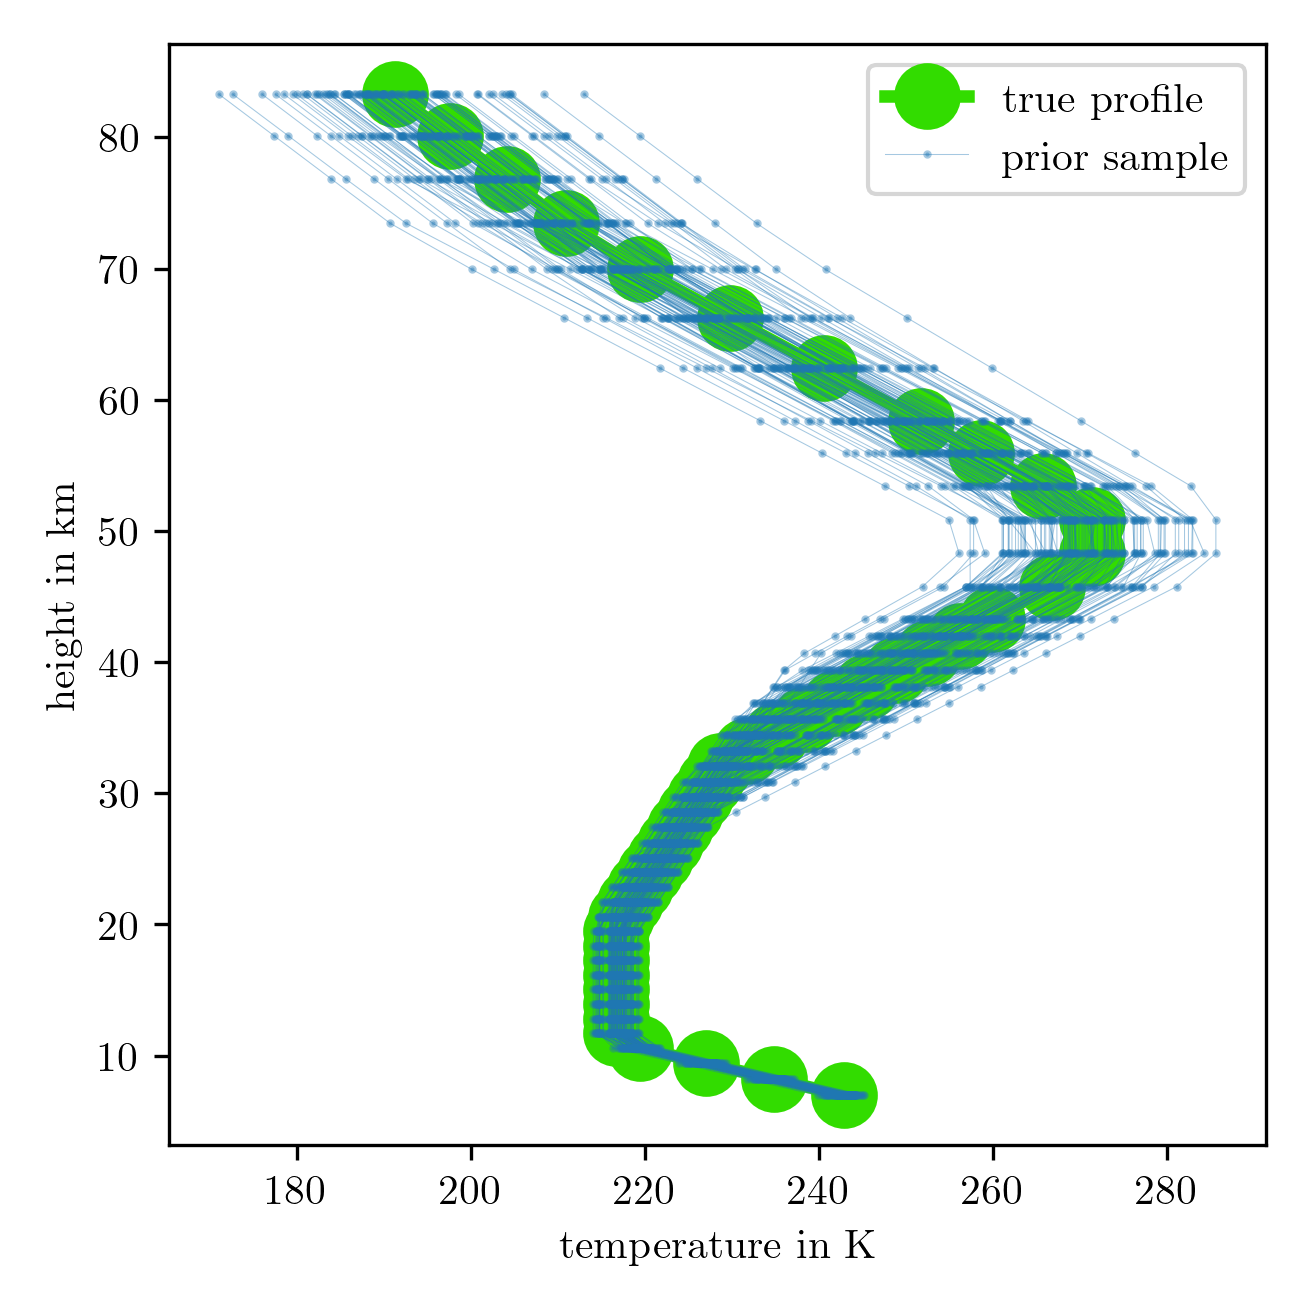
\includegraphics{PriorTempPostMeanSigm.png}
	\caption[Prior Samples of $\bm{T}$ according to the respective hyper-prior distribution.]{We draw samples from the hyper-prior distribution of $h_1, h_2,h_3,h_4,h_5,h_6, a_0, a_1, a_2,a_3,a_4$ and $T_0$ as defined in table \ref{tab:priors} and then calculate $\bm{T}$ according to the function in Eq. \ref{eq:tempFunc}.}
	\label{fig:PriorTemp}
\end{figure}

\begin{figure}[ht!]
	\centering
	\input{TruePress.pdf_tex}
	%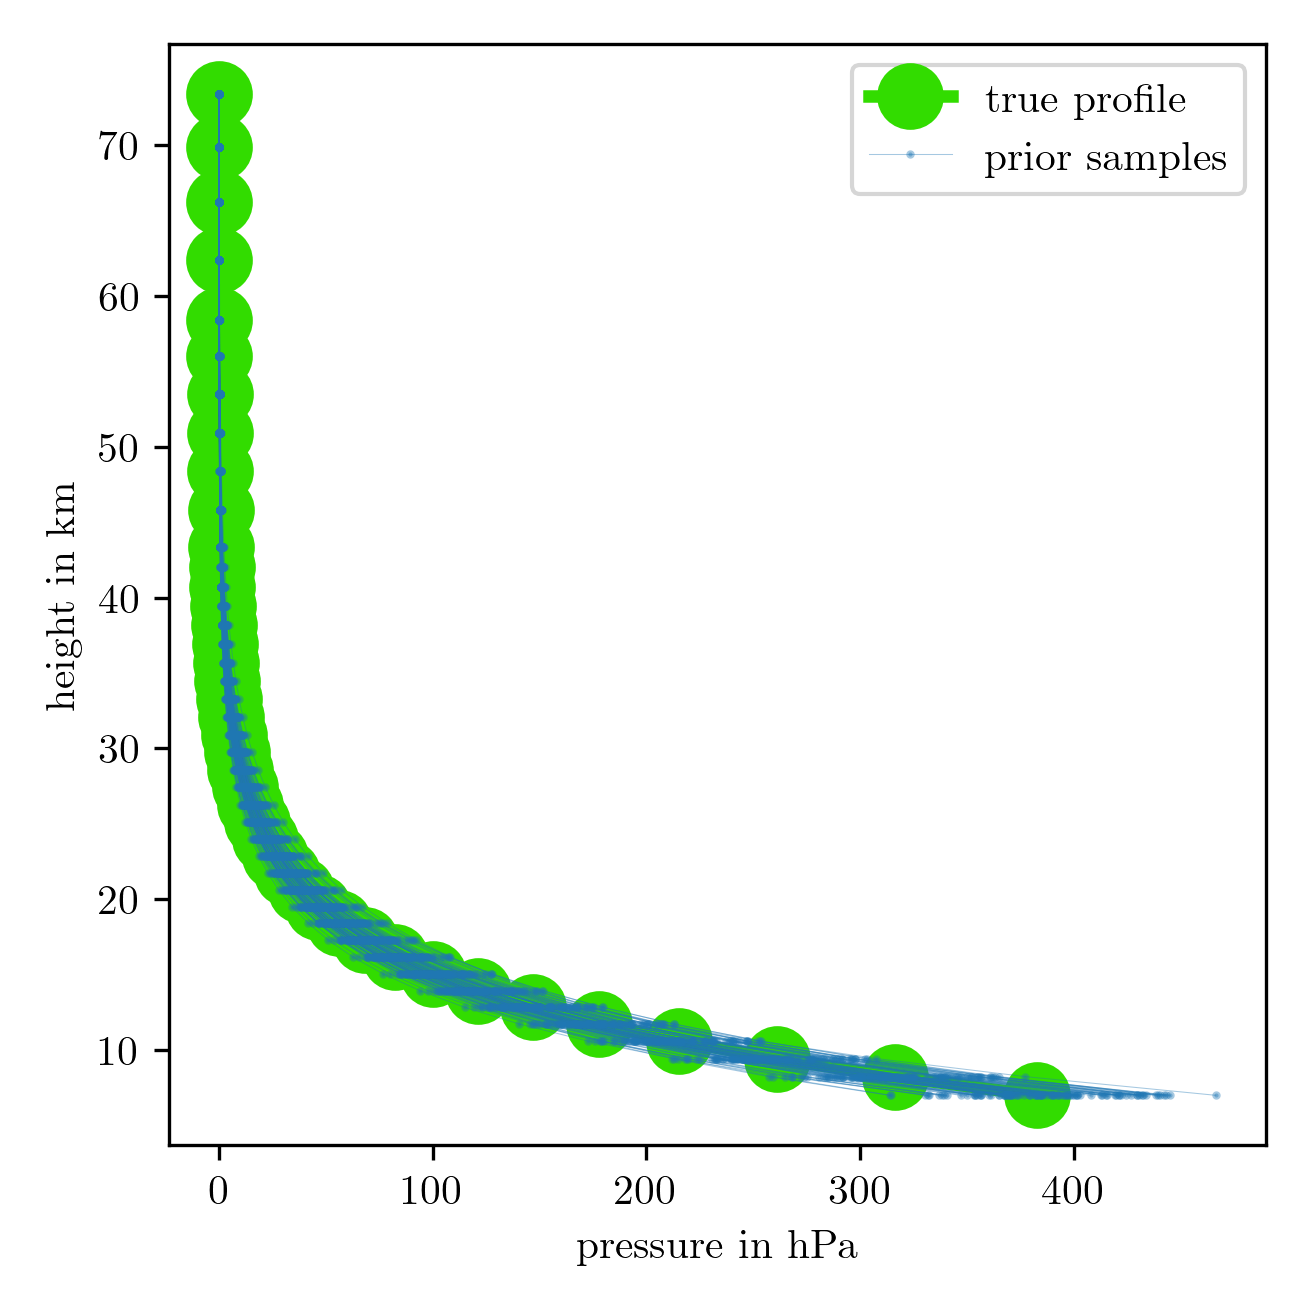
\includegraphics{PriorPressPostMeanSigm.png}
	\caption[Prior Samples of $\bm{p}$ according to the respective hyper-prior distribution.]{We draw samples from the hyper-prior distribution of $h_0, b$ and $p_0$ as defined in table \ref{tab:priors} and then calculate $\bm{p}$ according to the function in Eq. \ref{eq:pressFunc}.}
	\label{fig:PriorPress}
\end{figure}
\begin{figure}[ht!]
	\centering
	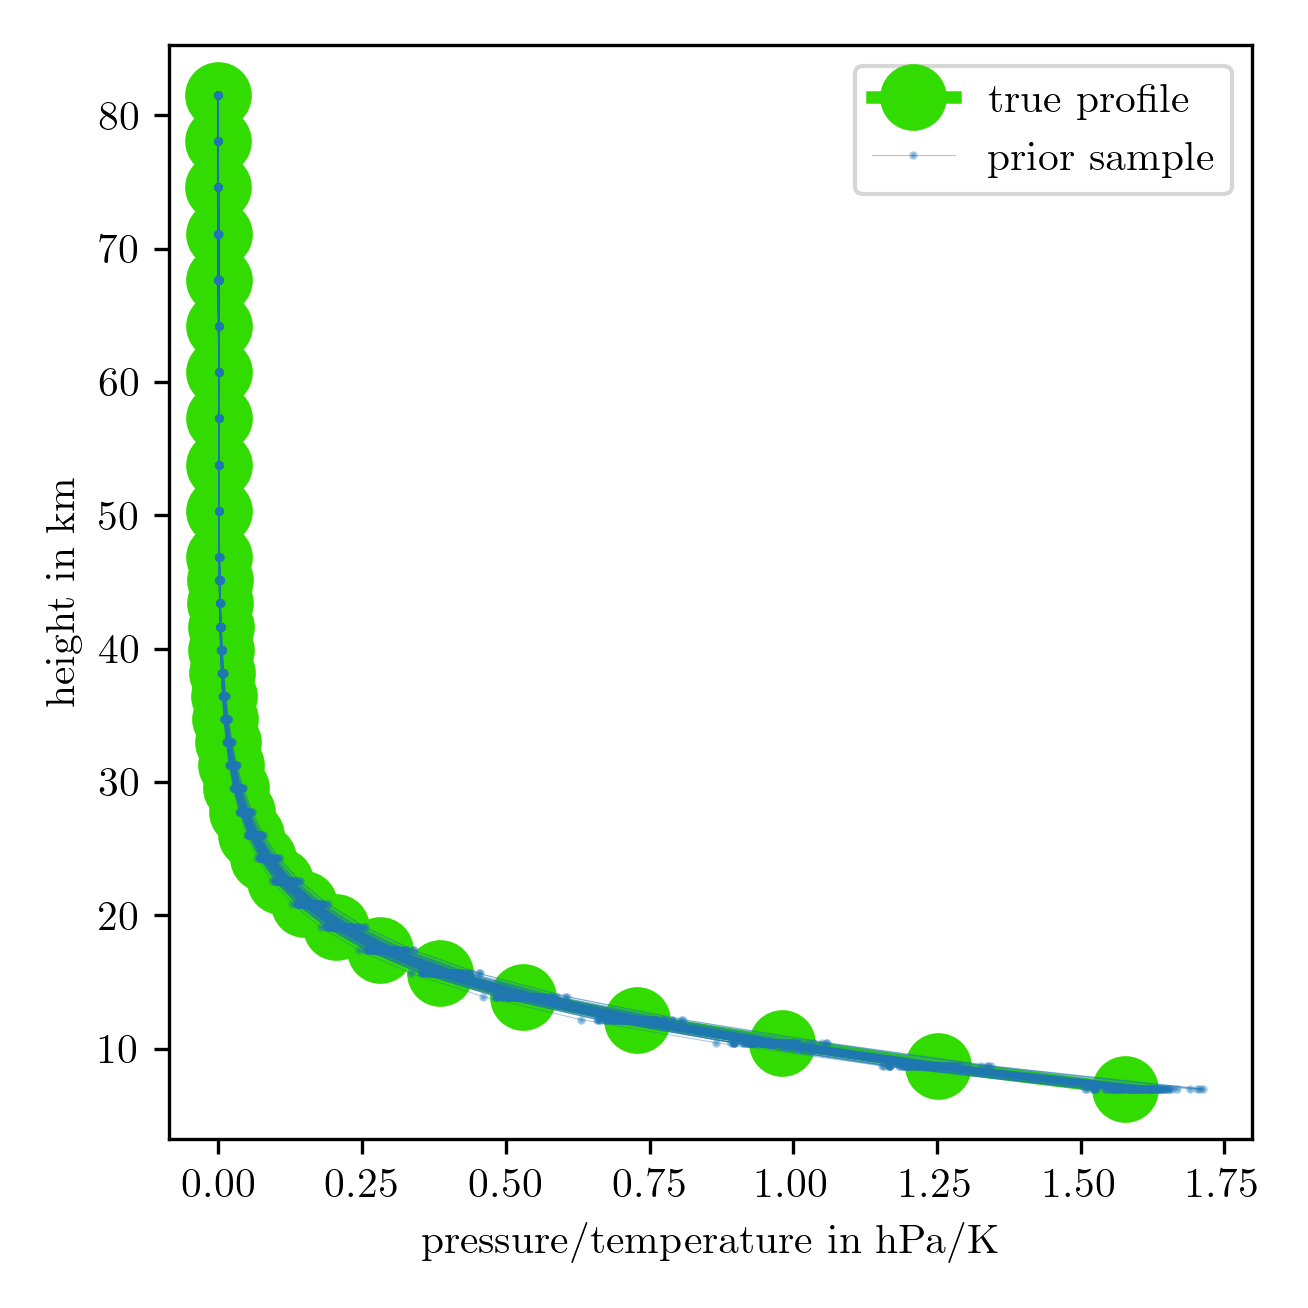
\includegraphics{PriorTempOverPostMeanSigm.png}
	\caption[Prior Samples of $\bm{p}/\bm{T}$ according to the respective hyper-prior distribution.]{We draw samples from the hyper-prior distribution of $h_0, b, p_0, h_1, h_2,h_3,h_4,h_5,h_6, a_0, a_1, a_2,a_3,a_4$ and $T_0$ as defined in table \ref{tab:priors} and then calculate $\bm{p}/\bm{T}$ according to the functions in Eq. \ref{eq:pressFunc} and \ref{eq:tempFunc}.}
	\label{fig:PriorPressOverTemp}
\end{figure}


We plot prior samples of the pressure $\bm{p}$ in Fig. \ref{fig:PriorPress}, the temperature $\bm{T}$ in Fig. \ref{fig:PriorTemp} and the ratio $\bm{p}/\bm{T}$ in Fig. \ref{fig:PriorPressOverTemp} against the ground truth profiles.
Additionally, we plot prior samples of $1/\bm{T}$ in Fig. \ref{fig:OverTempPrior}.
Here we already observe that $\bm{p}/\bm{T}$ inherits the structure of the pressure function and hence the data is uninformative about the temperature, and that is one of the reasons why we chose those hyper-prior distributions.

\subsection{Posterior Distribution}

We either use the \texttt{t-walk} algorithm \cite{christen2010general} to draw samples from $\pi(p_0,b,\bm{h_T},\bm{c_T},\bm{a_T} | \bm{y}, \gamma, \bm{x})$ or we utilise a TT approximation on a predefined grid to then use the SIRT method to draw samples from that posterior.


\subsubsection{Marginal Posterior Distribution}



The aim now is to characterise the posterior
\begin{align}
	\begin{split}
		\pi(p_0,b,T_0,\bm{h_T},\bm{a_T} | \bm{y}, \gamma, \bm{x}) \propto  \exp\Bigl\{ & -\frac{\gamma}{2} \left\Vert \bm{y}- \bm{A} \frac{\bm{p}}{\bm{T}}  \right\Vert^2 \\ &+ \ln{\pi(p_0,b,T_0,\bm{h_T},\bm{a_T})  + c \Bigr\}  }
	\end{split} \, ,
	\label{eq:postPT}
\end{align}
using the approximated forward model $\bm{A} \coloneqq \bm{M}\bm{A}_L$, where $\pi(p_0,b,T_0,\bm{h_T},\bm{a_T})$ is normally distributed, see in Sec. \ref{subsec:PressTempSetup} and Tab. \ref{tab:priors}.
Since “conditioning on estimates gives poor predictive densities” \cite{tan2016LecNot}, we condition on an ozone sample $\bm{x} \sim \pi(\bm{x}|\bm{y})$, see Fig. \ref{fig:O3SolplsReg} and a sample $\gamma \sim \pi(\gamma| \bm{y})$ from the marginal posterior, see Fig. \ref{fig:MargPostHistTT}.
Note that we introduce a "normalisation constant" $c$ for the TT approximation, similar to Sec. \ref{subsec:firstMargTT}.
(5000+100) * 500
2550000
The \texttt{t-walk} \cite{christen2010general} algorithm takes $N = 5 \time 10^6$ steps with a burn-in period of $N_{burn-in} = 100 \times 2500 $, since we expect a maximal IATC, through some pre-analysis, of around 2500, see Tab. \ref{tab:priors}, to generate around $1000$ independent samples from the posterior.
We initialise the \texttt{t-walk} at the hyper-prior mean values and run the t-walk on the negative log of $\pi(p_0,b,T_0,\bm{h_T},\bm{a_T} | \bm{y}, \gamma, \bm{x}) $ (with $c=0$) for $750000$ steps,
This takes around $5$ mins using the \texttt{t-walk} implementation in Python \cite{christentwalkaccess}.
Through some pre-analysis we define hyper-parameters boundaries, which also define the grid bounds for the TT-approximation, see Tab. \ref{tab:priors}.
We plot the resulting histograms in Fig. \ref{fig:PostHistTT0} to \ref{fig:PostHistTT4}.
Additionally, we plot the trace of the samples in Fig. \ref{fig:TraceTwalk}.

\subsubsection{TT-approximation}
To approximate the square root of posterior $\sqrt{\pi(p_0,b,T_0,\bm{h_T},\bm{a_T} | \bm{y}, \gamma, \bm{x})}$ we run the  \texttt{tt.cross.rectcross.rect\_cross.cross} function from the \texttt{ttpy} python package \cite{Oseledets2018ttpy} with constant ranks, which may differ in between each other.
We adjust the constant $c$ for $\pi(p_0,b,T_0,\bm{h_T},\bm{a_T} | \bm{y}, \gamma, \bm{x})$ in Eq. \ref{eq:postPT} to the upper numerical limit of the computer, so that we avoid underflow as much as possible.
More specifically, the upper numerical computer precision is roughly $e^(2*350) approx \infty$, so we evaluate the  $\sqrt{\pi(p_0,b,T_0,\bm{h_T},\bm{a_T} | \bm{y}, \gamma, \bm{x})}$ on 10000 randomly choose grid points and conservatively set the constant so that the maximum values of those grid point is $\approx 325$.
This may change depending on the ozone and $\gamma$ sample we condition on, for the data set we choose to the pre-ananlysis this constant is $328$. 
Then we can compute the marginal as in Sec. \ref{sec:tensortrain}, where we set $\xi = 1 / \uplambda (\mathcal{X})$ and $\uplambda(x) = 1$ so that for Cartesian basis $\bm{M}_k = \text{diag}(\uplambda_k(\mathcal{X}_k))$.
We initialise the \texttt{cross}  with a random tensor and we run 5 sweeps it takes roughly $3$ to $4$min.

\begin{figure}[h]% will be the left-side figure
	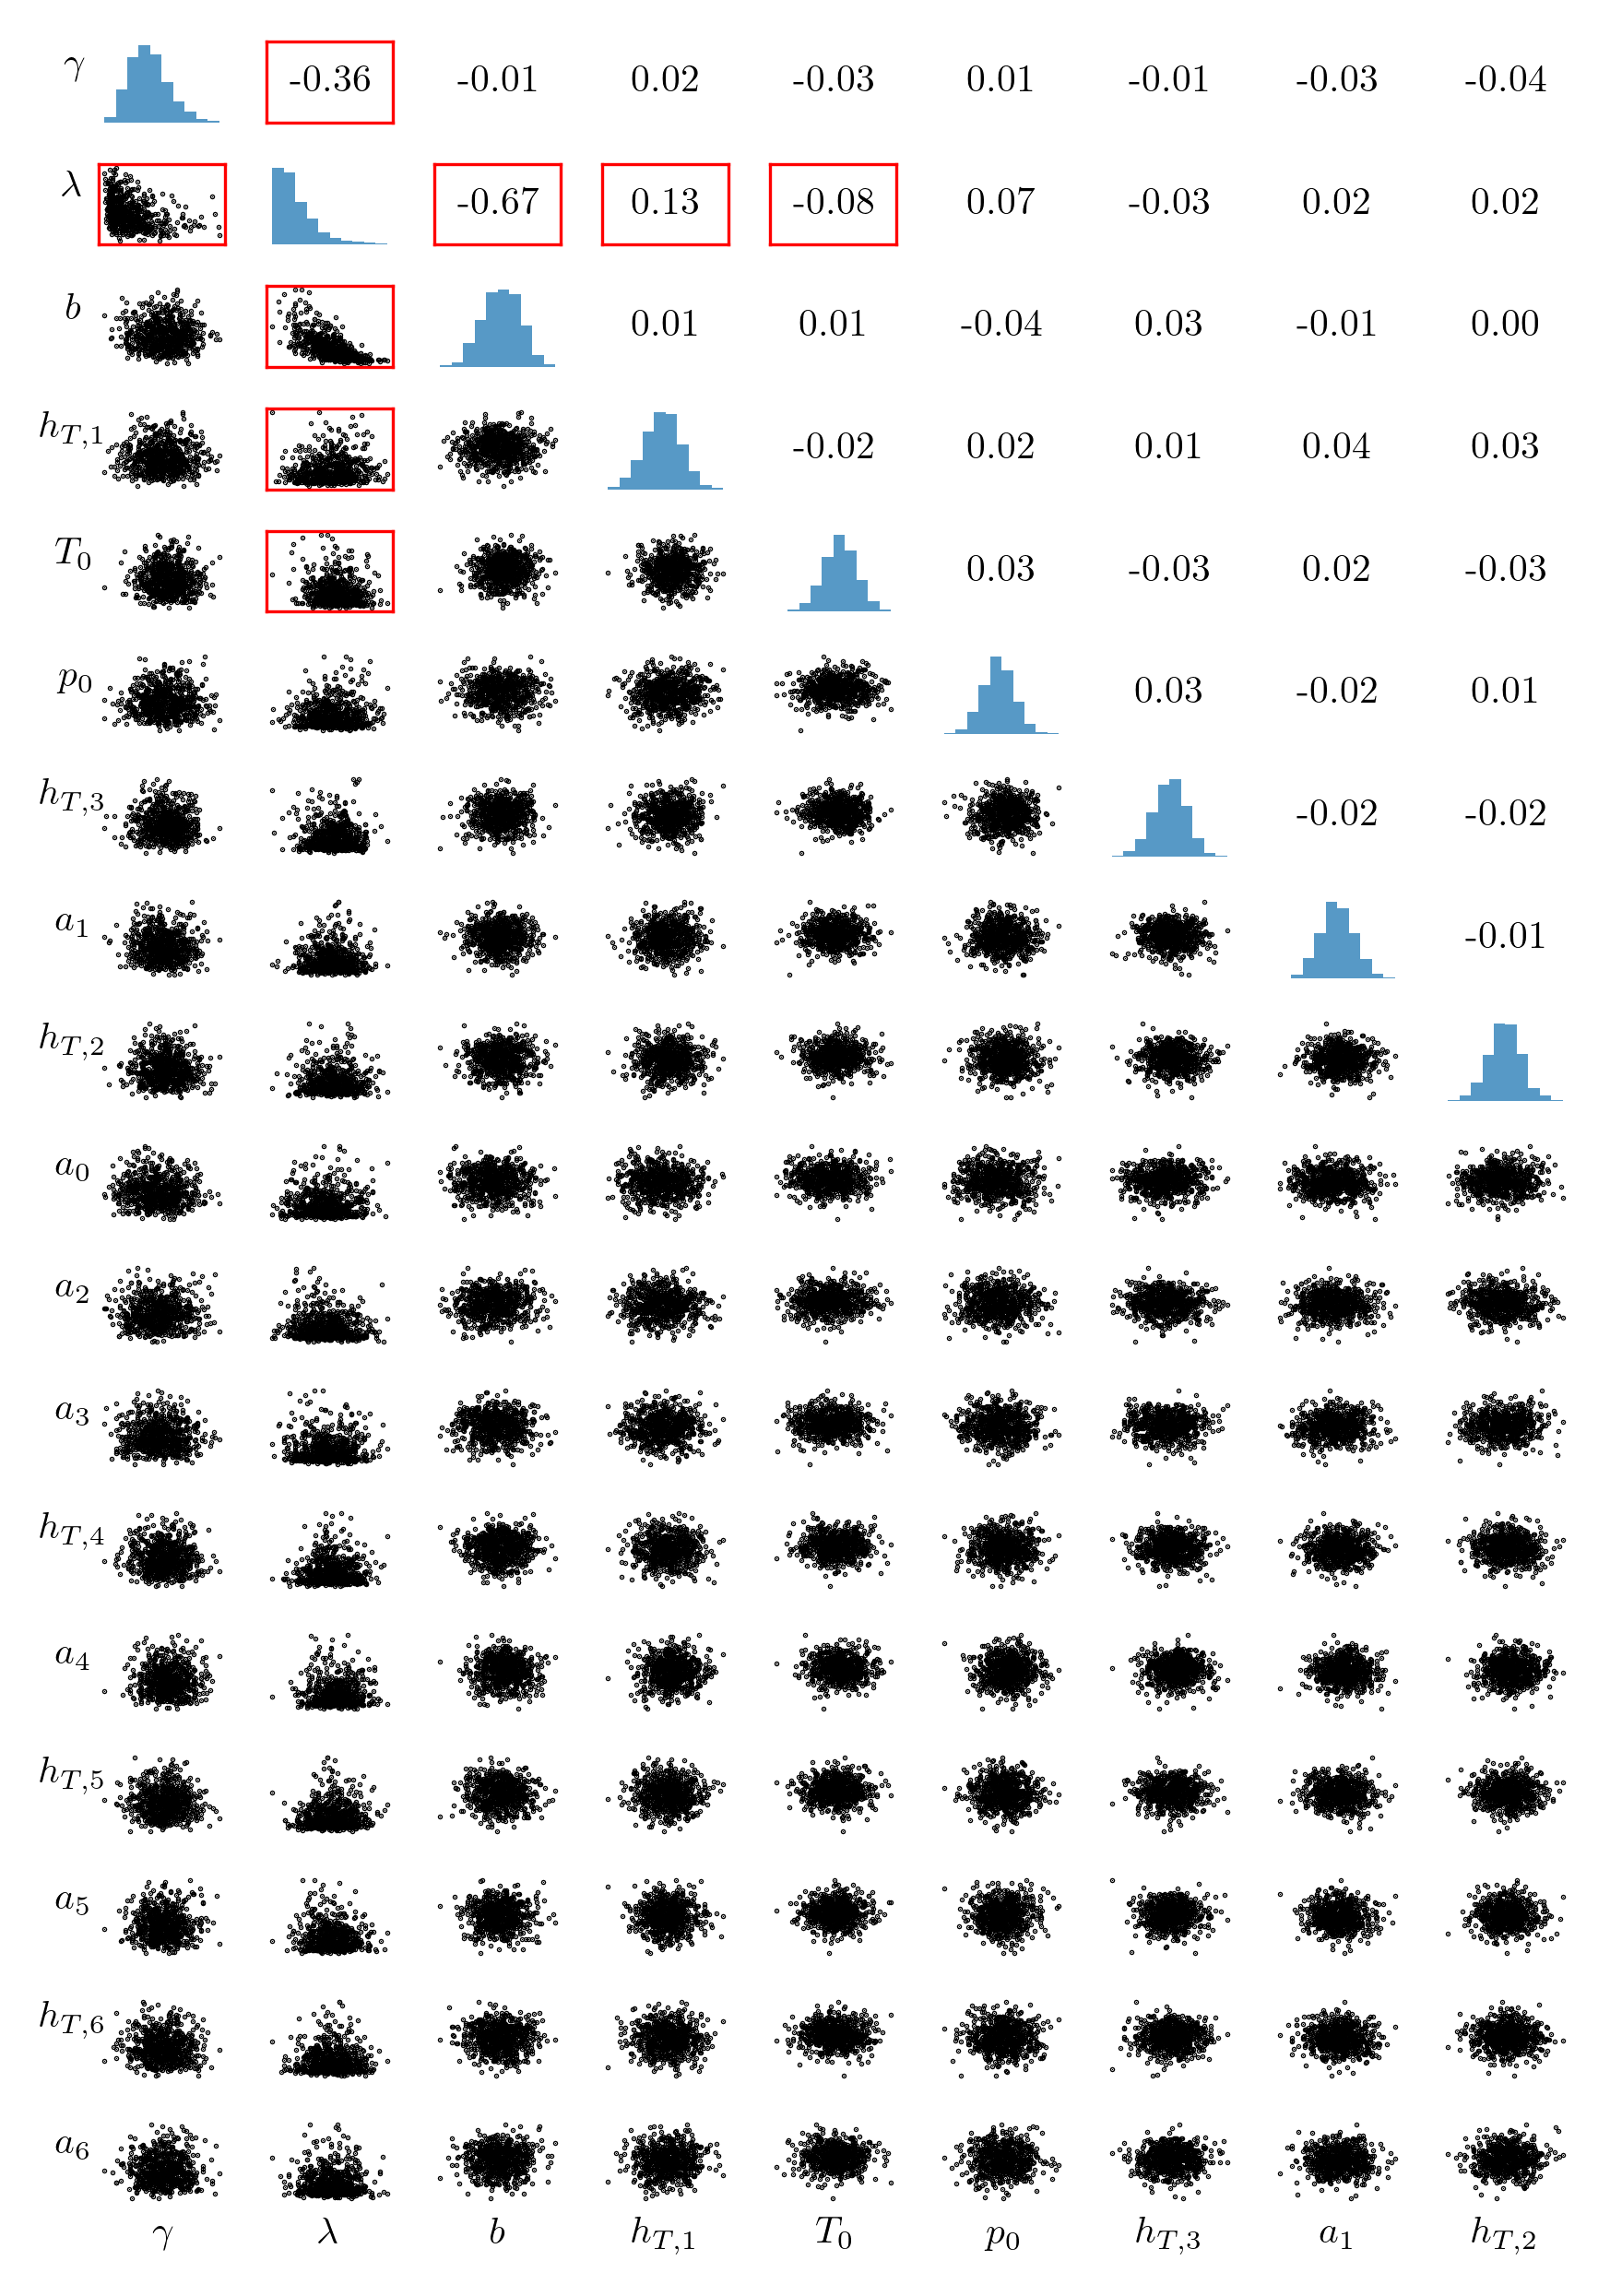
\includegraphics[]{CorrPlot.png}
	\caption[Correlation plot of samples from TT-approximation]{Scatter plot of samples from TT-approximation of $\sqrt{\pi(p_0,b,T_0,\bm{h_T},\bm{a_T} | \bm{y}, \gamma, \bm{x})}$ via SIRT scheme. We plot the Pearson correlation coefficient ranging from $-1$ to $1$ for each hyper-parameter pair.}
	\label{fig:CorrPlot}
\end{figure}
\begin{figure}% will be the right-side figure
	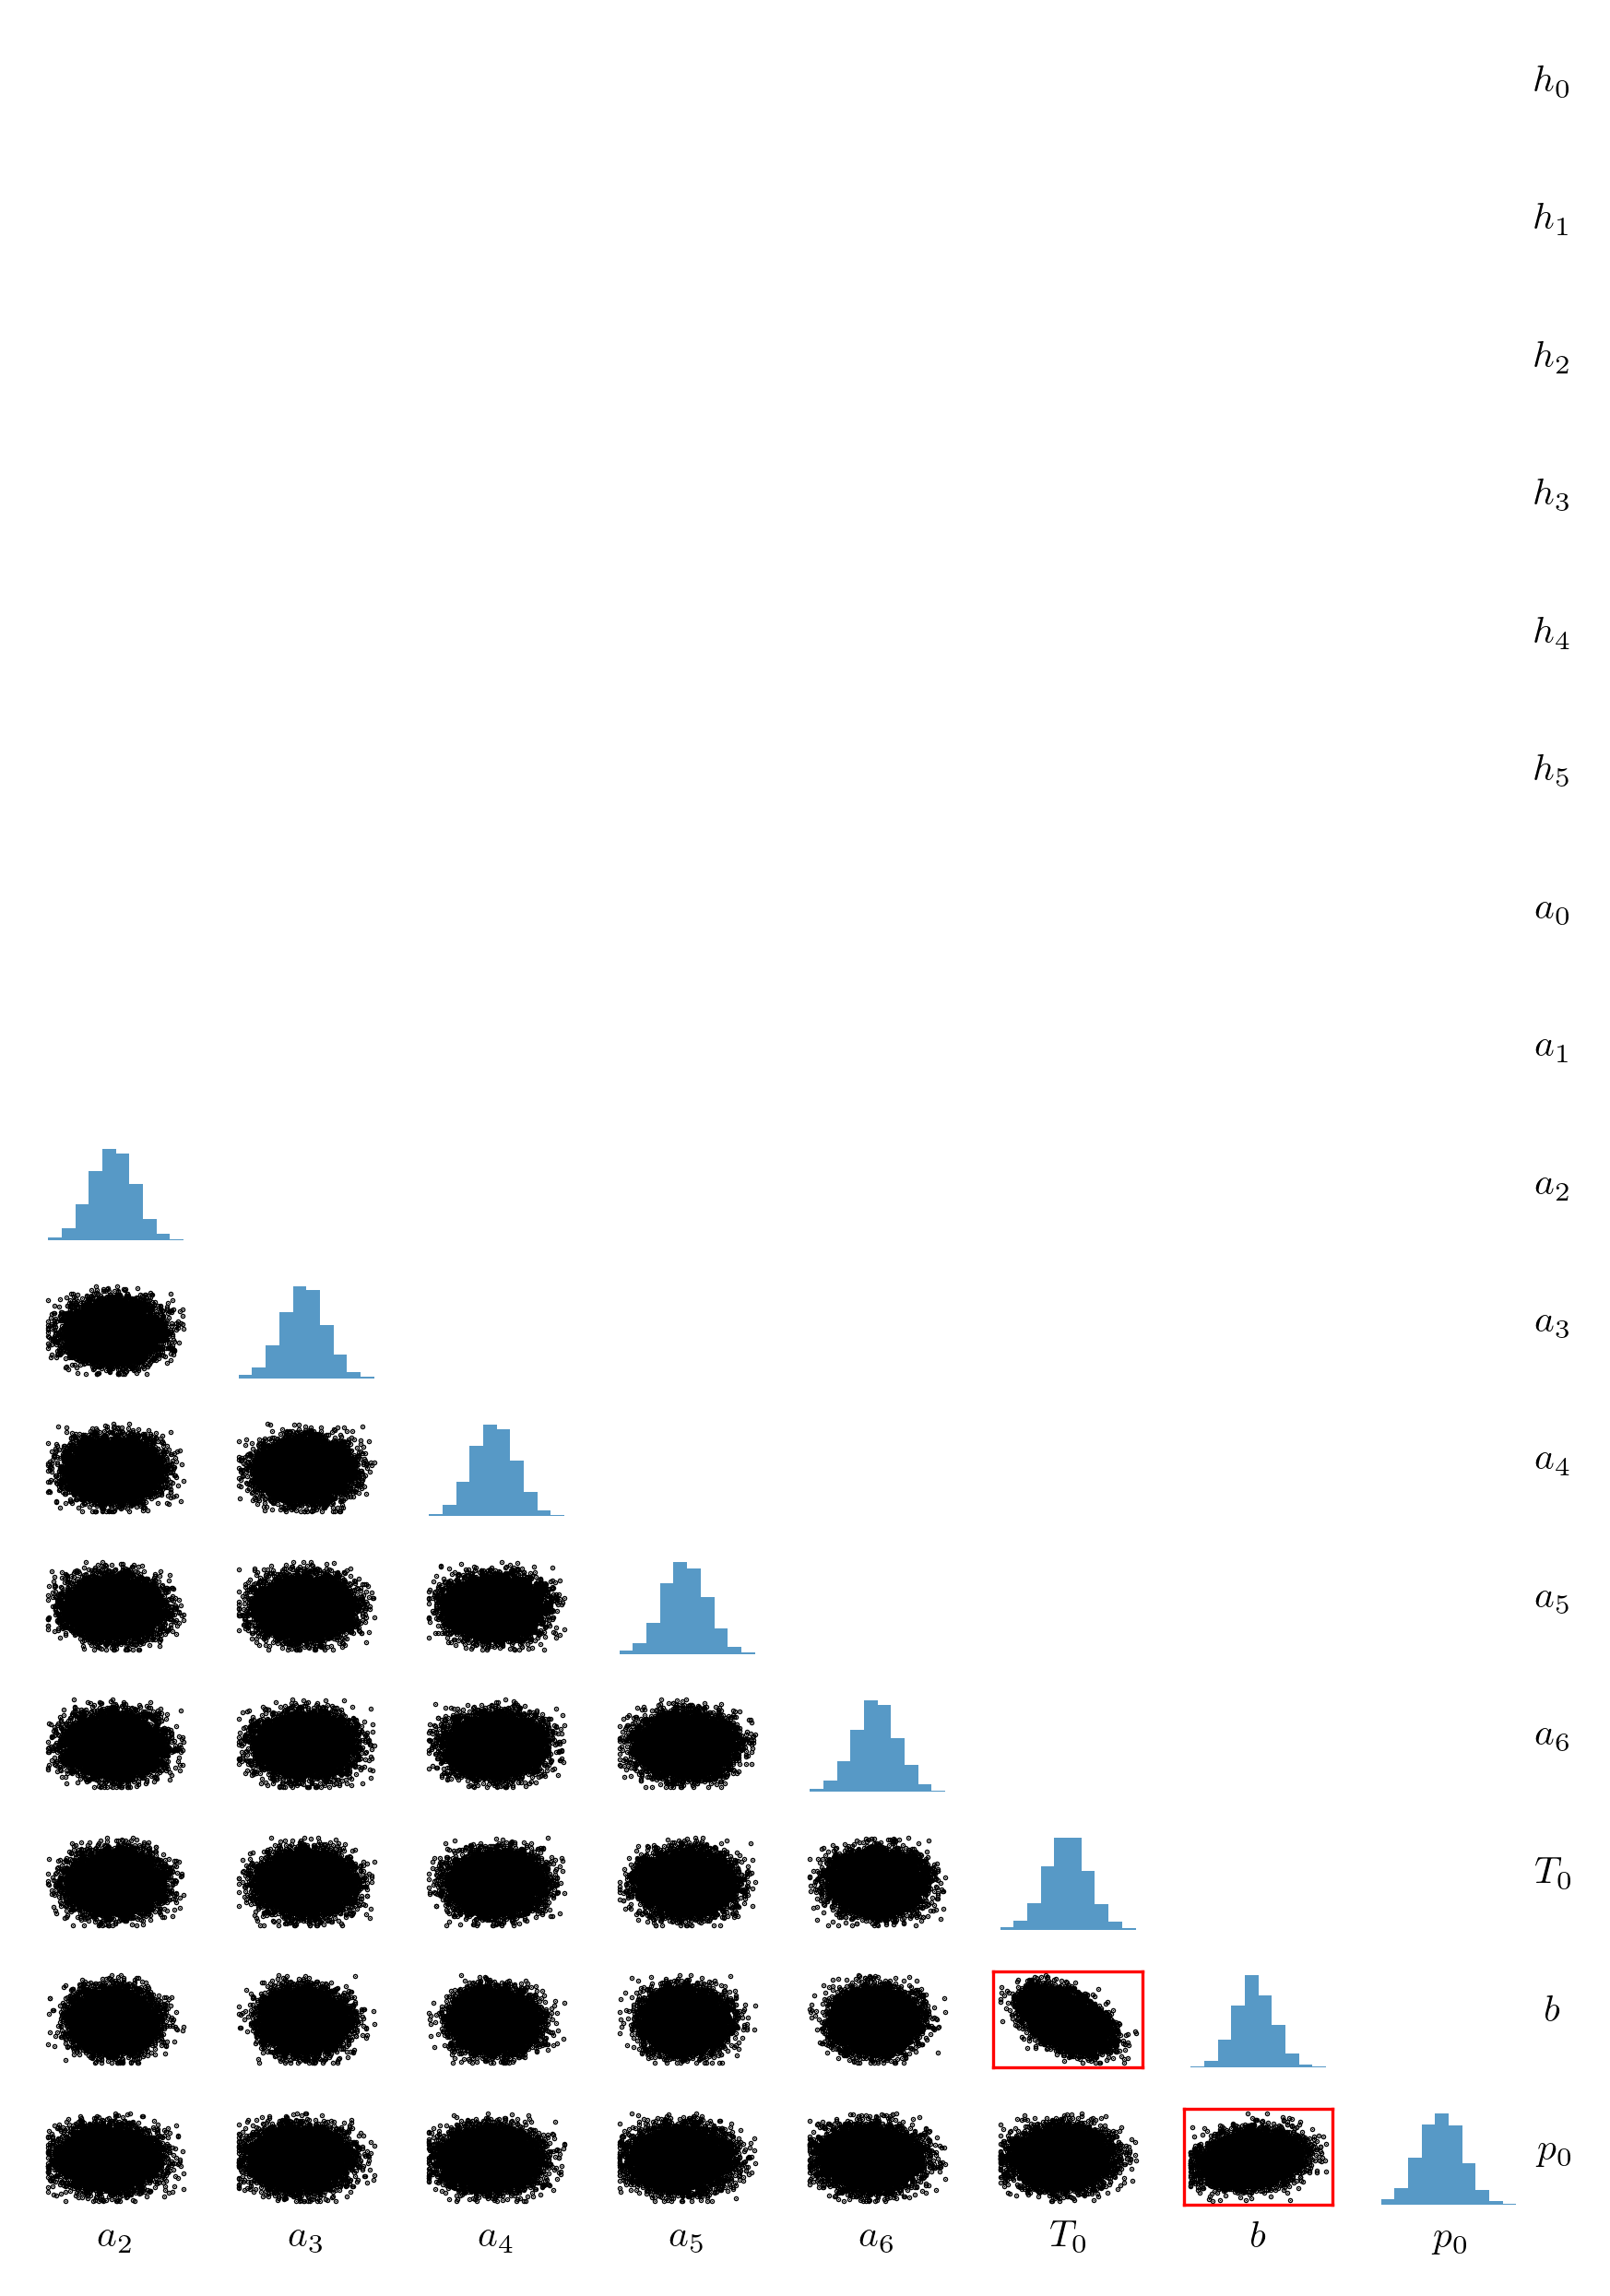
\includegraphics[]{2ndCorrPlot.png}
	\caption*{Correlation plot of samples from TT-approximation of $\sqrt{\pi(p_0,b,T_0,\bm{h_T},\bm{a_T} | \bm{y}, \gamma, \bm{x})}$ via SIRT scheme.}
\end{figure}
\cleardoublepage
The First thing we do is to arrange the order of parameters according to their correlation structure.
This means we have highly correlated parameter pairs next each other, so that their TT-cores are direct neighbours and linked through their shared rank.
See Fig.\ref{fig:CorrPlot}, where we scatter plot the samples from the TT-approximation od $\sqrt{\pi(p_0,b,T_0,\bm{h_T},\bm{a_T} | \bm{y}, \gamma, \bm{x})}$ via SIRT scheme.
Additionally, we calculate and plot the Pearson correlation, where a coefficient close to zero corresponds to low correlational and a coefficient close to $1$ or $-1$ corresponds to high correlation.
We observe that the hyper-parameters describing pressure and the hyper-parameters describing the temperature function in low altitudes are far more correlated than hyper-parameters corresponding to higher altitudes, see also IATC in Tab. \ref{tab:priors}.
We try to arrange the parameters so that the correlation coefficient are increasing towards the diagonal, we do this iteratively by exploratory analysis.
Next we aim to find the optimal rank and grid size to approximate $\sqrt{\pi(p_0,b,T_0,\bm{h_T},\bm{a_T} | \bm{y}, \gamma, \bm{x})}$, so that the number of function evaluation are as low as possible but not 


Next, we choose a relatively large number of grid points and calculate different error measures for deceasing number of ranks to find the optimal number of ranks.
We set the number of grid point to $n = 150$ and calculate the 1-Wasserstein distance, see Sec. \ref{subsec:wasser}, between the samples from the t-walk and samples from the TT-approximation using the SIRT scheme, weighted according to their posterior distribution values.  
To calculate the 1-Wasserstein distance, as in Eq. \ref{eq:applWasser}, we use the \texttt{SamplesLoss("sinkhorn", p=1, blur=0.05, scaling=0.8)} function with default settings from the python package \texttt{geomloss} \cite{Wassersteinaccess}.
This provides the unbiased Sinkhorn divergence which converges towards the Wasserstein distance and can be understood as the generalised Quicksort algorithm \cite{feydy2020OT}.
Here, p = 1 defines the distance measure $\lVert \bm{x} -\tilde{\bm{x}} \rVert_{L^2}$, the blur parameter can be understood as an entropic penalty and the  scaling parameter specifies the trade-off between speed (scaling < .4) and accuracy (scaling > .9) \cite{Wassersteinaccess}.
Additionally we use the marginal functions to calculate the mean of each hyper-parameter and then the relative RMS error over all of those means, as well as the relative RMS error of the TT-approximation, evaluated at the samples from the SIRT scheme.

\begin{figure}[ht!]% will be the left-side figure
	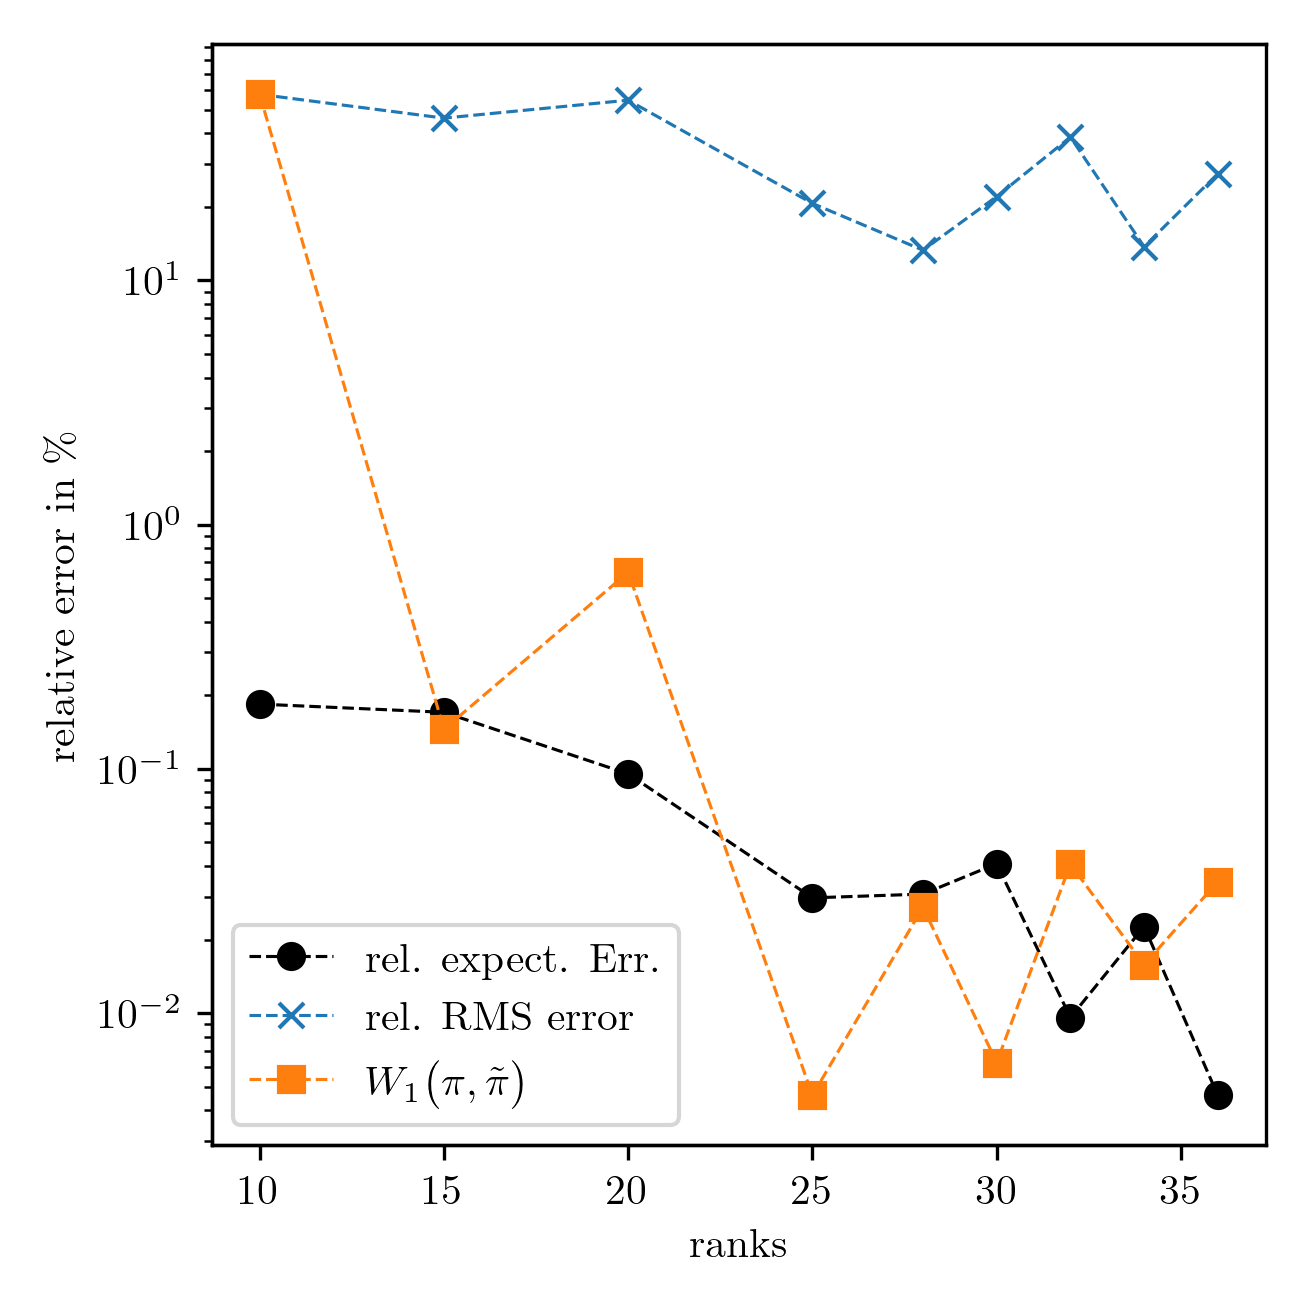
\includegraphics[]{findRank.png}
	\caption[Find Ranks]{}
	\label{fig:FindRanks}
\end{figure}
In Fig. \ref{fig:FindRanks}, we see that the Wasserstein distance decreases rapidly as well as the rel. error of the means.
The RMS error is constant around $10\%$, and does not decrease much after a rank of $r = 30$.
Since we can also plot the marginal and compare to samples from the \texttt{t-walk} we can easily observe non smooth solutions for which the wasserstein distance and the rel. error of means is low.
This indicates that we do not necessarily need a good approximation, with an MH correction step and integratin we find that this does not matter too much.
To be on the safe side we choose a rank of $r = 40$ and then decrease the grid-size to find the minimum grid size which still gives good solutions.

Given the choosen rank we want to decrease the gridsize, to $r =n$.
And firthrte fot rcomputaionlas efficeny we decrease rank wjhere the corrlatino structire is low.
\begin{figure}[h]% will be the left-side figure
	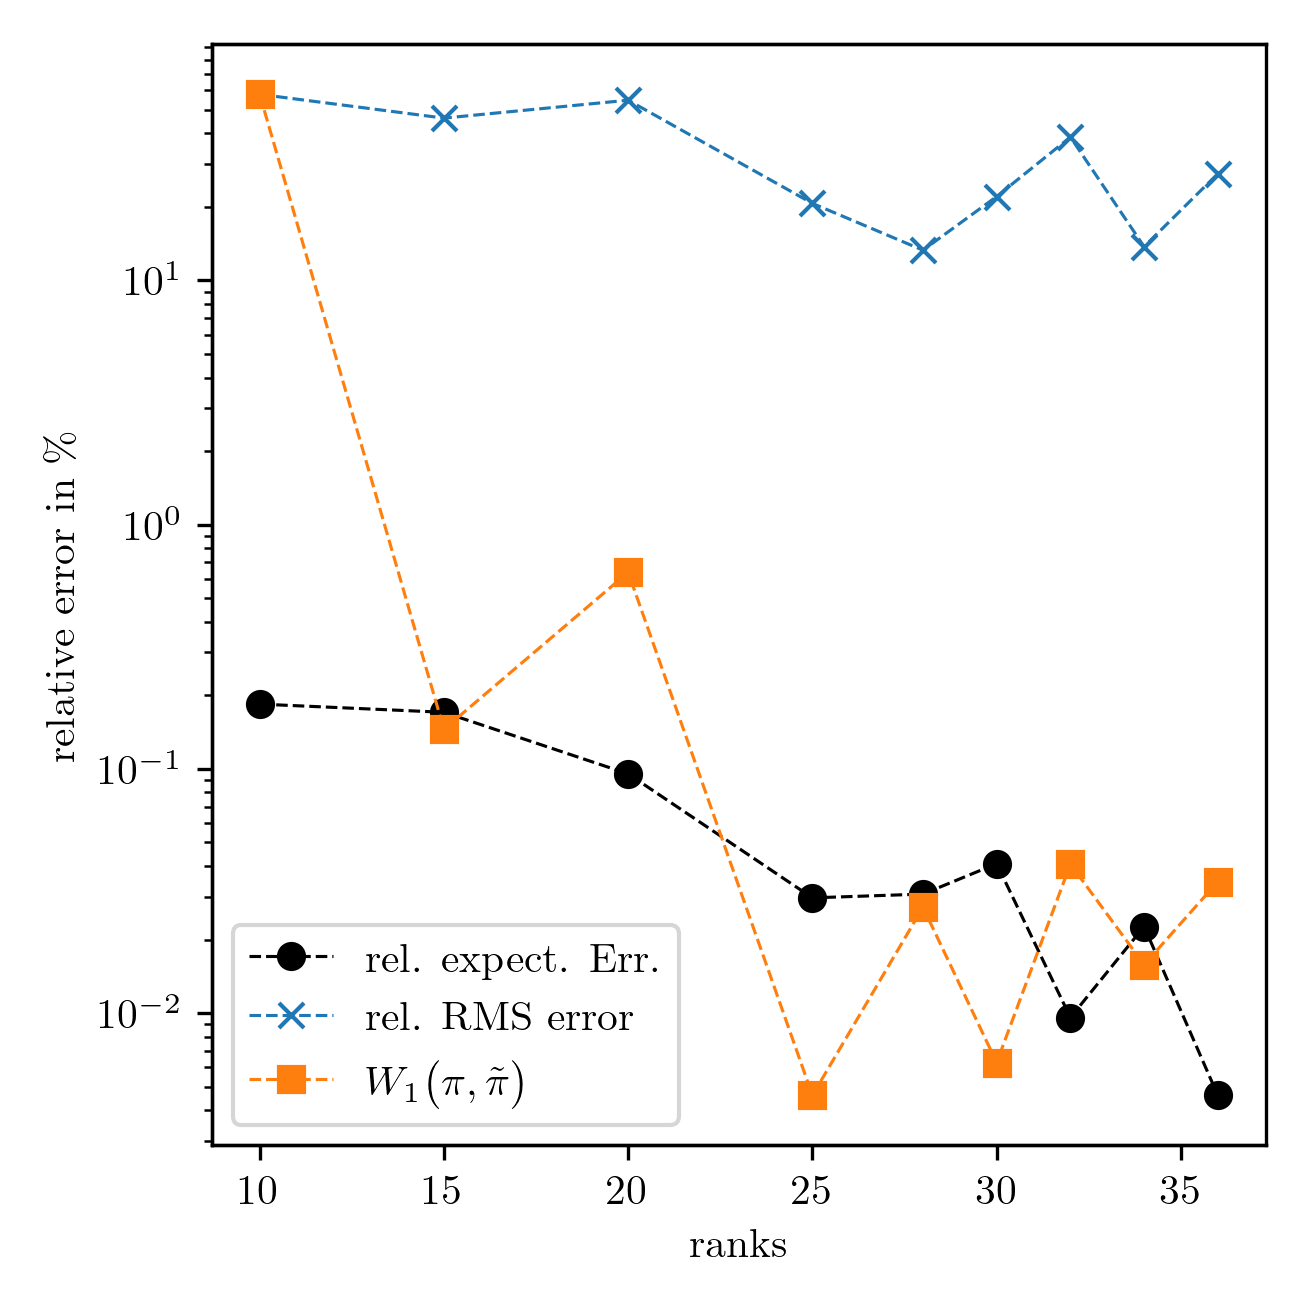
\includegraphics[]{findRank.png}
	\caption[Find Grid]{}
	\label{fig:FindGrid}
\end{figure}
\clearpage

We push firther and defin ranks $r = [ 1, 35,  35, 35, 35, 20, 10, 10, 5, 3, 2, 2, 2, 2, 2, 2, 1]$
Which reduces compuatalle time and number of function evaluation drastcailly.
We compare that to our results of the T sampler and TT and see that they are prettry muich the dame
We report an rms error and a realtive in error in experations as 
Note that we can reduce the number of sweeps siginifantlc y of we us a pre tensor soutionm isnteda of arandom 
then we need one sweep and are in bussinins.

\begin{figure}[ht!]
	\centering
	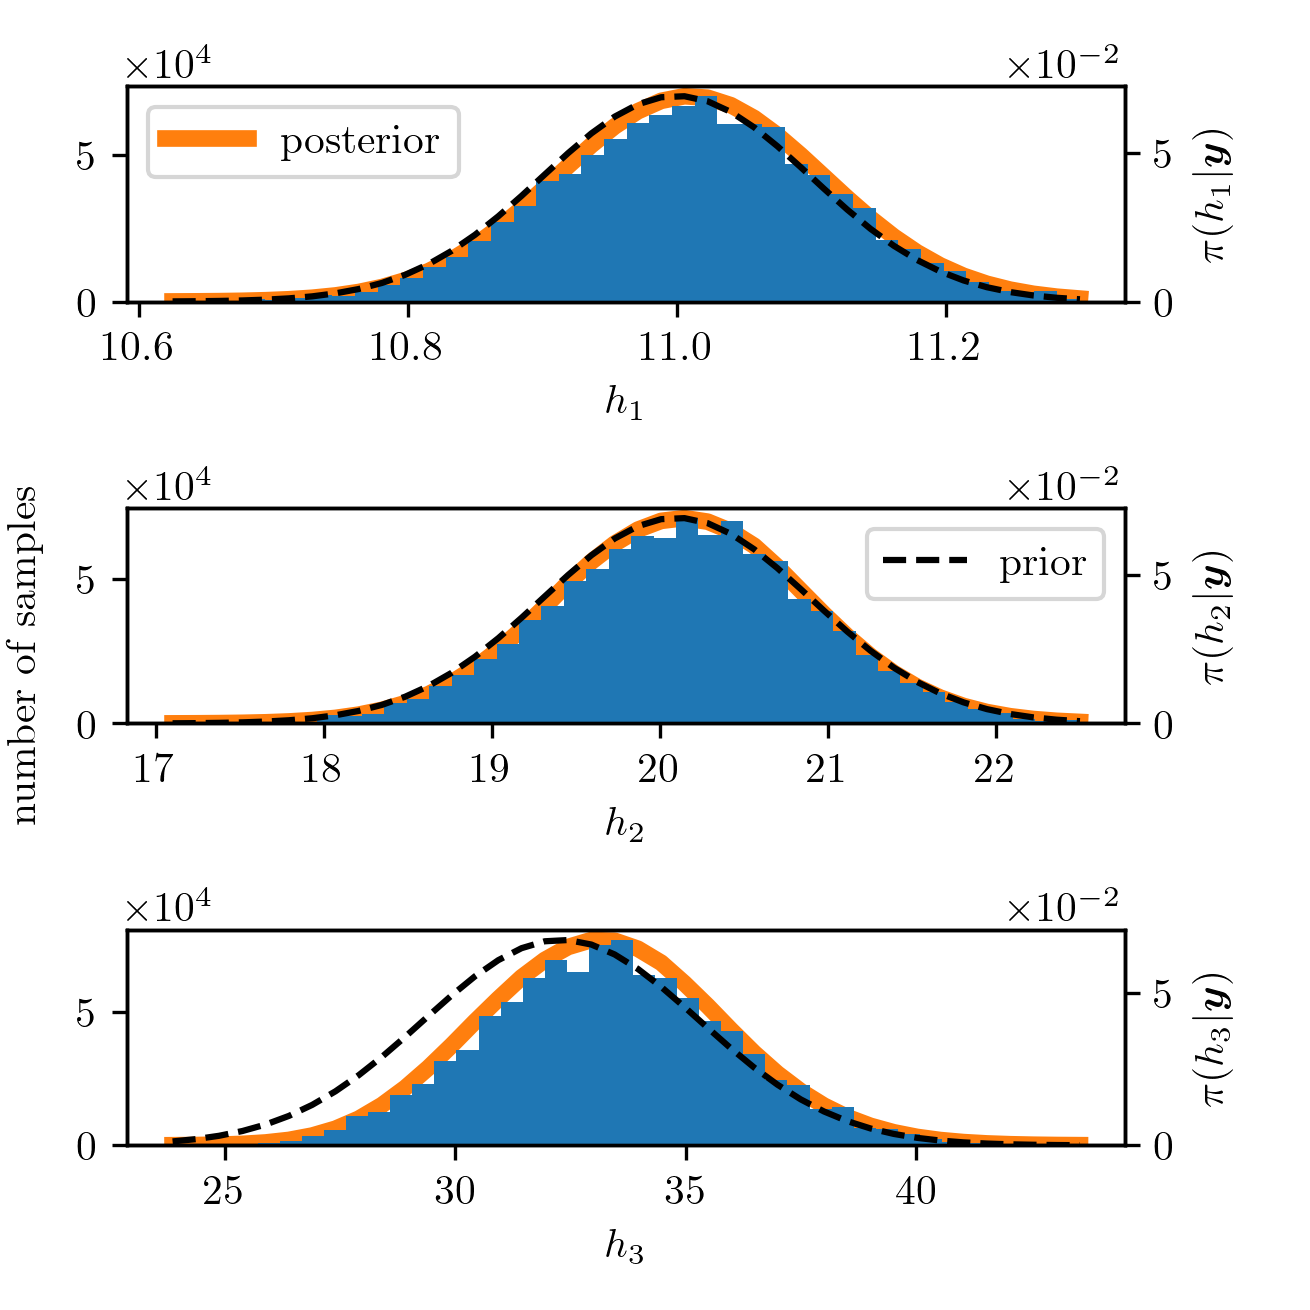
\includegraphics{PHdPTPost0.png}
	\caption[Histograms and TT approximation of posterior distribution as well as hyper-prior distribution.]{We plot the TT approximation of marginal posterior in orange and the samples as a histogram as well as the prior distribution with a dotted line.}
	\label{fig:PostHistTT0}
\end{figure}
\begin{figure}[ht!]
	\centering
	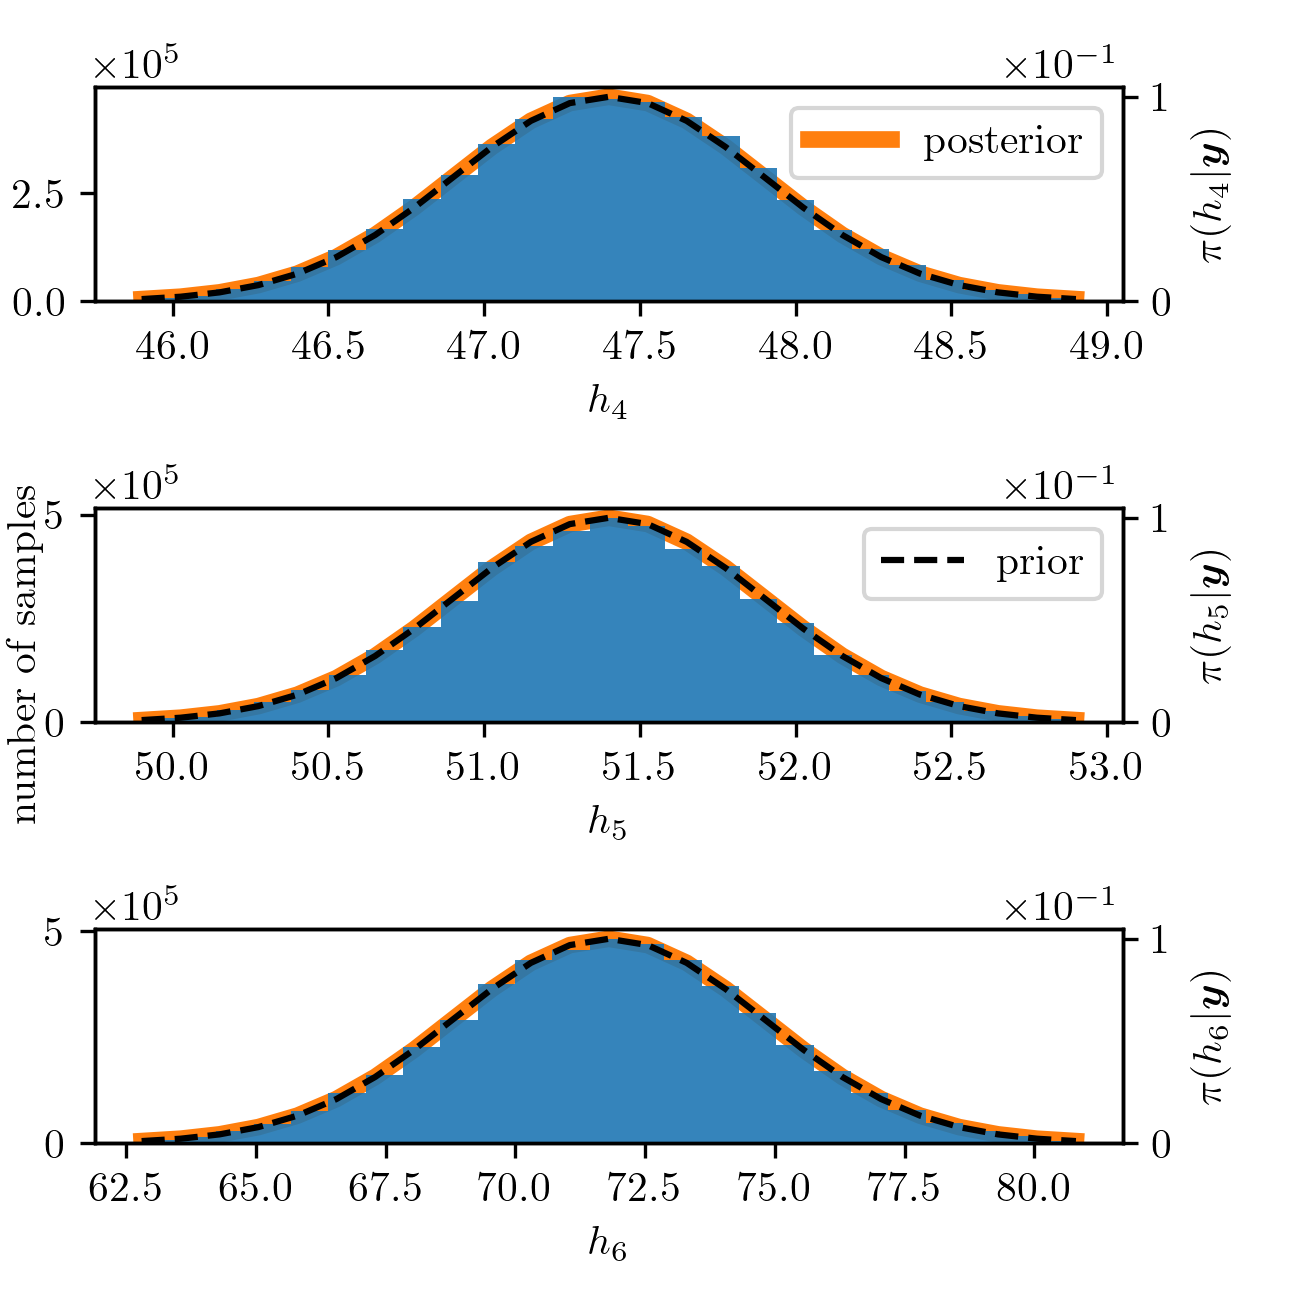
\includegraphics{PHdPTPost1.png}
	\caption[Histograms and TT approximation of posterior distribution as well as hyper-prior distribution.]{We plot the TT approximation of marginal posterior in orange and the samples as a histogram as well as the prior distribution with a dotted line.}
	\label{fig:PostHistTT1}
\end{figure}
\begin{figure}[ht!]
	\centering
	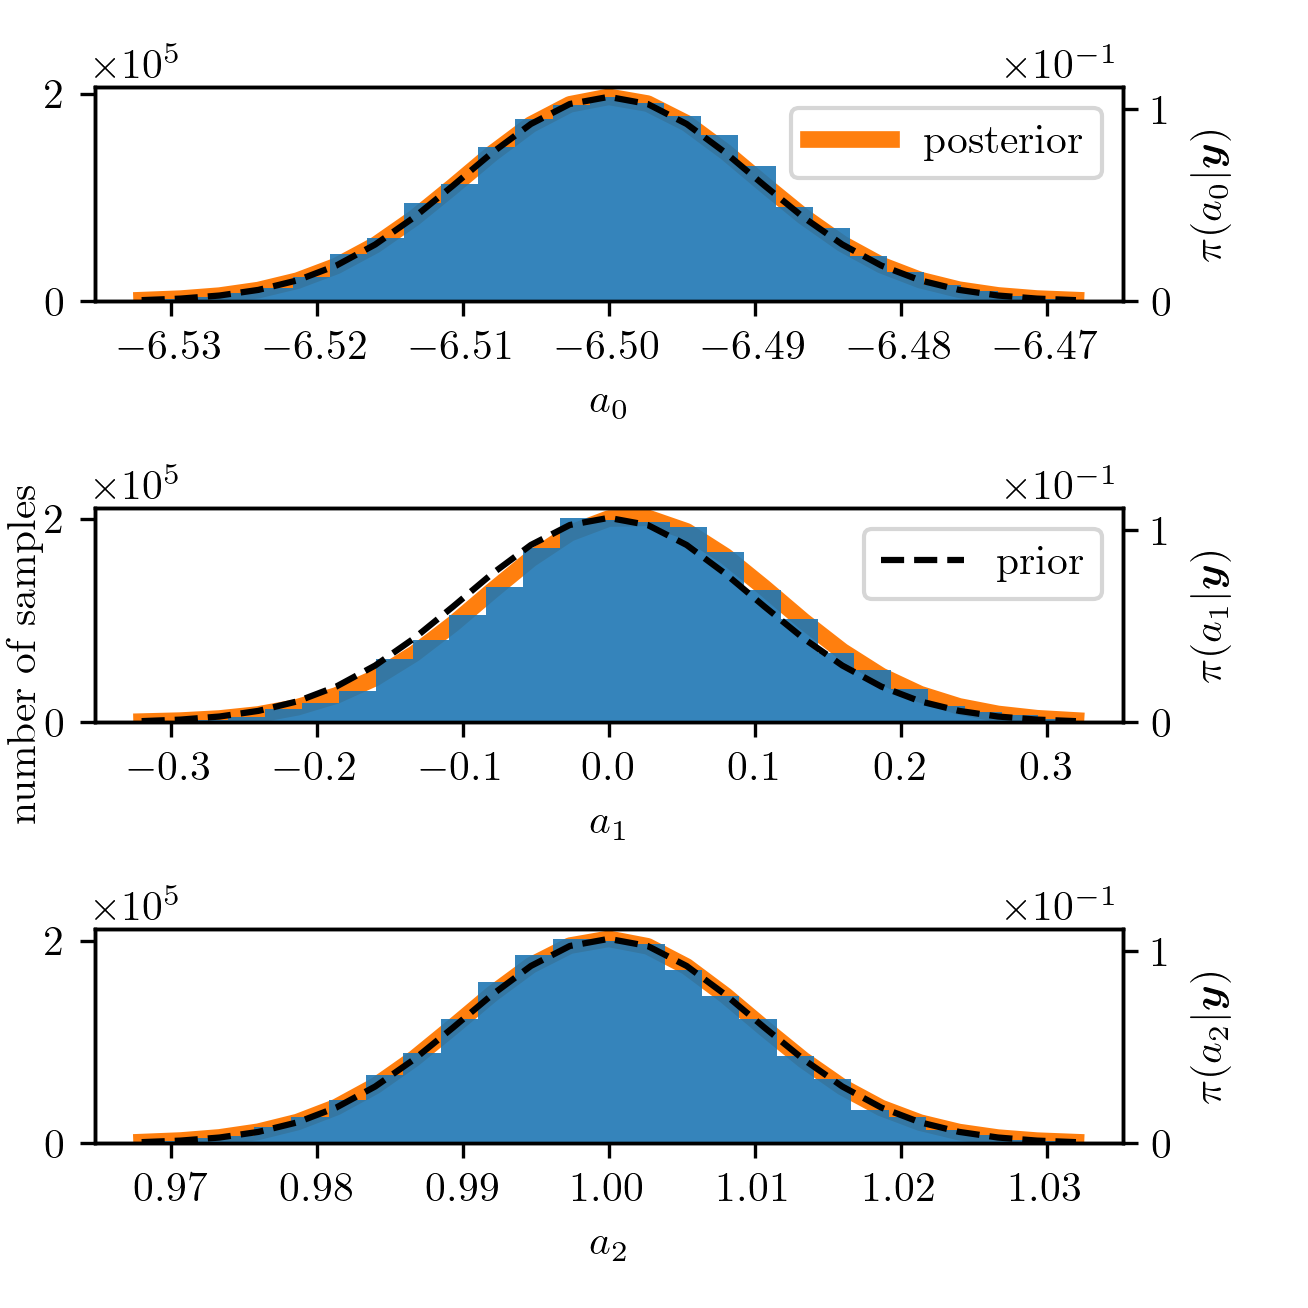
\includegraphics{PHdPTPost2.png}
	\caption[Histograms and TT approximation of posterior distribution as well as hyper-prior distribution.]{We plot the TT approximation of marginal posterior in orange and the samples as a histogram as well as the prior distribution with a dotted line.}
	\label{fig:PostHistTT2}
\end{figure}
\begin{figure}[ht!]
	\centering
	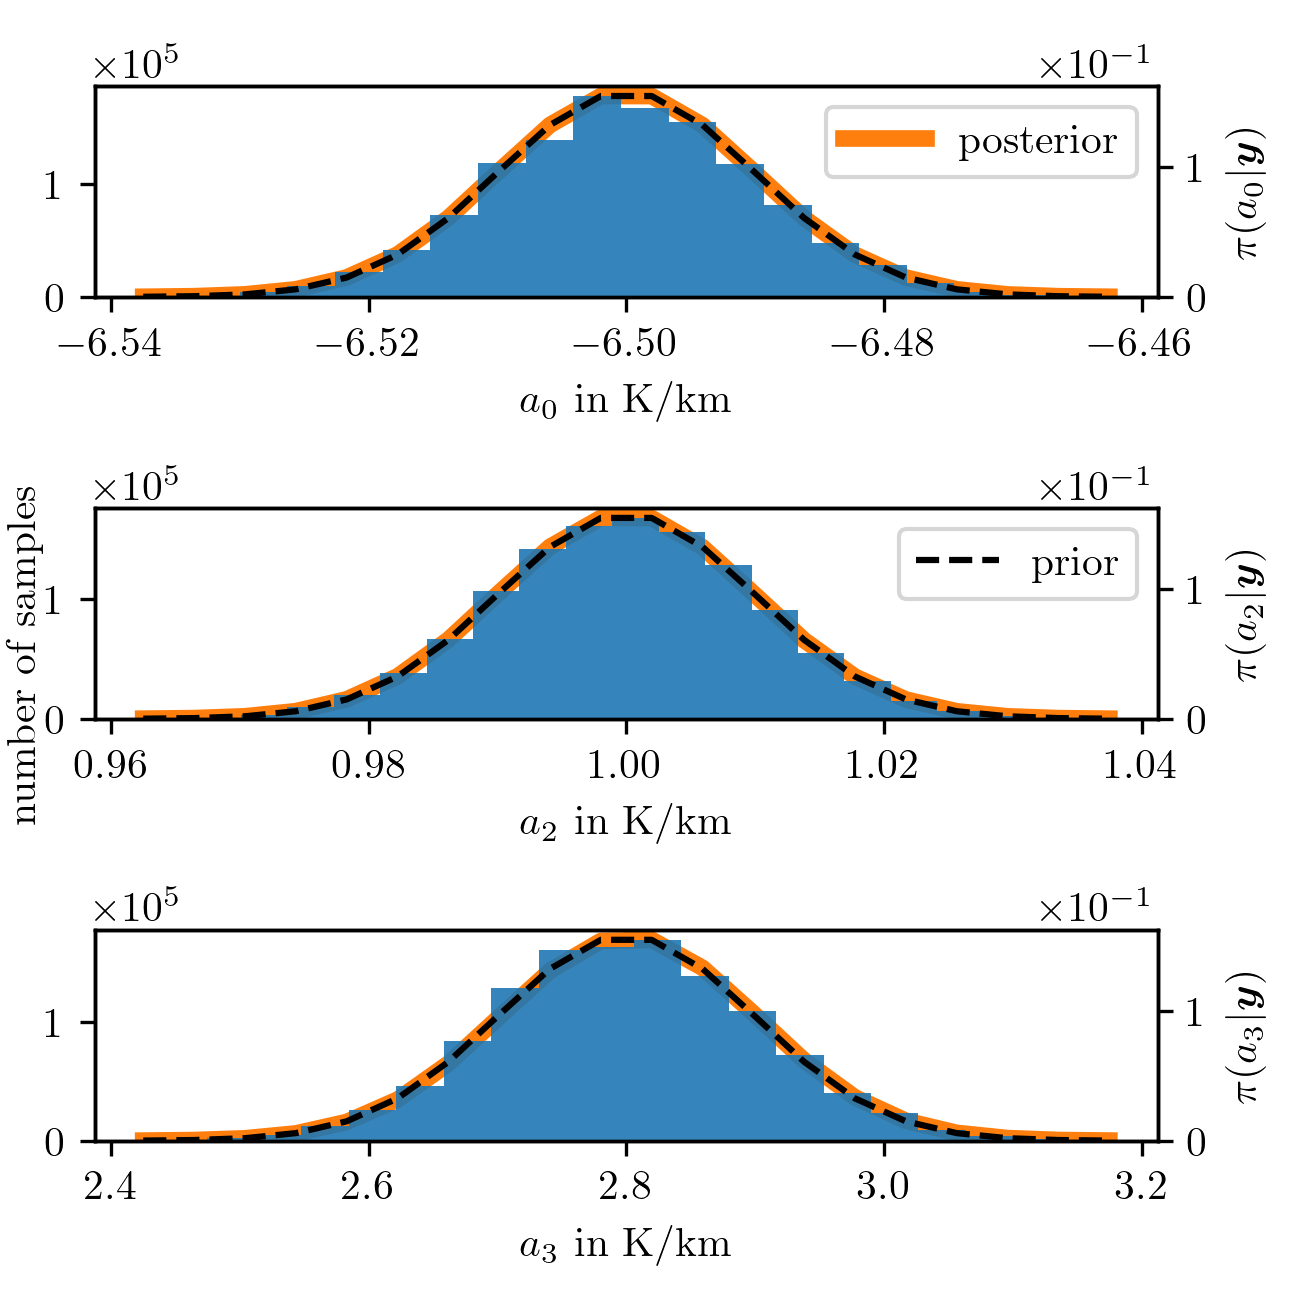
\includegraphics{PHdPTPost3.png}
	\caption[Histograms and TT approximation of posterior distribution as well as hyper-prior distribution.]{We plot the TT approximation of marginal posterior in orange and the samples as a histogram as well as the prior distribution with a dotted line.}
	\label{fig:PostHistTT3}
\end{figure}
\begin{figure}[ht!]
	\centering
	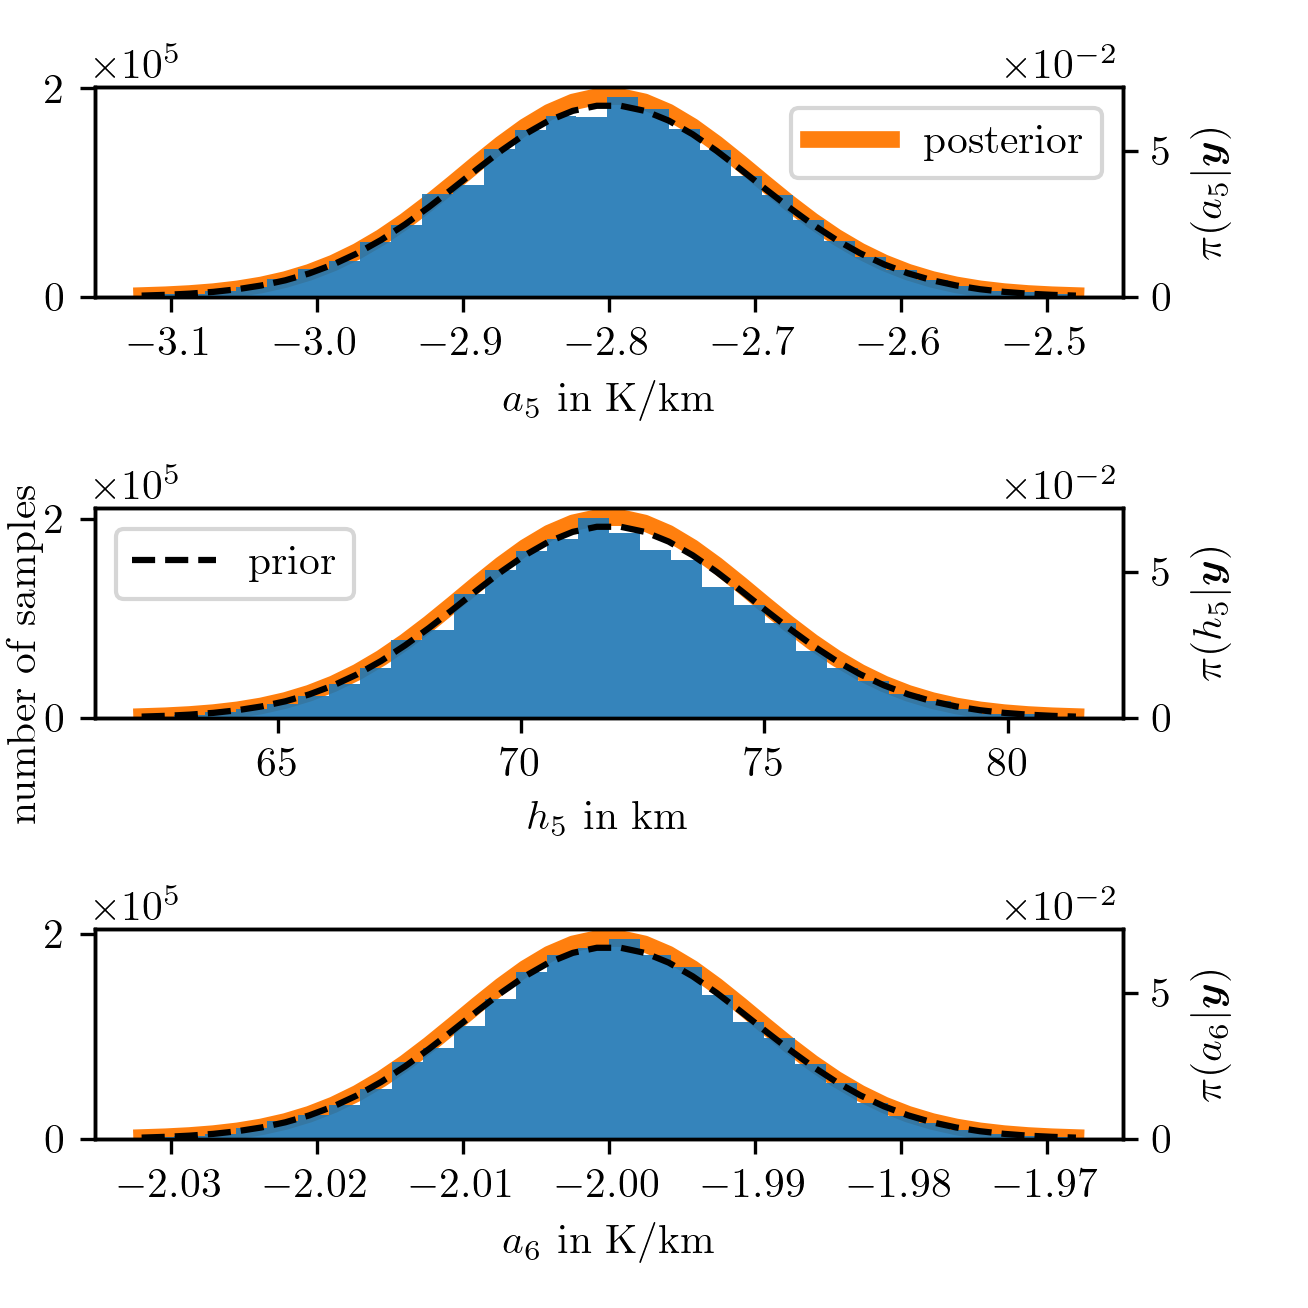
\includegraphics{PHdPTPost4.png}
	\caption[Histograms and TT approximation of posterior distribution as well as hyper-prior distribution.]{We plot the TT approximation of marginal posterior in orange and the samples as a histogram as well as the prior distribution with a dotted line.}
	\label{fig:PostHistTT4}
\end{figure}
\begin{figure}[ht!]
	\centering
	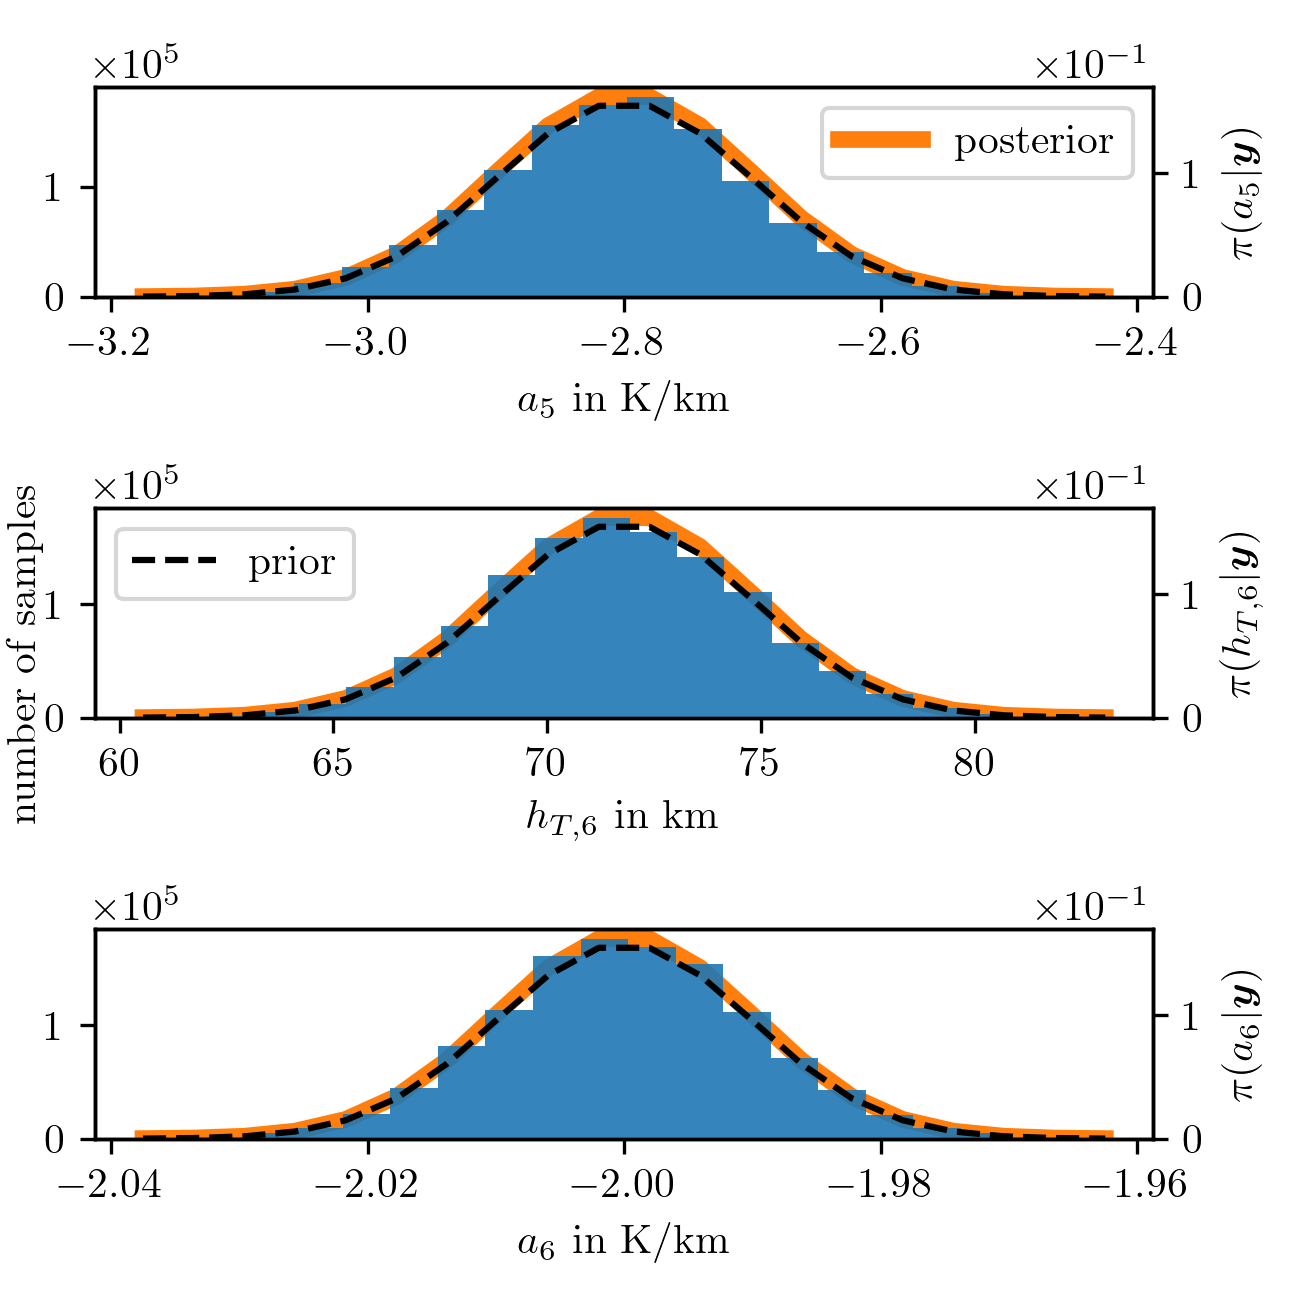
\includegraphics{PHdPTPost5.png}
	\caption[Histograms and TT approximation of posterior distribution as well as hyper-prior distribution.]{We plot the TT approximation of marginal posterior in orange and the samples as a histogram as well as the prior distribution with a dotted line.}
	\label{fig:PostHistTT5}
\end{figure}
\clearpage





\subsubsection{Conditional Posterior Distribution}
To obtain temperature and pressure profiles, we can either take samples from the output of the t-walk or generate random values between 0 and 1 and compare them to the cumulative distribution functions.
We plot the posterior temperature and pressure profiles in Fig. \ref{fig:TempPost} and Fig. \ref{fig:PressPost}.
\begin{figure}[ht!]
	\centering
	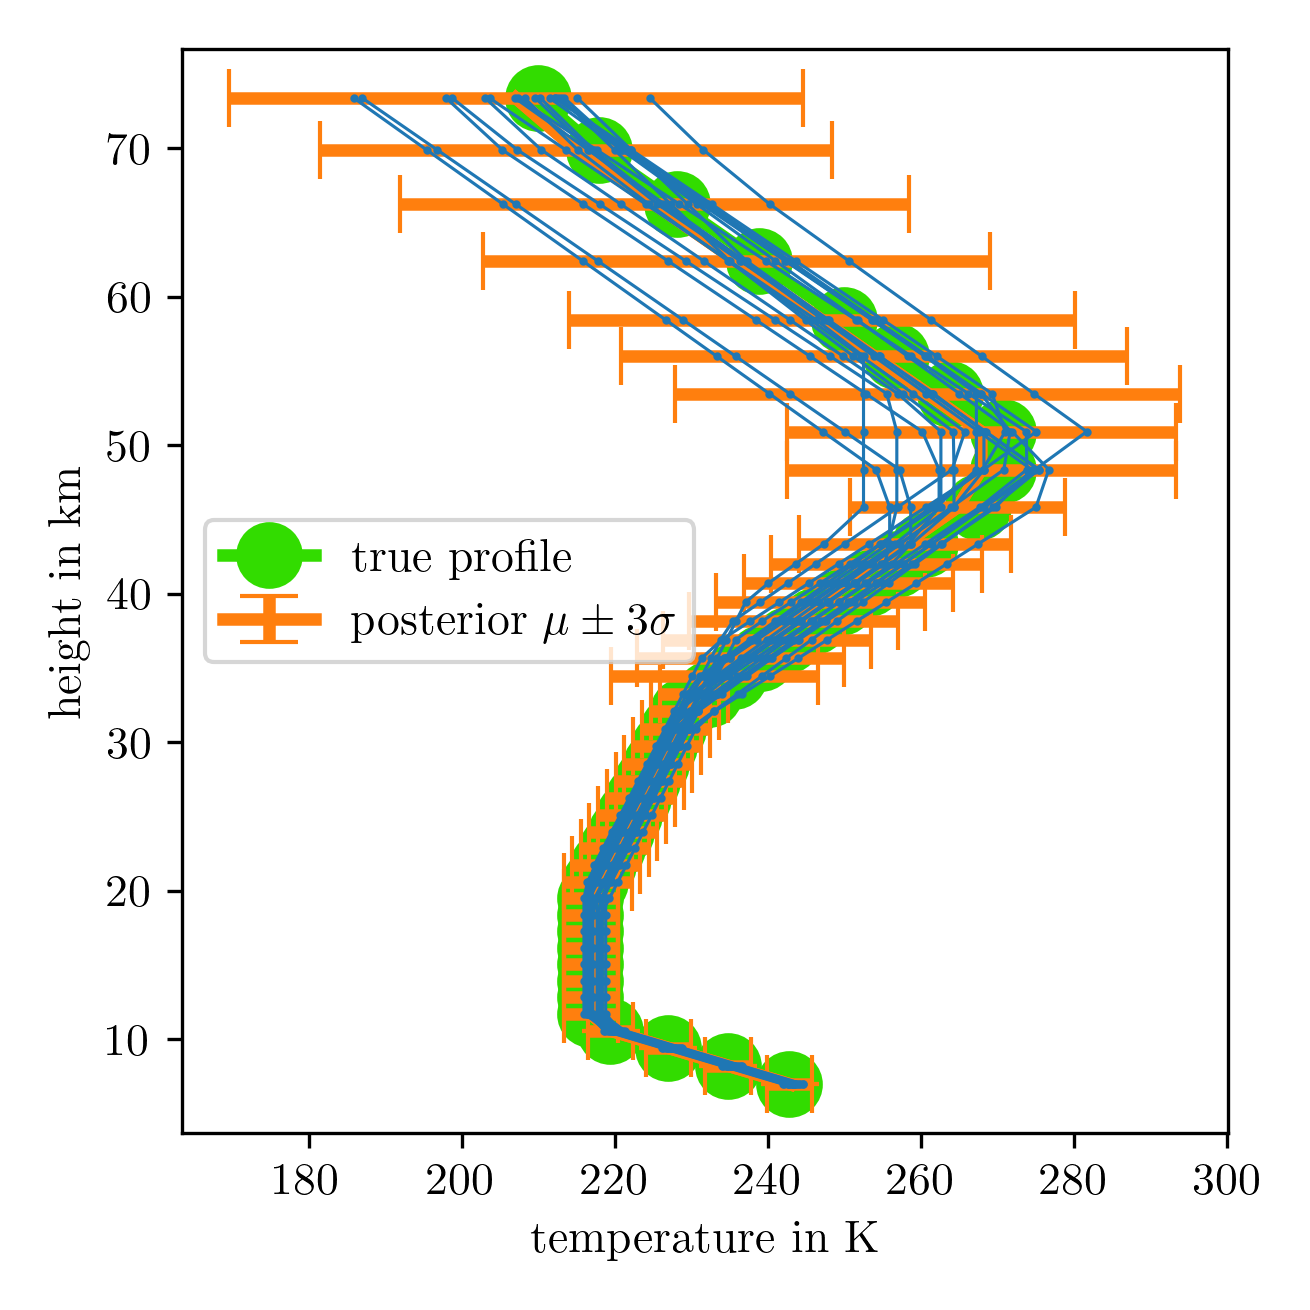
\includegraphics{TempPostMeanSigm.png} 
	\caption[Temperature posterior samples.]{We take samples from the posterior distribution, as plotted in Figures \ref{fig:PostHistTT0} to \ref{fig:PostHistTT3} and plot the corresponding temperature function, see Eq: \ref{eq:tempFunc}. }
	\label{fig:TempPost}
\end{figure}
\cleardoublepage
\begin{figure}[ht!]
	\centering
	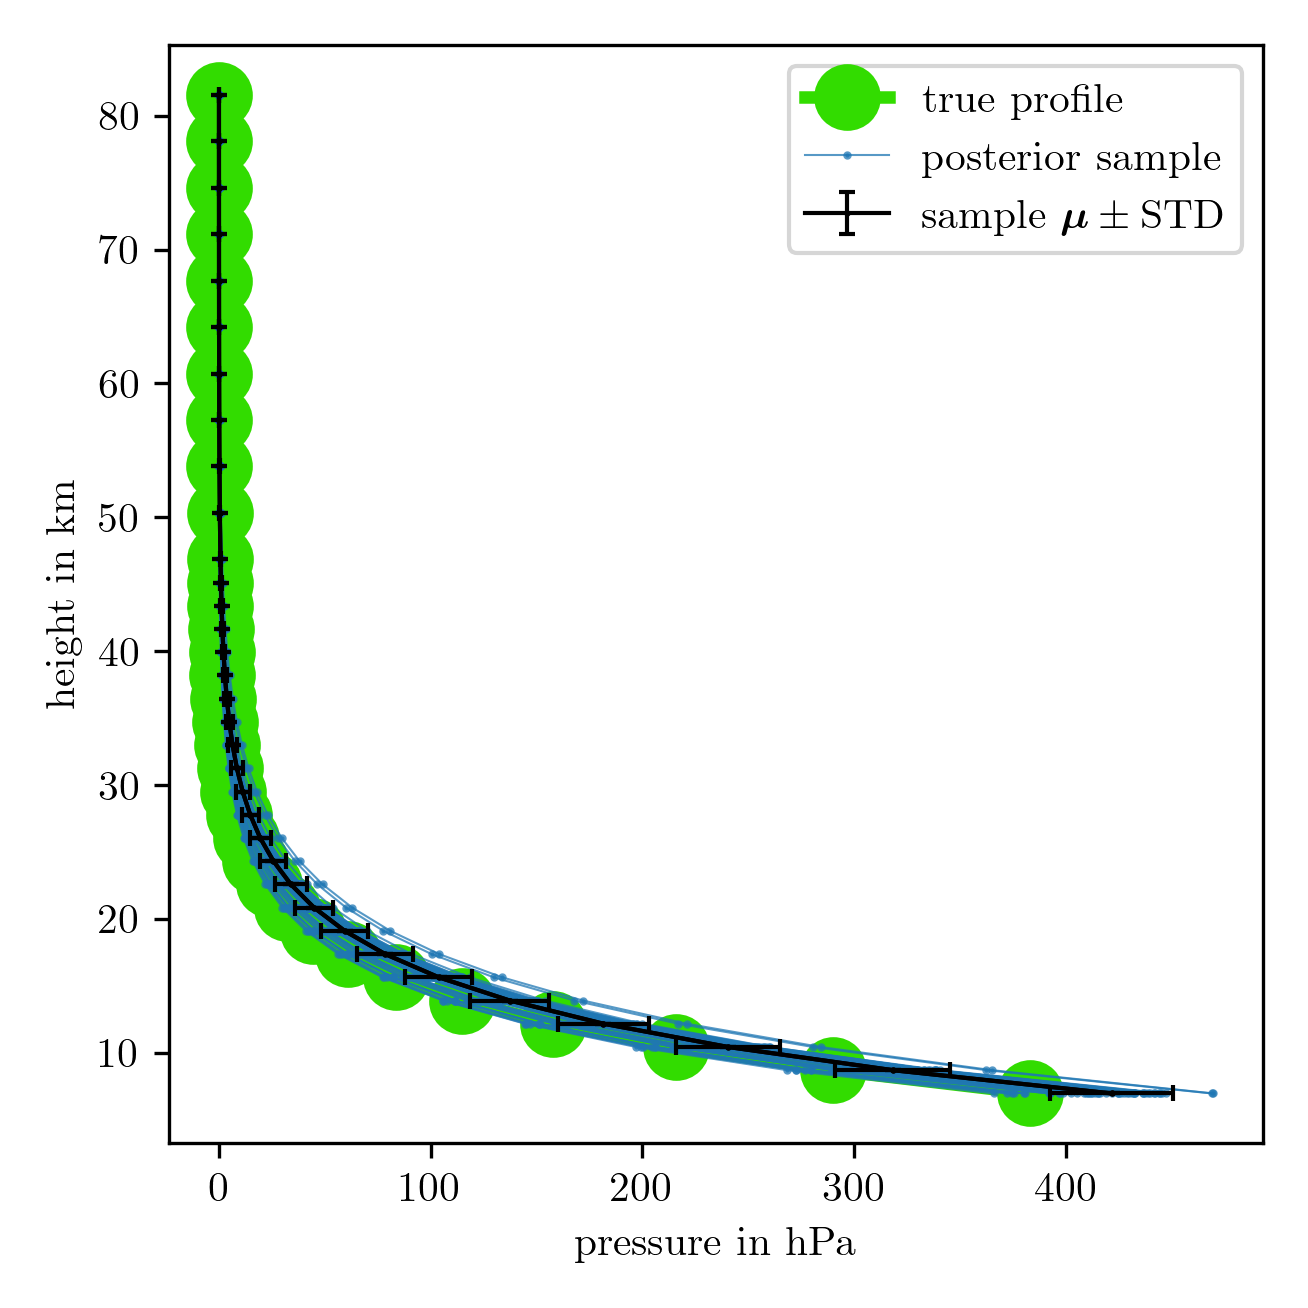
\includegraphics{PressPostMeanSigm.png}
	\caption[Pressure posterior samples.]{We take samples from the posterior distribution, as plotted in Fig. \ref{fig:PostHistTT4} and plot the corresponding pressure function, see Eq: \ref{eq:pressFunc}.}
	\label{fig:PressPost}
\end{figure}

\begin{figure}[ht!]
	\centering
	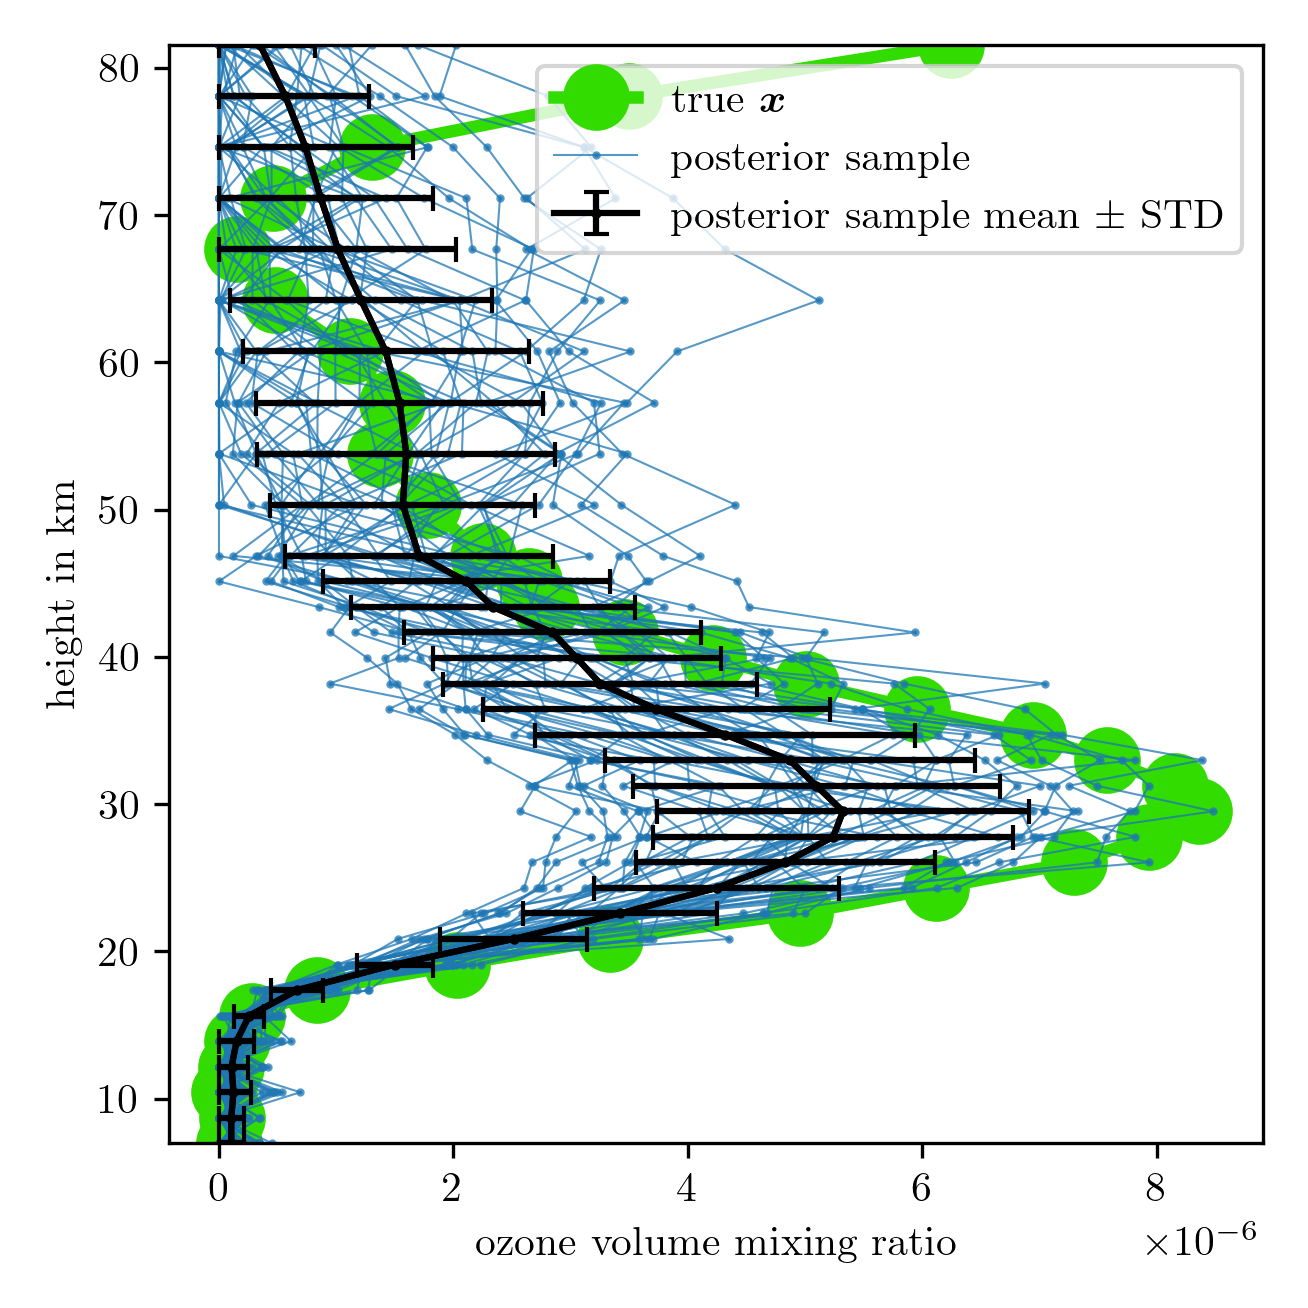
\includegraphics{FullO3Res.png}
	\caption[Pressure posterior samples.]{We take samples from the posterior distribution, as plotted in Fig. \ref{fig:PostHistTT4} and plot the corresponding pressure function, see Eq: \ref{eq:pressFunc}.}
	\label{fig:O3Post}
\end{figure}

\section{Error analysis}
In this section, we estimate errors due to the function approximations of $f(\lambda)$ and $g(\lambda)$ and how these errors propagate to the marginal posterior.
Additionally, we approximate errors of the TT-approximation as well as Monte-Carlo errors when binning up the samples.

\subsubsection{Error due to Approximation of f and g}
\label{sec:fgErros}
When approximating the functions $f(\lambda)$ and $g(\lambda)$, we find that the 3rd-order Taylor series of $f(\lambda)$ and a linear approximation of $g(\lambda)$ in log-space give the smallest error.
The Taylor series truncation error of $f(\lambda)$ is bounded by the fourth order Taylor series $E_f = \underset{\lambda}{\text{arg max}\,} f^{(4)}(\lambda_0)/ 4! \, (\lambda - \lambda_{0} )^4$ and corresponds to an relative error bounded by $20\%$.
Since the maximum absolute error of the approximation $\underset{\lambda}{\text{arg max}\,}|\tilde{g}(\lambda) - g(\lambda) | \approx 1$ corresponds to an relative error of approximately $0.3\%$ and is small compared to $E_f \approx 1e8$ we ignore the approximation error of $g(\lambda)$.
Then the maximum relative propagation error $\underset{\lambda, \gamma}{\text{arg max}\,} 0.5 \gamma  E_f / \log{\pi{(\lambda ,\gamma | \bm{y})}} $ is bound by approximately $5\%$.
\subsubsection{Tensor-train approximation error for the marginal posterior}
We calculate the error of the TT approximation of the marginal posterior with the Wasserstein distance $||x||$.
The wasserstein distance between the normalised true marginal posterior $\pi(\lambda,\gamma|\bm{y})$ and the TT approximation $\tilde{\pi}(\lambda,\gamma|\bm{y})$ is $0.1$.

%When approximating the marginal posterior the maximum relative propagation error $\underset{\lambda , \gamma}{\text{arg max}\,}|\tilde{\pi}(\lambda,\gamma|\bm{y}) - \pi(\lambda,\gamma|\bm{y}) |/ |\pi(\lambda,\gamma|\bm{y})|$ is approximately $100\%$ at $\gamma_{\text{max}}$ and $\lambda_{\text{max}}$, which are the maximum values of the $\lambda$ and $\gamma$ samples and lay in regions with very low probability.
%We consider this error negligible because the absolute error at $\gamma_{\text{max}}$ and $\lambda_{\text{max}}$ is smaller than $10^{-24} \approx 0$.
%Note that one can reduce the maximum errors when approximation $f(\lambda)$ at the mean of $\pi(\lambda,\gamma|\bm{y})$ instead of the modes since $\pi(\lambda | \bm{y})$ is skewed, but we don't see noticeable differences in the conditional posterior $\pi(\bm{x}|\lambda,\gamma,\bm{y})$ when doing so.
%We consider these errors as tolerable.
$\lVert \pi(\bm{x}_{MH}) - \tilde{\pi}(\bm{x}_{MH}) \rVert / \lVert \pi(\bm{x}_{MH}) \rVert$
$\lVert \mathbb{E}\big[ \bm{x} \big]  -  \mathbb{E} \big[ \tilde{\bm{x}} \big] \rVert_{L^2}$
$\lVert \mathbb{E}  \big[\bm{x}\big] -  \mathbb{E} \big[ \bm{x}_{MH}\big]  \rVert_{L^2}$
\subsubsection{Error due to grid size}
When we calculate the mean and covariance matrix of the full conditional $\pi(\bm{x}|\bm{y})$ we have to bin up the samples of the marginal posterior $\pi(\gamma, \delta |\bm{y})$ or use a TT approximation on a predefined grid with a certain number of grid points, we like to give an estimate for this error as well.
In doing we bin up samples and use the height $\tilde{\pi}(\bm{\theta}^{(k)}_d)$ for a bin $k = 1, \dots, \text{N}_b$ to calculate the mean $\tilde{\mu}_d = \sum_{\text{N}_b} \tilde{\pi}(\bm{\theta}^{(k)}_d) $.
We compare to the sample mean $\bm{\mu}_d = \sum_{k=1}^N \bm{\theta}^{(k)}_d/N$ and calculate the relative error $||\bm{\mu}_{\text{samp}} -\bm{\mu}_{\text{distr}} ||/ || \bm{\mu}_{\text{samp}} ||$
where $\bm{\mu}_{\text{samp}} =(\tilde{\mu}_1, \dots , \tilde{\mu}_D) $ and equivalently $\bm{\mu}_{\text{distr}} =(\tilde{\mu}_1, \dots , \tilde{\mu}_D) $.
Here $d$ refers to the $D = 16$ hyper-parameters $\gamma, \lambda, h_1, h_2, h_3, h_4, h_5, h_6, a_0, a_1, a_2, a_3, a_4, T_0, p_0, b$.

The relative error behaves proportionally to $1/N$, see Fig. \ref{fig:MCError} and Eq. \ref{eq:MCerr}, and we consider a relative error less than $0.1\%$ good enough.
This happens roughly at a bin size of 25, which is our TT grid size.
Note that we exclude the error due to $\tau_{\text{int}}$ the IACT and that we choose the grid according to the sampled values so that the sampling region is the same as the region in which we approximate the posterior distributions.
.\begin{figure}[ht!]
	\centering
	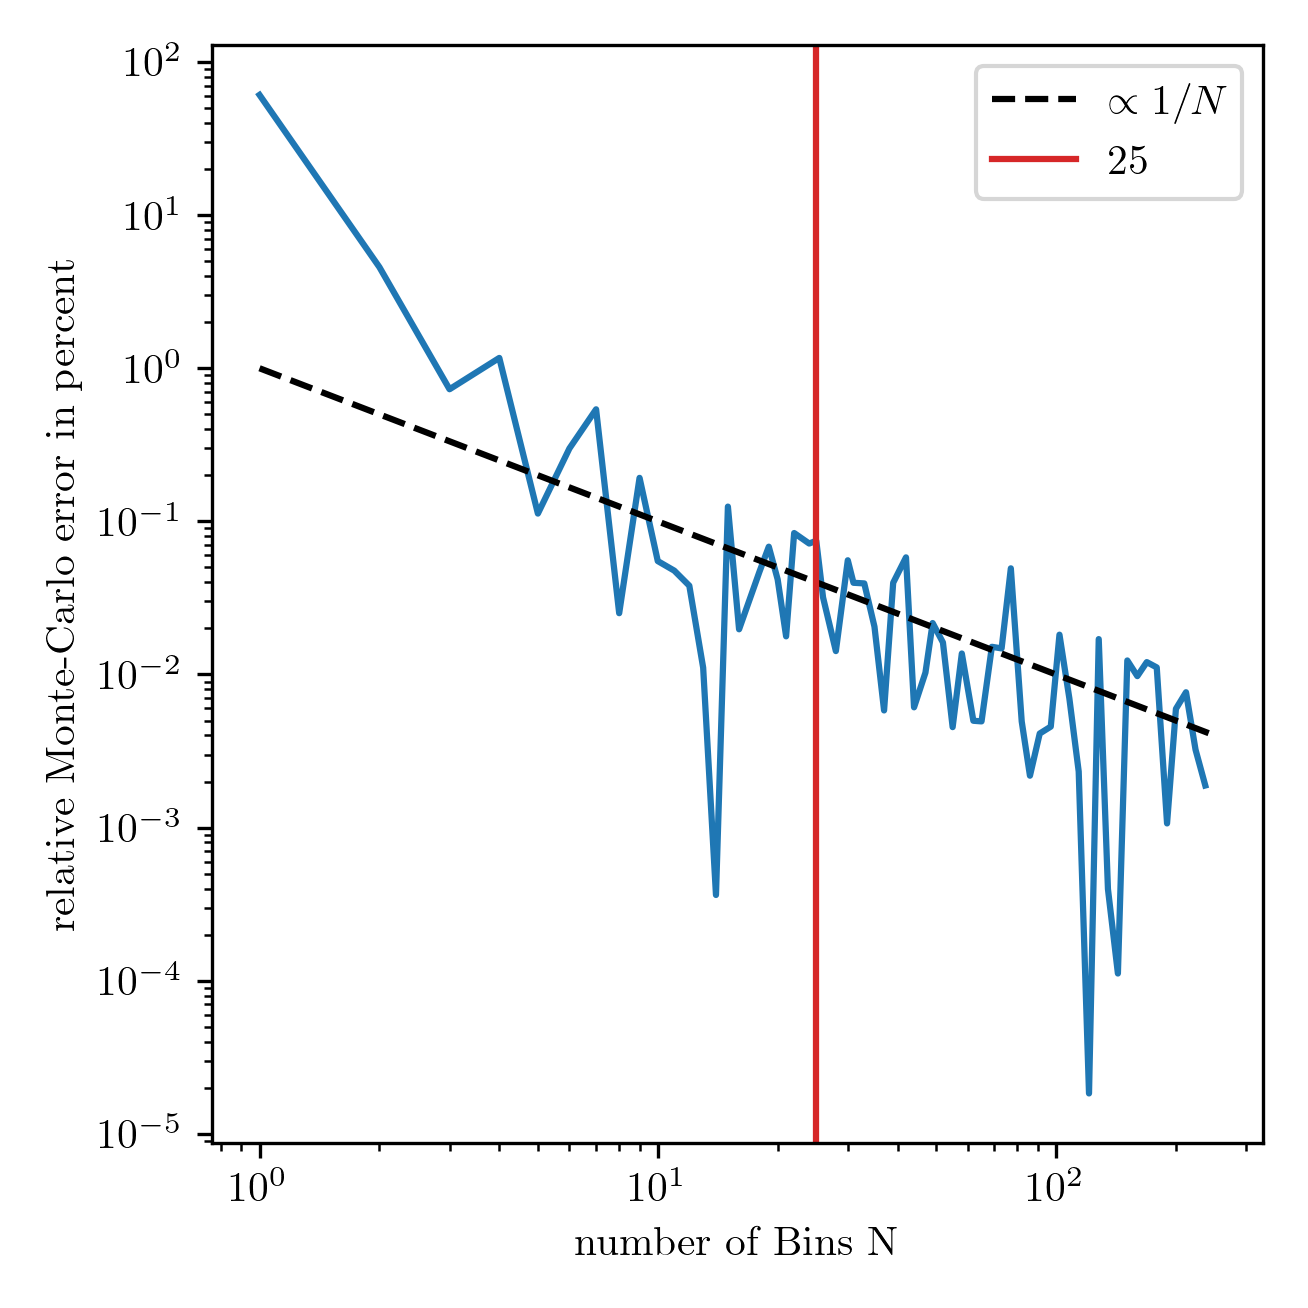
\includegraphics{MeanAssPT.png}
	\caption[Assessment of Monte-Carlo error.]{Assessment of Monte-Carlo error, where we calculate the relative error of the mean due to binning up the samples compared to the sample mean $||\bm{\mu}_{\text{samp}} -\bm{\mu}_{\text{distr}} ||/ || \bm{\mu}_{\text{samp}}||$.}
	\label{fig:MCError}
\end{figure}


%\begin{figure}[thb!]
%	\centering
%	\begin{tikzpicture}
	%		
	%		\node[align=center] at (-1,4) (A)    {$\bm{M A}_L$};
	%		\node[roundnode2] at (-1,2.5) (u)    {$\bm{u}$};
	%		\node[rectnode] at (-1,1) (y)    {$\bm{y}$};
	%		
	%		\node[roundnode2] at (3,6.5) (t)     {$\bm{T}$};
	%		\node[roundnode2] at (-1,6.5) (p)     {$\bm{p}$};
	%		\node[roundnode2] at (1,5) (pt)     {$\bm{p}/\bm{T}$};
	%		\node[roundnode2] at (0,8) (b1)    {$b$};
	%		%\node[roundnode2] at (1,8) (b2)    {$b_2$};
	%		\node[roundnode2] at (-2,8) (h1)    {$h_0$};
	%		\node[roundnode2] at (-1,8) (p0)    {$p_0$};
	%		\node[roundnode2] at (2.25,8) (ht)    {$\bm{h}$};
	%		\node[roundnode2] at (3.25,8) (ct)    {$T_0$};
	%		\node[roundnode2] at (4.25,8) (at)    {$\bm{a}$};
	%		
	%		%Lines
	%		\draw[->, very thick] (u.south) -- (y.north);
	%		\draw[->, mydotted, very thick] (A.south) -- (u.north);
	%		
	%		\draw[->, mydotted, very thick] (p.south east) -- (pt.north west);
	%		\draw[->, mydotted, very thick] (t.south west) -- (pt.north east);
	%		\draw[->, mydotted, very thick] (pt.south west) -- (A.east);
	%		\draw[->, mydotted, very thick] (h1.south) -- (p.north west);
	%		\draw[->, mydotted, very thick] (p0.south) -- (p.north);
	%		\draw[->, mydotted, very thick] (b1.south) -- (p.north east); 
	%		%\draw[->, very thick] (b2.south) -- (p.east); 
	%		
	%		\draw[->, mydotted, very thick] (ht.south) -- (t.north west);
	%		\draw[->, mydotted, very thick] (ct.south) -- (t.north);
	%		\draw[->, mydotted, very thick] (at.south) -- (t.north east);
	%		
	%		\node[align =center] at (-5,8) (T1) {posterior \\ over hyper-parameters \\ $\pi(h_0, p_0, b, \bm{h}, T_0, \bm{a}| \bm{y})$};
	%		
	%		\node[fit=(h1)(at),draw,dotted,black, rounded corners] {};
	%	\end{tikzpicture} 
%	\caption[Directed acyclic Graph for pressure and temperature.]{Conditioned on an ozone profile the posterior of the hyper-parameters describing pressure and temperature is given as in Eq. \ref{eq:}. Since pressure and temperature go into the forward model as $\bm{p}/\bm{T}$ they are highly correlated but the pressure is the dominant parameter, see Fig. 
	%		\ref{fig:PriorPressOverTemp} and \ref{fig:SeaLevelHist}. Note that here we use the updated forward model $\bm{M} \bm{A}_L$ and conditioned on a $\gamma$ sample from the previously evaluated marginal posterior see Fig. \ref{fig:MargPostHistTT}. }
%	\label{fig:DAGPT}
%\end{figure}